% !TEX spellcheck = en_US

%
% Paper latex template
%
%
% Parameters
%

\RequirePackage{etoolbox}
\newtoggle{full}          % false = conference version; true = full version
\newtoggle{showoverflow}  % true  = show overflows
\newtoggle{allowtodo}     % false = remove todo command
\newtoggle{allowexpl}     % false = remove explanations
\newtoggle{anonymous}     % true  = anonymous
\newtoggle{submission}    % true  = submission (force llncs style for crypto)
\newtoggle{llncs}

\providetoggle{forcefull} % true = force full version from outside (see paper-full.tex)
\providetoggle{forceconf} % true = force conf version from outside (see paper-conf.tex)
\iftoggle{forcefull}{\toggletrue{full}}{\iftoggle{forceconf}{\togglefalse{full}}{
    \toggletrue{full}     % default value for full
  }}
 
\toggletrue{full}
%\toggletrue{showoverflow} % default value for showoverflow
\togglefalse{allowtodo}    % default value for allowtodo
\togglefalse{allowexpl}    % default value for allowexpl
\togglefalse{anonymous}    % default value for anonymous

%\togglefalse{allowtodo}
%\togglefalse{allowexpl}

\ifboolexpr{togl{full} and (not togl{submission})}{
  \togglefalse{llncs}
}{
  \toggletrue{llncs}
}

%
% Document class
%
\iftoggle{llncs}{
  \documentclass[envcountsame,runningheads]{llncs}
}{
  \documentclass[11pt,envcountsame,runningheads]{llncs+}
  \ifboolexpr{not (togl{allowtodo})}{
   %\usepackage[a4paper, hmargin=2cm, vmargin=2cm, marginparwidth=1.8cm]{geometry}
   \usepackage[a4paper]{geometry}
  }{
    %\usepackage[a4paper, left=0.8cm, right=3.2cm, vmargin=2cm, marginparwidth=2.8cm]{geometry}
    \usepackage[a4paper]{geometry}
  }
}
\pagestyle{plain}
\makeatletter
%\def\tableofcontents{\def\authcount##1{\setcounter{auco}{##1}\setcounter{@auth}{1}}\@starttoc{toc}}
\makeatother

%
% Custom header
%

% !TeX root = ../main.tex
% !TEX root = ../main.tex
% !TEX spellcheck = en-US

%
% Packages
%

% Standard packages
\usepackage[utf8]{inputenc}
\usepackage[T1]{fontenc}
\usepackage{amsmath}
\usepackage{amssymb}
\usepackage{mathtools}
\usepackage{booktabs}
\usepackage{array}
\usepackage{tabu}
\usepackage{cite}
\usepackage{url}
\usepackage{xcolor}
\usepackage{xspace}
\usepackage{xargs}
\usepackage{multirow,bigdelim} %bigdelim added by julia, supplements multirow by supporting brackets over multiple rows
\usepackage{hhline} % for YGC comparison table
\usepackage{verbatimbox} % for crypto games
\usepackage{multirow} % for crypto games
\usepackage{scalerel} % for crypto games
\usepackage{tikz} % for FAKE circuit description
\usetikzlibrary{circuits.logic.US} % for FAKE circuit description
\newtheorem{observation}{Observation}
\usepackage{adjustbox} % for table column header rotation
\usepackage{array} % for table column header rotation

\setcounter{secnumdepth}{3} % to make subsubsections have numbers

\usepackage[textsize=small]{todonotes}
\iftoggle{allowtodo}{
  % add xspace to todo command (http://tex.stackexchange.com/a/68741)
  \makeatletter
  \expandafter\apptocmd\csname\string\todo\endcsname{\xspace}{}{}
  \makeatother
  
  \newcommandx{\pad}[2][1=]{\todo[linecolor=cyan, backgroundcolor=cyan!25, bordercolor=cyan,#1]{Pierre-Alain: #2}}
  \newcommandx{\julia}[2][1=]{\todo[linecolor=blue, backgroundcolor=blue!25, bordercolor=blue,#1]{Julia: #2}}
  \newcommandx{\david}[2][1=]{\todo[linecolor=red, backgroundcolor=red!25, bordercolor=red,#1]{David: #2}}
  \newcommandx{\sophia}[2][1=]{\todo[linecolor=green, backgroundcolor=green!25, bordercolor=green,#1]{Sophia: #2}}
  \newcommandx{\leo}[2][1=]{\todo[linecolor=yellow, backgroundcolor=yellow!25, bordercolor=yellow,#1]{Leo: #2}}  
}
{
  \newcommandx{\pad}[2][1=]{}
  \newcommandx{\julia}[2][1=]{}
  \newcommandx{\david}[2][1=]{}
  \newcommandx{\sophia}[2][1=]{}
  \newcommandx{\leo}[2][1=]{} 
}

\iftoggle{allowexpl}{
  \newcommand{\expl}[1]{\todo[inline,linecolor=red, backgroundcolor=orange!25, bordercolor=red]{Comment: #1}}
}
{
 \newcommand{\expl}[1]{}
}

% Personal packages
\usepackage{games}

% Hyperref
\usepackage[pdfpagelabels=true]{hyperref}
\hypersetup{
%  linktoc = page,
  pdfpagemode = UseNone,
  colorlinks,
  linkcolor={red!50!black},
  citecolor={blue!50!black},
  urlcolor={blue!80!black}
}

%\iftoggle{full}{
%  \renewcommand*{\backref}[1]{}
%  \renewcommand*{\backrefalt}[4]{
%    \ifcase #1
%    (Not cited.)
%    \or
%    (Page~#2.)
%    \else
%    (Pages~#2.)
%    \fi
%  }
%  \renewcommand*{\backrefsep}{, }
%  \renewcommand*{\backreftwosep}{ and~}
%  \renewcommand*{\backreflastsep}{, and~}
%}{}

\makeatletter
\AtBeginDocument{
  \hypersetup{
    pdftitle = {\@title},
    pdfauthor = {\@author}
  }
}
\makeatother

% cleveref
\usepackage[capitalize]{cleveref}

% Nice headings
\newcommand{\heading}[1]{{\vspace{6pt}\noindent\sc{#1.}}}
% \newcommand{\heading}[1]{\paragraph{\sc #1.}}
%
% Misc
% %

\iftoggle{showoverflow}{
  \overfullrule=10pt
}{}
\newcommand{\alert}[1]{\textcolor{red}{#1}}
%
% Figures & Captions
%

\newcommand*{\repeatcaption}[2]{
  \renewcommand{\thefigure}{\ref{#1}}
  \caption{#2 (reminder)}
}

%
% References
%

\iftoggle{full}{
  \newcommand*{\appref}[1]{Appendix~\ref{#1}}
}{
  \newcommand*{\appref}[1]{the full version of this paper~\cite{cryptoeprint:2017:1111}}
}

\newcommand{\passstring}{pass-string}
\newcommand{\Passstring}{Pass-string}

%
% Games
%
\newcounter{game}
\def\newGames{\setcounter{game}{0}}
\def\newGame#1{\xdef\prevGame{\arabic{game}}\addtocounter{game}{1}%
  \expandafter\xdef\csname game#1\endcsname{\arabic{game}}}
\def\thisGame{\arabic{game}}
\def\refGame#1{\csname game#1\endcsname}
\renewcommand{\Game}[1][]{\if!#1!\textrm{Game}\xspace\else\textrm{Game \ensuremath{#1}}\fi}
\newcommand{\Games}[1][]{\if!#1!\textrm{Games}\xspace\else\textrm{Games \ensuremath{#1}}\fi}
% usage: 
% \newGame{name} -- inits new Game called name
% \refGame{name} -- Number of Game called name
% \thisGame -- Number of current Game
% \prevGame -- Number of previous Game


%
% General and Math commands
%

% Abbreviations
\newcommand{\etal}{\emph{et al.}\xspace}

% Math sets and groups
\newcommand{\Z}{\mathbb{Z}}
\newcommand{\F}{\mathbb{F}}
\newcommand{\N}{\mathbb{N}}
\newcommand{\G}{\mathbb{G}}

% Math misc
\makeatletter
\newcommand\suchthat{%
 \@ifstar
  {\mathrel{}\middle|\mathrel{}}
  {\mid}%
}
\makeatother

\newcommand{\cind}{\ensuremath{\stackrel{c}{\approx}\xspace}}
\newcommand{\defeq}{\coloneqq}
\newcommand{\eqdef}{\eqqcolon}
\newcommand{\eeq}{\overset{{}_{?}}{=}}

%tikz stuff
\usepackage{tikz}
\usetikzlibrary{shapes.misc,shapes}
\usetikzlibrary{positioning}
\usetikzlibrary{calc}
\usetikzlibrary{arrows}
\usetikzlibrary{decorations.markings}
\def\shortbib{1}

%
% General Crypto commands
%

% Algorithms
\newcommand{\getsr}{\stackrel{{}_\$}{\leftarrow}}

% Experiments / Game
\newcommand{\Ax}{\mathcal{A}}
\newcommand{\Bx}{\mathcal{B}}
\newcommand{\Dx}{\mathcal{D}}
\newcommand{\Ex}{\mathcal{E}}
\newcommand{\Fx}{\mathcal{F}}
\newcommand{\Sx}{\mathcal{S}}
\newcommand{\Ux}{\mathcal{U}}
\newcommand{\pw}{\mathsf{pw}}
\newcommand{\sid}{\mathsf{sid}}
%\newcommand{\key}{\mathsf{key}}
\newcommand{\state}{\mathsf{state}}
\newcommand{\accept}{\mathsf{accept}}
\newcommand{\reject}{\mathsf{reject}}
\newcommand{\terminate}{\mathsf{terminate}}

\newcommand{\Exp}{\mathsf{Exp}}

\newcommand{\secu}{\web{sec}}
\newcommand{\SECU}{\web{SEC}}

\newsavebox{\fboxenvbox}
\newenvironment{fboxenv}
    {\begin{lrbox}{\fboxenvbox}}
    {\end{lrbox}\fbox{\usebox{\fboxenvbox}}}
    
% Protocol flows
\newcommand*{\Rflow}[2][10em]{\ensuremath{\xrightarrow{\smash{\makebox[#1][c]{$#2$}}}}}
\newcommand*{\Lflow}[2][10em]{\ensuremath{\xleftarrow{\smash{\makebox[#1][c]{$#2$}}}}}
\newcommand*{\LRflow}[3][10em]{\ensuremath{\xleftrightarrow[\smash{\makebox{$#2$}}]{\smash{\makebox[#1][c]{$#3$}}}}}
\newcommand*{\LRsbflow}[3][10em]{\ensuremath{\xleftrightharpoons[\smash{\makebox{$#2$}}]{\smash{\makebox[#1][c]{$#3$}}}}}
\newcommand*{\LRsflow}[3][4em]{\ensuremath{\xleftrightharpoons[\smash{\makebox{$#2$}}]{\smash{\makebox[#1][c]{$#3$}}}}}
\newcommand*{\Rsflow}[2][4em]{\ensuremath{\xrightarrow{\smash{\makebox[#1][c]{$#2$}}}}}
\newcommand*{\Rsmallflow}[2][2em]{\ensuremath{\xrightarrow{\smash{\makebox[#1][c]{$#2$}}}}}
\newcommand*{\Lsflow}[2][4em]{\ensuremath{\xleftarrow{\smash{\makebox[#1][c]{$#2$}}}}}

% Crypto misc

\newcommand{\eps}{\varepsilon}
\DeclareMathOperator{\negl}{\mathsf{negl}}

% Hard problems (uppercase) and associated experiment names (lowercase)
\newcommand{\hardprobfont}[1]{\texorpdfstring{\ensuremath{\textsf{#1}}}{#1}}
\newcommand{\DL}{\hardprobfont{DL}\xspace}
\newcommand{\dl}{\hardprobfont{dl}\xspace}
\newcommand{\DHtup}{\hardprobfont{DH}\xspace}    % DH tuple
\newcommand{\DDH}{\hardprobfont{DDH}\xspace}
\newcommand{\ddh}{\hardprobfont{ddh}\xspace}
\newcommand{\MDDH}{\hardprobfont{MDDH}\xspace}
\newcommand{\mddh}{\hardprobfont{mddh}\xspace}
\newcommand{\DLin}{\hardprobfont{DLin}\xspace}
\newcommand{\dlin}{\hardprobfont{dlin}\xspace}
\newcommand{\XDH}{\hardprobfont{XDH}\xspace}
\newcommand{\xdh}{\hardprobfont{xdh}\xspace}
\newcommand{\CDH}{\hardprobfont{CDH}\xspace}
\newcommand{\cdh}{\hardprobfont{cdh}\xspace}
\newcommand{\SXDH}{\hardprobfont{SXDH}\xspace}
\newcommand{\sxdh}{\hardprobfont{sxdh}\xspace}
\newcommand{\BDDH}{\hardprobfont{BDDH}\xspace}
\newcommand{\bddh}{\hardprobfont{bddh}\xspace}
\newcommand{\BDDHI}{\hardprobfont{BDDHI}\xspace}
\newcommand{\bddhi}{\hardprobfont{bddhi}\xspace}
\newcommand{\klin}{\texorpdfstring{\kappa}{k}}
\newcommand*{\Lin}[1]{\texorpdfstring{\ensuremath{{#1\text{-}\textsf{Lin}}}}{#1-Lin}\xspace}
\newcommand*{\lin}[1]{\texorpdfstring{\ensuremath{{#1\text{-}\textsf{lin}}}}{#1-lin}\xspace}
\newcommand{\coll}{\hardprobfont{coll}\xspace}

%
% Commands specific to the paper 
%

\newcommand{\web}[1]{\texttt{#1}}

% bits
\newcommand{\bits}{\{0,1\}}
\newcommand{\bitsn}{\{0,1\}^{n}}

% Notions
\newcommand{\notionfont}[1]{\texorpdfstring{\ensuremath{\textsf{#1}}}{#1}}
\newcommand{\WRSS}{\notionfont{WRSS}\xspace}
\newcommand{\RSS}{\notionfont{RSS}\xspace}
\newcommand{\UC}{\textsf{UC}\xspace}
\newcommand{\AKE}{\textsf{AKE}\xspace}
\newcommand{\PAKE}{\textsf{PAKE}\xspace}
\newcommand{\iPAKE}{\textsf{iPAKE}\xspace}
\newcommand{\liPAKE}{\ensuremath{\ell}\textsf{-iPAKE}\xspace}
\newcommand{\FAKE}{\textsf{fPAKE}\xspace}
\newcommand{\FFAKE}{\Fx_\FAKE\xspace}
\newcommand{\FiPAKE}{\Fx_\iPAKE\xspace}
\newcommand{\FliPAKE}{\ensuremath{\Fx_{\ell\notionfont{-iPAKE}}\xspace}}
\newcommand{\Lpw}{\ensuremath{\Lambda_{\mathcal{P}}}}
\newcommand{\Ll}{\ensuremath{\Lambda_{\mathcal{L}}}}
\newcommand{\FpwKE}{\Fx_\notionfont{pwKE}\xspace}
\newcommand{\Fcrs}{\ensuremath{\Fx_\notionfont{CRS}}\xspace}
\newcommand{\Fic}{\ensuremath{\Fx_\notionfont{IC}}\xspace}
\newcommand{\Fro}{\ensuremath{\Fx_\notionfont{RO}}\xspace}
\newcommand{\Fot}{\ensuremath{\Fx_\notionfont{OT}}\xspace}
\newcommand{\Fsot}{\ensuremath{s\Fx_\notionfont{OT}}\xspace}
\newcommand{\Frfe}{\ensuremath{\Fx_\notionfont{RFE}}\xspace}
\newcommand{\Fsrfe}{\ensuremath{s\Fx_\notionfont{RFE}}\xspace}
\newcommand{\Prfe}{\ensuremath{\Pi_\notionfont{RFE}}\xspace}
\newcommand{\PfakeYGC}{\ensuremath{\FAKE_\notionfont{YGC}}\xspace}
\newcommand{\PfakeRSS}{\ensuremath{\FAKE_\RSS}\xspace}

\newcommand{\ind}{{\mathsf{ind}}}

\newcommand{\INDCPA}{\texttt{IND-CPA}\xspace}
\newcommand{\indcpa}{\mathsf{ind-cpa}}
\newcommand{\INDCCA}{\texttt{IND-CCA}\xspace}
\newcommand{\indcca}{\mathsf{ind-cca}}
\newcommand{\CPA}{\texttt{CPA}\xspace}
\newcommand{\CCA}{\texttt{CCA}\xspace}
\newcommand{\IND}{\texttt{IND}\xspace}
\newcommand{\INTCTXT}{\texttt{INT-CTXT}\xspace}
\newcommand{\intctxt}{\mathsf{int-ctxt}\xspace}
\newcommand{\authenc}{\mathsf{authenc}\xspace}

% Signature scheme
\newcommand{\SigGen}{\mathsf{SigGen}\xspace}
\newcommand{\Sign}{\mathsf{Sign}\xspace}
\newcommand{\Vfy}{\mathsf{Vfy}\xspace}

% Secret sharing
\newcommand{\Share}{\ensuremath{\mathsf{Share}}\xspace}
\newcommand{\Reconstruct}{\ensuremath{\mathsf{Reconstruct}}\xspace}
\newcommand{\tc}{\ensuremath{\tilde{c}}}
\newcommand{\bA}{\ensuremath{\bar{A}}}


% SPHF
\newcommand{\HashKG}{\ensuremath{\mathsf{HashKG}}\xspace}
\newcommand{\ProjKG}{\ensuremath{\mathsf{ProjKG}}\xspace}
\newcommand{\Hash}{\ensuremath{\mathsf{Hash}}\xspace}
\newcommand{\ProjHash}{\ensuremath{\mathsf{ProjHash}}\xspace}

\newcommand{\hk}{\mathsf{hk}}
\newcommand{\hp}{\mathsf{hp}}

% Security / games
\newcommand{\Env}{\ensuremath{\mathcal{Z}}\xspace}
\newcommand{\AdvA}{\ensuremath{\mathcal{A}}\xspace}
\newcommand{\AdvB}{\ensuremath{\mathcal{B}}\xspace}
\newcommand{\BCDH}{\ensuremath{\AdvB_{\CDH}}\xspace}
\newcommand{\Sim}{\ensuremath{\mathcal{S}}\xspace}
\newcommand{\Func}{\ensuremath{\mathcal{F}}\xspace}

\newcommand{\Adv}{\mathsf{Adv}}
\newcommand{\Succ}{\mathsf{Succ}}

\newcommand*{\procfont}[1]{\ensuremath{\textbf{#1}}}
\newcommand{\Initialize}{{\procfont{Initialize}}}
\newcommand{\Finalize}{{\procfont{Finalize}}}

\newcommand{\real}{\mathtt{real}}
\newcommand{\ideal}{\mathtt{ideal}}
\newcommand{\Init}{\texttt{Init}\xspace}

% CRS, ...
\newcommand{\param}{\mathsf{param}}
\newcommand{\crs}{\mathsf{crs}}

% UC
\newcommand{\NewSession}{\web{NewSession}\xspace}
\newcommand{\TestPwd}{\web{TestPwd}\xspace}
\newcommand{\NewKey}{\web{NewKey}\xspace}
\newcommand{\ListIC}{\ensuremath{\Lambda_{IC}}\xspace}
\newcommand{\ListRO}{\ensuremath{\Lambda_{RO}}\xspace}
\newcommand{\ListCDH}{\ensuremath{\Lambda_{CDH}}\xspace}
\newcommand{\ListOT}{\ensuremath{\Lambda_{OT}}\xspace}
\newcommand{\role}{\web{role}\xspace}
\newcommand{\rolereceiver}{\web{receiver}\xspace}
\newcommand{\rolesender}{\web{sender}\xspace}
\newcommand{\leakage}{\ensuremath{L}}
\newcommand{\leakageclose}{\ensuremath{\leakage_{c}}}
\newcommand{\leakagefar}{\ensuremath{\leakage_{f}}}
\newcommand{\leakagemiddle}{\ensuremath{\leakage_{m}}}

% BPR model
\newcommand{\nbusers}{{n_u}}
\newcommand{\Reveal}{\texttt{Reveal}\xspace}
\newcommand{\Execute}{\texttt{Execute}\xspace}
\newcommand{\Send}{\texttt{Send}\xspace}
\newcommand{\Receive}{\texttt{Receive}\xspace}
\newcommand{\Corrupt}{\texttt{Corrupt}\xspace}
\newcommand{\Test}{\texttt{Test}\xspace}

\newcommand{\fresh}{\mathsf{fresh}\xspace}
\newcommand{\fsfresh}{\mathsf{fs\text{-}fresh}\xspace}
\newcommand{\Win}{\mathsf{Win}\xspace}
\newcommand{\Coll}{\mathsf{Coll}\xspace}

\newcommand{\true}{\texttt{True}\xspace}
\newcommand{\false}{\texttt{False}\xspace}

\newcommand{\Extract}{\mathsf{Extract}\xspace}
\newcommand{\Start}{\texttt{Start}\xspace}

\newcommand{\Encode}{\mathsf{Encode}\xspace}
\newcommand{\Decode}{\mathsf{Decode}\xspace}
\newcommand{\Encrypt}{\mathcal{E}\xspace}
\newcommand{\Decrypt}{\mathcal{D}\xspace}

%Local paper
\newcommand{\msk}[2]{\ensuremath{m(#1, #2)}}


% table formatting:
\newcolumntype{L}[1]{>{\raggedright\let\newline\\\arraybackslash\hspace{0pt}}m{#1}}
\newcolumntype{C}[1]{>{\centering\let\newline\\\arraybackslash\hspace{0pt}}m{#1}}
\newcolumntype{R}[1]{>{\raggedleft\let\newline\\\arraybackslash\hspace{0pt}}m{#1}}

% MISC:
\newcommand{\xor}{\ensuremath{\oplus}}
\newcommand{\yes}{\ensuremath{\checkmark}}
\newcommand{\no}{}
\newcommand{\booland}{\ensuremath{\wedge}}
\newcommand{\boolor}{\ensuremath{\vee}}
\newcommand{\algfont}[1]{\ensuremath{\mathsf{#1}}}
%\newcommand{\negl}{\ensuremath{negl}}    % already present in main FAKE macros file
\newcommand{\for}{\ensuremath{\mbox{ for }}}
\newcommand{\secarg}[1]{{\color{red} #1}}

% parties:
\newcommand{\client}{\ensuremath{\mathcal{C}}}
\newcommand{\server}{\ensuremath{\mathcal{S}}}
\newcommand{\Party}{\ensuremath{\mathcal{P}}}
\newcommand{\SimYGCRFE}{\ensuremath{\Sim_{\notionfont{RFE}}}}
\newcommand{\SimYGCFAKE}{\ensuremath{\Sim_{\FAKE}}}
\newcommand{\sender}{\ensuremath{\mathcal{S}}}
\newcommand{\receiver}{\ensuremath{\mathcal{R}}}
\newcommand{\oracle}{\ensuremath{\mathcal{O}}}

% 0/1 party terminology:
\newcommand{\firstindex}{\ensuremath{0}}
\newcommand{\secondindex}{\ensuremath{1}}
\newcommand{\firstparty}{\ensuremath{\Party_{\firstindex}}}
\newcommand{\secondparty}{\ensuremath{\Party_{\secondindex}}}
\newcommand{\firstpw}{\ensuremath{\pw_{\firstindex}}}
\newcommand{\secondpw}{\ensuremath{\pw_{\secondindex}}}
\newcommand{\firstkey}{\ensuremath{\key_{\firstindex}}}
\newcommand{\secondkey}{\ensuremath{\key_{\secondindex}}}

\newcommand{\aindex}{\ensuremath{i}}
\newcommand{\otherindex}{\ensuremath{1-\aindex}}
\newcommand{\aparty}{\ensuremath{\Party_{\aindex}}}
\newcommand{\otherparty}{\ensuremath{\Party_{\otherindex}}}
\newcommand{\apw}{\ensuremath{\pw_{\aindex}}}
\newcommand{\otherpw}{\ensuremath{\pw_{\otherindex}}}
\newcommand{\akey}{\ensuremath{\key_{\aindex}}}
\newcommand{\otherkey}{\ensuremath{\key_{\otherindex}}}

% digital objects:
\newcommand{\bit}{\ensuremath{\mathsf{b}}}
%\newcommand{\pw}{\ensuremath{\mathsf{pw}}}    % already present in main FAKE macros file
\newcommand{\pwclient}{\ensuremath{\pw^{\client}}}
\newcommand{\pwserver}{\ensuremath{\pw^{\server}}}
\newcommand{\secretshare}{\ensuremath{\mathsf{s}}}
\newcommand{\random}{\ensuremath{\mathsf{r}}}
\newcommand{\randomclient}{\ensuremath{\random^{\client}}}
\newcommand{\randomserver}{\ensuremath{\random^{\server}}}
\newcommand{\transcript}{\ensuremath{\tau}}
\newcommand{\hdist}{\ensuremath{d}}

% encryption:
\newcommand{\msg}{\ensuremath{\mathsf{msg}}}
\newcommand{\ctext}{\ensuremath{\mathsf{ctext}}}
\newcommand{\keygen}{\ensuremath{\mathsf{KeyGen}}}
\newcommand{\enc}{\ensuremath{\mathsf{Enc}}}
\newcommand{\dec}{\ensuremath{\mathsf{Dec}}}
\newcommand{\key}{\ensuremath{\mathsf{k}}}
\newcommand{\sk}{\ensuremath{\mathsf{sk}}}
\newcommand{\pk}{\ensuremath{\mathsf{pk}}}
\newcommand{\vk}{\ensuremath{\mathsf{vk}}}

% sizes:
\newcommand{\pwlen}{\ensuremath{n}} 
\newcommand{\alphabetsize}{\ensuremath{p}} 
\newcommand{\rank}{\ensuremath{k}} %rank of RSS/ECC, mostly k in the literature but this clashes with our key notation
% \newcommand{\keylen}{\ensuremath{n}} %not used so far
% \newcommand{\threshold}{\ensuremath{t}} %not used so far
\newcommand{\secparam}{\ensuremath{\lambda}}
\newcommand{\SEC}{\secparam}

% security terms:
\newcommand{\simulator}{\ensuremath{\mathcal{S}}}
\newcommand{\advantage}{\ensuremath{\mathsf{Adv}}}
\newcommand{\adversary}{\ensuremath{\mathcal{A}}}
\newcommand{\challenger}{\ensuremath{\mathcal{C}}}
%\newcommand{\game}{\ensuremath{\mathsf{Game}}}
\newcommand{\priv}{\ensuremath{\mathsf{priv}}}
\newcommand{\obliv}{\ensuremath{\mathsf{obliv}}}
\newcommand{\oblivnotpriv}[1]{\framebox{#1}}
\newcommand{\privnotobliv}[1]{\colorbox{gray}{#1}}

% #1: secparam, #2: adversary, #3: gbscheme, #4: simulator:
\newcommand{\oblivgame}[4]{\ensuremath{\mathsf{OblivSim}^{#2}_{#3, #4}(1^{#1})}} 
\newcommand{\privgame}[4]{\ensuremath{\mathsf{PrivSim}^{#2}_{#3, #4}(1^{#1})}} 
\newcommand{\authgame}[3]{\ensuremath{\mathsf{Aut}^{#2}_{#3}(1^{#1})}}
\newcommand{\garbledoutputrandomnessgame}[3]{\ensuremath{\mathsf{GOutRand}^{#2}_{#3}(1^{#1})}}
\newcommand{\inputindependencegame}[5]{\ensuremath{\mathsf{InpInd}^{#2}_{#3, #4, #5}(1^{#1})}}
\newcommand{\strongobliviousnessgame}[6]{\ensuremath{\mathsf{SOblivSim}^{#2}_{#3, #4, #5, #6}(1^{#1})}}
\newcommand{\stronggarbledoutputrandomnessgame}[5]{\ensuremath{\mathsf{SGOutRand}^{#2}_{#3, #4, #5}(1^{#1})}}

\newcommand{\oblivadv}[4]{\ensuremath{\mathsf{OblivAdv}_{#3, #4}(1^{#1}, #2)}}
\newcommand{\privadv}[4]{\ensuremath{\mathsf{PrivAdv}_{#3, #4}(1^{#1}, #2)}}
\newcommand{\garbledoutputrandomnessadv}[3]{\ensuremath{\mathsf{GOutRandAdv}_{#3}(1^{#1}, #2)}}
\newcommand{\inputindependenceadv}[5]{\ensuremath{\mathsf{InpIndAdv}_{#3, #4, #5}(1^{#1}, #2)}}
\newcommand{\strongobliviousnessadv}[6]{\ensuremath{\mathsf{SOblivSimAdv}_{#3, #4, #5, #6}(1^{#1}, #2)}}
\newcommand{\stronggarbledoutputrandomnessadv}[5]{\ensuremath{\mathsf{SGOutRandAdv}_{#3, #4, #5}(1^{#1}, #2)}}

% garbled circuit components
% toy generator / evaluator example:
\newcommand{\generatorname}{Ginny\xspace}
\newcommand{\generatorsymb}{\ensuremath{\mathsf{G}}}
\newcommand{\generatorbit}{\ensuremath{g}}
\newcommand{\evaluatorname}{Evan\xspace}
\newcommand{\evaluatorsymb}{\ensuremath{\mathsf{E}}}
\newcommand{\evaluatorbit}{\ensuremath{e}}
% FUNCTION:
\newcommand{\numinputs}{\ensuremath{n}}
\newcommand{\numoutputs}{\ensuremath{m}}
\newcommand{\numwires}{\ensuremath{q}}
\newcommand{\numgates}{\ensuremath{p}}
\newcommand{\inindices}{\ensuremath{\mathsf{inindices}}}
\newcommand{\gateindices}{\ensuremath{\mathsf{gindices}}}
\newcommand{\outindices}{\ensuremath{\mathsf{outindices}}}
% WIRES:
\newcommand{\wire}{\ensuremath{w}}
\newcommand{\wirelabel}{\ensuremath{W}}
\newcommand{\wireval}{\ensuremath{v}}
\newcommand{\wireperm}{\ensuremath{p}}
\newcommand{\wireinlabelsum}{\ensuremath{M}}
% GATES:
\newcommand{\gate}{\ensuremath{g}}
\newcommand{\ggate}{\ensuremath{G}}
\newcommand{\gates}{\ensuremath{\mathsf{gates}}}
\newcommand{\outindex}{\ensuremath{\mathsf{outindex}}}
\newcommand{\gateinindices}[1]{\ensuremath{\inindices_{#1}}}
\newcommand{\gateoutindex}[1]{\ensuremath{\outindex_{#1}}}
% OTHER:
\newcommand{\wirelabellen}{\ensuremath{L}}
\newcommand{\wirepermlen}{\ensuremath{P}}
\newcommand{\wiretotallen}{\ensuremath{T}}
\newcommand{\distance}{\ensuremath{R}}
\newcommand{\modulus}{\ensuremath{m}}
\newcommand{\permmodulus}{\ensuremath{l}}
\newcommand{\windex}{\ensuremath{i}}
\newcommand{\kdf}{\ensuremath{H}} % key derivation function

% from Bellare, Hoang, and Rogaway - plaintext
\newcommand{\func}{\ensuremath{f}}
\newcommand{\inp}{\ensuremath{x}}
\newcommand{\outp}{\ensuremath{y}}
% from Bellare, Hoang, and Rogaway - garbling
\newcommand{\gbscheme}{\ensuremath{\mathcal{G}}}
\newcommand{\gfunc}{\ensuremath{F}}
\newcommand{\eninp}{\ensuremath{e}}
\newcommand{\deinp}{\ensuremath{d}}
\newcommand{\ginp}{\ensuremath{X}}
\newcommand{\goutp}{\ensuremath{Y}}
\newcommand{\gb}{\ensuremath{\algfont{Gb}}}
\newcommand{\en}{\ensuremath{\algfont{En}}}
\newcommand{\ev}{\ensuremath{\algfont{Ev}}}
\newcommand{\de}{\ensuremath{\algfont{De}}}
% for additional definitions
\newcommand{\gbinp}{\ensuremath{\algfont{GbInp}}}
\newcommand{\gbcirc}{\ensuremath{\algfont{GbCirc}}}
\newcommand{\aux}{\ensuremath{a}}

%Aliases for pad
\newcommand{\Fpake}{\ensuremath{FpwKE}}
\newcommand{\Fipake}{\ensuremath{\FiPAKE}}
\newcommand{\Flipake}{\FliPAKE}
\newcommand{\FPAKE}{\FAKE}
\newcommand{\fPAKE}{\FAKE}
\newcommand{\UCshort}{\UC}
\newcommand{\CRS}{CRS}

% terminology
\newcommand{\password}{pass-string\xspace}
\newcommand{\passwords}{{\password}s\xspace}
\newcommand{\Password}{Pass-string\xspace}
\newcommand{\Passwords}{{\Password}s\xspace}

%%% Local Variables: 
%%% mode: latex
%%% TeX-master: "../main"
%%% End: 


%
% Title and other informations
%

\begin{document}

\title{Fuzzy Password-Authenticated Key Exchange}
\titlerunning{Fuzzy Password-Authenticated Key Exchange}

\iftoggle{anonymous}{
  \author{}
  \institute{}
  \date{\today}
}{
  \author{Pierre-Alain Dupont \inst{1,2,3} \and Julia Hesse \inst{4,6} \and David Pointcheval \inst{2,3} \and Leonid Reyzin \inst{5} \and Sophia Yakoubov \inst{5}}
  \institute{DGA \and DIENS, \'{E}cole Normale Sup\'{e}rieure, CNRS, PSL University, Paris, France
  \and INRIA \and Technische Universität Darmstadt \and Boston University \and Work done while at \'{E}cole Normale Sup\'{e}rieure}
  \date{\today}
}

\maketitle

\begin{abstract}
% !TeX root = ../main.tex
% !TEX root = ../main.tex
% !TEX spellcheck = en-US
Consider key agreement by two parties who start out knowing a common secret (which we refer to as ``\password'', a generalization of ``password''),
but face two complications: 
(1) the \password may come from a low-entropy distribution, and 
(2) the two parties' copies of the \password may have some noise, and thus not match exactly.
We provide the first efficient and general solutions to this problem that enable, for example, key agreement based on commonly used biometrics such as iris scans.\\
\\
The problem of key agreement with each of these complications individually has been well studied in literature.
Key agreement from low-entropy shared \passwords is achieved by \emph{password-authenticated key exchange} (\PAKE), and 
key agreement from noisy but high-entropy shared \passwords is achieved by information-reconciliation protocols as long as the two secrets are ``close enough.''
However, the problem of key agreement from noisy low-entropy \passwords has never been studied.\\
\\
We introduce (universally composable) \emph{fuzzy password-authenticated key exchange} (\FAKE), which solves exactly this problem.
\FAKE does not have any entropy requirements for the \passwords, and enables secure key agreement as long as the two \passwords are ``close'' for some notion of closeness.
We also give two constructions. 
The first construction achieves our \FAKE definition for any (efficiently computable) notion of closeness, including those that could not be handled before even in the high-entropy setting.
It uses Yao's garbled circuits in a way that is only two times more costly than their use against semi-honest adversaries, but that guarantees security against malicious adversaries.
The second construction is more efficient, but achieves our \FAKE definition only for \passwords with low Hamming distance.
It builds on very simple primitives: robust secret sharing and \PAKE.

\begin{mdframed}[tikzsetting={draw=red,ultra thick},skipabove=5pt]
\begin{minipage}{\textwidth}
 \textbf{Disclaimer:} Theorem \ref{theorem:fake2} in Section \ref{sec:secrssfpake} is not correct (thanks to Johannes Ernst from University St. Gallen, CH, for pointing this out to us): a man-in-the-middle attacker can test individual password bits, and the RSS-based fuzzy PAKE construction hence is not secure. We will soon update this document with information on how to fix the protocol to prevent these attacks. 
\end{minipage}
\end{mdframed}

\end{abstract}
\textbf{Keywords:} Authenticated Key Exchange, PAKE, Hamming Distance, Error Correcting Codes, Yao's Garbled Circuits


%\newpage
%\vfill
\setcounter{tocdepth}{3}
%\addcontentsline{toc}{part}{}
%Breaks hyperref pdf references
% \tableofcontents
\newpage

\section{Introduction}
\label{sec:intro}
% !TeX root = ../main.tex
% !TEX root = ../main.tex
% !TEX spellcheck = en-US

Consider key agreement by two parties who start out knowing a common secret (which we refer to as ``\password'', a generalization of ``password'').
These parties may face several complications: 
(1) the \password may come from a non-uniform, low-entropy distribution, and 
(2) the two parties' copies of the \password may have some noise, and thus not match exactly.
%We study the problem of key agreement by two parties who start out knowing a common, but noisy, non-uniform and low-entropy, \password.  
The use of such \passwords for security has been extensively studied; examples include biometrics and other human-generated data~\cite{daugman2004,zviran1993comparison,brostoff2000passfaces,ellison2000protecting,mayrhofer2009shake,monrose2002password,ICALP:KolRac08}, physically unclonable functions (PUFs)~\cite{pappu2002physical,CCS:GCVD02,CHES:TSSGVW06,suh2007physical,yu2010secure}, noisy channels~\cite{Wyner75},  quantum information~\cite{bennett1988privacy}, and sensor readings of a common environment \cite{Hanetal17,Hanetal18}.
 
 \paragraph{The Noiseless Case.}
When the starting secret is not noisy (i.e., the same for both parties), existing approaches work quite well. 
The case of low-entropy secrets is covered by \emph{password-authenticated key exchange} (\PAKE), in a long line of work the first formal models for which were introduced by Bellare~\etal~\cite{EC:BelPoiRog00} and Boyko~\etal~\cite{EC:BoyMacPat00}. 
A \PAKE protocol allows two parties to agree on a shared high-entropy key if and only if they hold the same short password. 
Even though the password may have low entropy, \PAKE ensures that off-line dictionary attacks are impossible.
Roughly speaking, an adversary has to participate in one on-line interaction for every attempted guess at the password. 
Because key agreement is not usually the final goal, \PAKE protocols need to be securely composable with whatever protocols (such as authenticated encryption) use the output key. 
This composability has been achieved by universally composable (UC) PAKE defined by Canetti \etal~\cite{EC:CHKLM05} and implemented in several follow-up works.

In the case of high-entropy secrets, off-line dictionary attacks are not a concern, which enables more efficient protocols. 
If the adversary is passive, randomness extractors~\cite{STOC:NisZuc93} do the job.
The case of active adversaries is covered by the literature on so-called robust extractors defined by Boyen~\etal~\cite{EC:BDKOS05} and, more generally, by many papers on privacy amplification protocols secure against active adversaries, starting with the work of Maurer~\cite{EC:Maurer97}.
Composability for these protocols is less studied; in particular, most protocols leak information about the \password itself, in which case reusing the \password over multiple protocol executions may present problems~\cite{CCS:Boyen04} (with the exception of~\cite{EC:CFPRS16}).
\julia[inline]{exception regarding what? leakage of information? less studied? reusing is problematic?}

\paragraph{The Noisy Case.}
When the \password is noisy (i.e., the two parties have slightly different versions of it), 
this problem has been studied only for the case of high-entropy \passwords. 
A long series of works on information-reconciliation protocols (started by Bennett~\etal~\cite{bennett1988privacy}) and
their one-message variants called fuzzy extractors 
(defined by Dodis~\etal~\cite{DBLP:journals/siamcomp/DodisORS08}, further enhanced for active security starting by Renner~\etal~\cite{EC:RenWol04}) 
achieves key agreement when the \password has a lot of entropy and not too much noise. 
Unfortunately, these approaches do not extend to the low-entropy setting and are not designed to prevent off-line dictionary attacks.

Constructions for the noisy case depend on the specific noise model. 
The case of binary Hamming distance --- when the $\pwlen$ \password bits held by the two parties are the same at all but $\delta$ locations --- is the best studied. 
Most existing constructions require, at a minimum, that the \password should have at least $\delta$ bits of entropy. 
This requirement rules out using most kinds of biometric data as the \password --- for example, estimates of entropy for iris scans (transformed into binary strings via wavelet transforms and projections) are considerably lower than the amount of errors that need to be tolerated~\cite[Section 5]{blanton2009biometric}. 
Even the PAKE-based construction of Boyen \etal~\cite{EC:BDKOS05} suffers from the same problem.

One notable exception is the construction of Canetti~\etal~\cite{EC:CFPRS16}, which does not have such a requirement, but places other stringent limitations on the probability distribution of \passwords.
In particular, because it is a one-message protocol, it cannot be secure against off-line dictionary attacks.

\subsection{Our Contributions}
We provide definitions and constant-round protocols for key agreement from noisy \passwords that:
\begin{itemize}
\item Resist off-line dictionary attacks and thus can handle low-entropy \passwords,
\item Can handle a variety of noise types and have high error-tolerance, and
\item Have well specified composition properties via the UC framework~\cite{FOCS:Canetti01}.
\end{itemize}

Instead of imposing entropy requirements or other requirements on the distribution of \passwords, our protocols are secure as long as the adversary cannot guess a \password value that is sufficiently close. 
There is no requirement, for example, that the amount of \password entropy is greater than the number of errors; in fact, one of our protocols is suitable for iris scans.
Moreover, our protocols prevent off-line attacks, so each adversarial attempt to get close to the correct \password requires an on-line interaction by the adversary. 
Thus, for example, our protocols can be meaningfully run with \passwords whose entropy is only 30 bits---something not possible with any prior protocols for the noisy case.

\paragraph{New Models.}
Our security model is in the Universal Composability (UC) Framework of Canetti~\cite{FOCS:Canetti01}. 
The advantage of this framework is that it comes with a composability theorem that ensures that the protocol stays secure even when run in arbitrary environments, including arbitrary parallel executions. 
Composability is particularly important for key agreement protocols, because key agreement is rarely the ultimate goal.
The agreed-upon key is typically used for some subsequent protocol---for example, to instantiate a secure channel. 
Further, this framework allows to us to give a definition that is indifferent to how the initial \passwords are generated.
We have no entropy requirements or constraints on the \password distribution; rather, security is guaranteed as long as the adversary's input to the protocol is far enough from the correct \password.

As a starting point, we use the definition of UC security for \PAKE from Canetti~\etal~\cite{EC:CHKLM05}. 
The $\PAKE$ ideal functionality is defined as follows:
the secret \passwords (called ``passwords'' in \PAKE) of the two parties are the inputs to the functionality, and two random keys, which are equal if and only if the two inputs are equal, are the outputs. 
The main change we make to \PAKE is enhancing the functionality to give equal keys even if the two inputs are not equal, as long as they are close enough. 
We also relax the security requirement to allow one party to find out some information about the other party's input---perhaps even the entire input---if the two inputs are close.
This relaxation makes sense in our application: if the two parties are honest, then the differences between their inputs are a problem rather than a feature, and we would not mind if the inputs were in fact the same. 
The benefit of this relaxation is that it permits us to construct more efficient protocols. 
(We also make a few other minor changes which will be described in Section~\ref{sec:model}.)
We call our new UC functionality ``Fuzzy Password-Authenticated Key Exchange'' or \FAKE.
%\pad[inline]{Shouldn't we mention at least a bit the other changes/simplifications we made from Canetti's model? The 2 partyness, the issue with adversarial keys when one party is corrupted, etc.}
%\julia[inline]{I don't think that belongs here. It's really a sublety in the definition of UC KE functionalities, and has nothing to do with fuzziness. All this should be explained in the security model section, where we explain our design choices.}
%\pad[inline]{It has nothing to do with fuzziness, but it is still a contribution (though, not a major one I agree). Maybe that is less "sellable", but I always feel actually improving/reviewing/questionning things is good, instead of always creating new notions}

\paragraph{New Protocols.}
The only prior PAKE-based protocol for the noisy setting by Boyen \etal~\cite{EC:BDKOS05}, although more efficient than ours, does not satisfy our goal.
In particular, it is not composable, because it reveals information about the secret \passwords (we demonstrate this formally in \appref{sec:sketch}).
Because some information about the \passwords is unconditionally revealed, high-entropy \passwords are required.
Thus, in order to realize our definition for arbitrary low-entropy \passwords, we need to construct new protocols.

Realizing our \FAKE definition % --- even not allowing one party to find out any information about the other's input---
is easy using general two-party computation techniques for protocols with malicious adversaries and without authenticated channels~\cite{C:BCLPR05}. 
However, we develop protocols that are considerably more efficient: our definitional relaxation allows us to build protocols that achieve security against malicious adversaries but cost just a little more than the generic two-party computation protocols that achieve security only against honest-but-curious adversaries (i.e., adversaries who do not deviate from the protocol, but merely try to infer information they are not supposed to know).

Our first construction uses Yao's garbled circuits~\cite{FOCS:Yao86,CCS:BelHoaRog12} and oblivious transfer (see Chou and Orlandi~\cite{LC:ChoOrl15} and references therein).
The use of these techniques is standard in two-party computation.
However, by themselves they give protocols secure only against honest-but-curious adversaries. 
In order to prevent malicious behavior of the players, one usually applies the cut-and-choose technique~\cite{TCC:LinPin11}, which is quite costly: to achieve an error probability of $2^{-\secparam}$, the number of circuits that need to be garbled increases by a factor of $\secparam$, and the number of oblivious transfers that need to be performed increases by a factor of $\secparam / 2$. 
%We avoid this heavy step.
We show that for our special case, to achieve malicious security, it suffices to repeat the honest-but-curious protocol twice (once in each direction), incurring only a factor of $2$ overhead over the semi-honest case. %(plus small overhead due to the techniques of \cite{C:BCLPR05} for working with unauthenticated channels).
\footnote{
Gasti~\etal~\cite{Gasti2016} similarly use Yao's garbled circuits for continuous biometric user authentication on a smartphone.
Our approach can eliminate the third party in their application, at the cost of requiring two garbled circuits instead of one.
As far as we know, ours is the first use of garbled circuits in the two-party fully malicious setting without calling on an expensive transformation.
%They are the first to use Yao's garbled circuits in a way that offers malicious security without an expensive transformation.
%However, they do so by introducing a third party who assists with the computation. 
}
Mohassel~\etal~\cite{PKC:MohFra06b} and Huang~\etal~\cite{SP:HuaKatEva12} suggest a similar technique (known as ``dual execution''), but at the cost of leaking a bit of the adversary's choice to the adversary.
In contrast, our construction leaks nothing to the adversary at all (as long as the \passwords are not close).
This construction works regardless of what it means for the two inputs to be ``close,'' as long as the question of closeness can be evaluated by an efficient circuit.

Our second construction is for the Hamming case: the two $\pwlen$-character \passwords have low Hamming distance if not too many characters of one party's \password are different from the corresponding characters of the other's \password. 
The two parties execute a \PAKE protocol for each position in the string, obtaining $\pwlen$ values each that agree or disagree depending on whether the characters of the \password agree or disagree in the corresponding positions. 
It is important that at this stage, agreement or disagreement at individual positions remains unknown to everyone; we therefore make use of a special variant of \PAKE which we call \emph{implicit-only \PAKE} 
(we give a formal UC security definition of implicit-only \PAKE and show that it is realized by the \PAKE protocol of Bellovin and Merritt~\cite{SP:BelMer92} and Abdalla~\etal~\cite{RSA:ACCP08}). 
This first step upgrades Hamming distance over a potentially small alphabet to Hamming distance over an exponentially large alphabet. 
We then secret-share the ultimate output key into $\pwlen$ shares using a robust secret sharing scheme, and encrypt each share using the output of the corresponding $\PAKE$ protocol. 

The second construction is more efficient than the first in the number of rounds, communication, and computation. 
However, it works only for Hamming distance. 
Moreover, it has an intrinsic gap between functionality and security: if the honest parties need to be within distance $\delta$ to agree, then the adversary may break security by guessing a secret within distance $2\delta$.
\julia[inline]{Dennis: this paragraph leaves a bad feeling about the second construction. Julia: a quick fix would be to turn it around, first state the disadvantages then the advantage?}
See Figure~\ref{fig:comparison} for a comparison between the two constructions.

%The advantages of our protocols are similar to the advantages of UC PAKE: like UC PAKE, our protocols provide composability, protection against off-line attacks, the ability to use low-entropy inputs and handle more general models of noise.\sophia{You mean secret distributions, not noise, right? Noise is specific to FAKE, not PAKE?} 
%These advantages come at a price of efficiency.  
%Our protocols require 2-6 rounds of interaction, as opposed to many single-message protocols in the literature~\cite{refs}.\sophia{What do these achieve? Not FAKE --- so what are we comparing to?}
%They are also more computationally demanding that most existing protocols for the noisy case, requiring one public-key operation per input bit for the first protocol, and per input character for the second protocol (we emphasize that they are less computationally demanding than the protocols based on general two-party computation~\cite{refs} or general-purpose obfuscation~\cite{refs}). 

The advantages of our protocols are similar to the advantages of universally composable \PAKE:
They provide composability, protection against off-line attacks, the ability to use low-entropy secret inputs, and handle any distribution of those inputs. 
And, of course, because we construct \emph{fuzzy} \PAKE, our protocols can handle noisy inputs---including many types of noisy inputs that could not be handled before. 
Our first protocol can handle any type of noise as long as the notion of ``closeness'' can be efficiently computed,
whereas most prior work was for Hamming distance only.
However, these advantages come at the price of efficiency.
Our protocols require 2--5 rounds of interaction, as opposed to many single-message protocols in the literature~\cite{DKKRS12,EC:CFPRS16,WCDJR17}.
They are also more computationally demanding than most existing protocols for the noisy case, requiring one public-key operation per input character. % bit for the first protocol, and per input character for the second protocol.
We emphasize, however, that our protocols are much less computationally demanding than the protocols based on general two-party computation, as already discussed above, or general-purpose obfuscation, as discussed in~\cite[Section 4.3.4]{C:BCKP14}.




\section{Security Model}
\label{sec:model}
% !TeX root = ../main.tex
% !TEX root = ../main.tex
% !TEX spellcheck = en_US

We now present a security definition for fuzzy password-authenticated key exchange (\FAKE). 
We adapt the definition of \PAKE from Canetti~\etal~\cite{EC:CHKLM05} to work for \passwords (a generalization of ``passwords'') that are similar, but not necessarily equal. 
Our definition uses measures of the distance $d(\pw, \pw')$ between \passwords $\pw, \pw' \in\F_{\alphabetsize}^{\pwlen}$.
In Section~\ref{sec:efficientf} and Section~\ref{sec:rssfake}, Hamming distance is used, but in the generic construction of Section~\ref{sec:ygcfake}, any (efficiently computable) other notion of distance can be used instead.
%Be default, we define the similarity of two passwords $\pw, \pw' \in\F_{\alphabetsize}^{\pwlen}$ as the Hamming distance $\hdist(\pw, \pw')$, which is equal to the number of locations at which the two passwords have the same character. 
%More formally,
%\[d(\pw,\pw'):=|\left\{j\,|\,\pw[j]\neq\pw'[j], j\in[\pwlen]\right\}|.\]
We say that $\pw$ and $\pw'$ are ``similar enough'' if $d(\pw, \pw') \leq \delta$ for a distance notion $d$ and a threshold $\delta$ that is hard-coded into the functionality.

Parties first engage our functionality (described in Figure~\ref{fig:func-UC-FAKE}) by making $\NewSession$ queries, which include their pass-strings.
Once both parties have made $\NewSession$ queries, the simulator can make $\NewKey$ queries on behalf of the parties, prompting the functionality to release an appropriate session key to the party in question.
In an execution in which the adversary does not meddle, both session keys will be random: they will match if the pass-strings are ``similar enough'', and be independent otherwise.

\paragraph{Modeling Adversarial Capabilities}
To model the possibility of dictionary attacks, the functionality allows the adversary to make one \password guess against each player ($\firstparty$ and $\secondparty$). 
In the real world, if the adversary succeeds in guessing (a \password similar enough to) party $\aparty$'s \password, 
it can often choose (or at least bias) the session key computed by $\aparty$.
To model this, the functionality then allows the adversary to set the session key for $\aparty$.

As usual in security notions for key exchange, the adversary also sets the session keys for corrupted players. 
In the definition of Canetti~\etal~\cite{EC:CHKLM05}, the adversary additionally sets $\aparty$'s key if $\otherparty$ is corrupted.
However, contrary to the original definition, we do not allow the adversary to set $\aparty$'s key if $\otherparty$ is corrupted but did not guess $\aparty$'s \password.
We make this change in order to protect an honest $\aparty$ from, for instance, revealing sensitive information to an adversary who did not successfully guess her \password, but did corrupt her partner.
\expl{This change is approved by Ran, who remembered that $\FpwKE$ was only defined like this because their protocol admitted some situation where the adversary could force an all-zero session key. 
Since it is not desirable that an adversary can determine the key an honest party uses, e.g., encrypts her secrets with, we prefer to modify it.}

\paragraph{Roles}
There are two categories of \fPAKE protocols: 
\emph{symmetric protocols} in which the two parties execute the same code, and 
\emph{asymmetric protocols} in which the two parties execute different code.
Frequently in asymmetric protocols, one party can be seen as the ``sender'' who initiates the protocol, and the other can be seen as the ``receiver'' who responds.\footnote{To reflect the fact that, even in symmetric protocols, one party likely requests that the other engage in key exchange with her, such a request message can be pre-pended to any symmetric protocol.}

In our ideal functionality, each party includes a $\role$ tag in her $\NewSession$ query; one party should identify herself as the sender (denoted as $\role = \rolesender$), while the other should identify herself as the receiver ($\role = \rolereceiver$).
The functionality simply forwards these role tags to the simulator; the roles do not affect any of the functinality's decisions.

In the case of symmetric protocols, the $\role$ tags are unnecessary, since a sender and a receiver execute the same code.
In the case of asymmetric protocols, the simulator needs the $\role$ tags in order to determine which code to execute.
It might look strange that the functionality ignores these $\role$ tags once it forwards them to the simulator; it might seem that, in the case of an asymmetric protocol, the functionality should only proceed if one of the roles provided is $\rolesender$ and the other $\rolereceiver$.
However, in such a situation, the simulator can trigger the desired behavior --- an abort --- simply by never issuing a $\NewKey$ query.\footnote{
An asymmetric protocol where the parties do \emph{not} abort when both are executing the same role's code (but the resulting keys are not distributed as they should be) cannot securely instantiate our functionality.}

\paragraph{Notes}
Another minor change we make is considering only two parties --- $\firstparty$ and $\secondparty$ --- in the functionality, instead of considering arbitrarily many parties and enforcing that only two of them engage the functionality. 
This is because universal composability takes care of ensuring that a two-party functionality remains secure in a multi-party world.
% \julia[inline]{This holds only if all helping functionalities (OT, CRS, RO etc.) are used in a \emph{global} way, i.e., it does not hurt security when the same CRS is used by many protocol executions. A famous counter example is a CRS (or RO) that is programmed by the simulator. This is done per protocol execution, and thus composability does not do the trick.}

As in the definition of Canetti~\etal~\cite{EC:CHKLM05}, we consider only static corruptions in the standard corruption model of Canetti~\cite{FOCS:Canetti01}.
Also as in their definition, we chose not to provide the players with confirmation that key agreement was successful.
The players might obtain such confirmation from subsequent use of the key.
%deleted, since said already in liPAKE section
%\footnote{While this property is useful in certain cases, player-wise explicit authentication can easily be achieved by adding key confirmation flows~\cite{EC:BelPoiRog00}.}.
%\pad{I think we need to present the implicit PAKE before that, as it's actually closer to $\FliPAKE$ than to~\cite{EC:CHKLM05}. done.}

% Without explicit authentication, and so without any feedback but just a random session key, since the \TestPwd-query models a \password attempts, it does not output anything to the adversary. It just impacts the relation between the session keys given back to the two players
% Indeed, the adversary could test the validity of its \password if it would have a way to check whether the two session keys match or not, and so if it would have access to the session key obtained by the honest player.

\begin{figure}[tb]
  \centering
  \begin{fboxenv}
    \begin{minipage}{0.95\textwidth}
      The functionality $\FAKE$ is parameterized by a security parameter~$\secparam$ and tolerances $\delta\leq\gamma$.
      It interacts with an adversary~$\Sx$ and two parties $\firstparty$ and $\secondparty$ via the following queries:\\[-1.8em]
      \begin{itemize}
      \item
        \textbf{Upon receiving a query
        \mathversion{bold}$(\NewSession,\sid,\apw,\role)$ from party $\aparty$\mathversion{normal},}
        where $\apw$ is a password and $\role = \rolesender$ implies that $\aparty$ wishes to initiate a key exchange, while $\role = \rolereceiver$ implies that $\aparty$ wishes to respond:
        \sophia[inline]{Ran suggested additional information `aux' to be used here and passed to $\Sx$.}
        \begin{itemize}
          \item Send $(\NewSession,\sid,\aparty,\role)$ to~$\Sx$;
          \item If one of the following is true, record~$(\aparty,\apw)$ and mark this record \web{fresh}:
          \begin{itemize}
             \item This is the first \NewSession query %and $\role = \rolesender$
             \item This is the second \NewSession query %, $\role = \rolereceiver$ 
             and there is a record~$(\otherparty,\otherpw)$
          \end{itemize}
        \end{itemize}
      \item
        \textbf{Upon receiving a query
        \mathversion{bold}$(\TestPwd,\sid,\aparty,\apw')$ from the adversary~$\Sx$\mathversion{normal}:} \\
        If there is a \web{fresh} record~$(\aparty,\apw)$, then set $d\gets d(\apw,\apw')$ and do:
        \begin{itemize}
        	  \item If $d \leq \delta$, mark the record \web{compromised} and reply to $\Sx$ with ``correct guess'';
          \item If $d > \delta$, mark the record \web{interrupted} and reply to $\Sx$ with ``wrong guess''.
        \end{itemize}
      \item
        \textbf{Upon receiving a query
          \mathversion{bold}$(\NewKey,\sid,\aparty,\sk)$ from the adversary~$\Sx$\mathversion{normal}:} \\
        If there is no record of the form~$(\aparty,\apw)$, or if this is not the first \NewKey query for~$\aparty$, then ignore this query. 
        Otherwise:
        \begin{itemize}
        \item If at least one of the following is true, then output~$(\sid,\sk)$ to player~$\aparty$:
          \begin{itemize}
           \item The record is \web{compromised}
           \item $\aparty$ is corrupted
           \item The record is \web{fresh}, $\otherparty$ is corrupted, and there is a record~$(\otherparty,\otherpw)$ with $d(\apw,\otherpw) \leq \delta$
          \end{itemize}
        \item If this record is \web{fresh}, both parties are honest,
          there is a record~$(\otherparty,\otherpw)$ with $d(\apw,\otherpw) \leq \delta$,
          a key~$\sk'$ was sent to~$\otherparty$, and $(\otherparty,\otherpw)$ was \web{fresh} at the time,
          then output~$(\sid,\sk')$ to~$\aparty$;
        \item In any other case, pick a new random key~$\sk'$ of length~$\secparam$ and send~$(\sid,\sk')$ to~$\aparty$.
        \item Mark the record $(\aparty,\apw)$ as \web{completed}.
        \end{itemize}
      \end{itemize}
    \end{minipage}
  \end{fboxenv}
  \caption{Ideal Functionality \FAKE}
  \label{fig:func-UC-FAKE}
\end{figure}

\leo[inline]{It seems that MITM attack and corruption of one of the parties (particularly $\Party_j$) can be handled very similarly in the functionality, and doing so can help clarity}

% \sophia[inline]{Item 2 in the $\NewKey$ only hits the (fresh, fresh) situation.}
% \julia[inline]{True. Feel free to include this in the text somewhere. It is always helpful for the reader to explain UC functionalities in more detail ;) }
% \leo[inline]{The three options for handling NewKey query don't seem mutually exclusive: specifically, if $P_j$ is corrupted and knows the \password and $P_j$'s key is set first by NewKey query, does $P_i$'s NewKey query result in first bullet (third sub-bullet) or second bullet?}
% \julia[inline]{That's true. It is not a problem though. It only concerns adaptive corruptions and \Sim will know the (randomly generated, by \Func) session key of $P_j$ due to corruption and can thus make sure the session keys match. However, it is not really nice. We should come up with a better case distinction. E.g., we could have the second sub-bullet say ``fresh and both players honest'', but I'm not sure whether this breaks something else.}
% \pad[inline]{Note that exactly the same things happens in the original PAKE functionality. I think the intention is to use the first bullet that matches. Basically either we stay close to the ``reference'' functionality or we try to simplify it}
% \julia[inline]{changed functionality to avoid this.}

\paragraph{Leakage}
By default, in the $\FAKE$ functionality the $\TestPwd$ interface provides the adversary with one bit of information --- whether the \password guess was correct or not. 
This definition can be strengthened by providing the adversary with no information at all, as in implicit-only \PAKE ($\FiPAKE$, Figure~\ref{fig:func-iPAKE}), or weakened by providing the adversary with extra information when the adversary's guess is close enough. 

To capture the diversity of possibilities, we introduce a more general  $\TestPwd$ interface, described in Figure~\ref{fig:func-UC-FAKE-testpwd}. 
It includes three leakage functions that we will instantiate in different ways below---$\leakageclose$ if the guess is close enough to succeed, $\leakagefar$ if it is too far.
Moreover, a third leakage function---$\leakagemiddle$ for medium distance---allows the adversary to get some information even if the adversary's guess is only somewhat close (closer than some parameter $\gamma \ge \delta$), but not close enough for successful key agreement. 
We thus decouple the distance needed for functionality from the (possibly larger) distance needed to guarantee security; the smaller the gap between these two distances, the better, of course.

% \begin{figure}[tb]
%   \centering
%   \begin{fboxenv}
%     \begin{minipage}{0.95\textwidth}
%       \begin{itemize}
%       \item
%         \textbf{Upon receiving a query
%         \mathversion{bold}$(\TestPwd,\sid,\aparty,\apw')$ from the adversary~$\Sx$\mathversion{normal}:} \\
%         If there is a \web{fresh} record~$(\aparty,\apw)$, then set $d\gets \hdist(\apw,\apw')$ and do:
%         \begin{itemize}
%         	  \item If $d<\delta$, mark the record \web{compromised} and reply to~$\Sx$ with $\leakageclose(\apw, \apw')$;
% 	  \item If $\delta \leq d<\gamma$, mark the record \web{interrupted} and reply to~$\Sx$ with $\leakagemiddle(\apw, \apw')$;
%           \item If $\gamma \leq d$, mark the record \web{interrupted} and reply to~$\Sx$ with $\leakagefar(\apw, \apw')$.
%         \end{itemize}
%       \end{itemize}
%     \end{minipage}
%   \end{fboxenv}
%   \caption{A Modified $\TestPwd$ Interface to Allow for Different Leakage}
%   \label{fig:func-UC-FAKE-testpwd}
% \end{figure}

\begin{figure}[tb]
  \centering
  \begin{fboxenv}
    \begin{minipage}{0.95\textwidth}
      \begin{itemize}
      \item
        \textbf{Upon receiving a query
        \mathversion{bold}$(\TestPwd,\sid,\aparty,\apw')$ from the adversary~$\Sx$\mathversion{normal}:} \\
        If there is a \web{fresh} record~$(\aparty,\apw)$, then set $d\gets \hdist(\apw,\apw')$ and do:
        \begin{itemize}
        	  \item If $d \leq \delta$, mark the record \web{compromised} and reply to~$\Sx$ with $\leakageclose(\apw, \apw')$;
	  \item If $\delta < d \leq \gamma$, mark the record \web{compromised} and reply to~$\Sx$ with $\leakagemiddle(\apw, \apw')$;
          \item If $\gamma < d$, mark the record \web{interrupted} and reply to~$\Sx$ with $\leakagefar(\apw, \apw')$.
        \end{itemize}
      \end{itemize}
    \end{minipage}
  \end{fboxenv}
  \caption{A Modified $\TestPwd$ Interface to Allow for Different Leakage}
  \label{fig:func-UC-FAKE-testpwd}
\end{figure}

Below, we list the specific leakage functions $\leakageclose$, $\leakagemiddle$ and $\leakagefar$ that we consider in this work, in order of decreasing strength (or increasing leakage):
\begin{enumerate}
\item
The strongest option is to provide no feedback at all to the adversary.
We define $\FAKE^N$ to be the functionality described in Figure~\ref{fig:func-UC-FAKE}, except that $\TestPwd$ is from Figure~\ref{fig:func-UC-FAKE-testpwd} with 
\[
\leakageclose^N(\apw, \apw') = \leakagemiddle^N(\apw, \apw') = \leakagefar^N(\apw, \apw') = \bot\,.\]
%\julia[inline]{I deleted the following since this was already mentioned in the paragraph above. Also, here this future ref raises more questions than answers...}
% The Implicit-only \PAKE functionality ($\FiPAKE$, Figure~\ref{fig:func-iPAKE}) that we will define in Section~\ref{sec:lipake} has such a leakage.

\item 
The basic functionality $\FAKE$, described in Figure~\ref{fig:func-UC-FAKE}, leaks the correctness of the adversary's guess. 
That is, in the language of Figure~\ref{fig:func-UC-FAKE-testpwd},
\begin{align*}
\leakageclose(\apw, \apw') & = \mbox{``correct guess''}, \\
\mbox{and} \qquad \leakagemiddle(\apw, \apw') & = \leakagefar(\apw, \apw') = \mbox{``wrong guess''}.
\end{align*}
The classical \PAKE functionality from~\cite{EC:CHKLM05} has such a leakage.

\item
Assume the two \passwords are strings of length $\pwlen$ over some finite alphabet, with the $j$th character of the string $\pw$ denoted by $\pw[j]$. We define $\FAKE^M$ to be the functionality described in Figure~\ref{fig:func-UC-FAKE}, except that $\TestPwd$ is from Figure~\ref{fig:func-UC-FAKE-testpwd}, with $\leakageclose$ and $\leakagemiddle$ that leak the indices at which the guessed \password differs from the actual one when the guess is close enough (we will call this leakage the \emph{mask} of the \passwords).
That is,
\begin{align*}
\leakageclose^M(\apw, \apw') & = (\{j \mbox{ s.t. } \apw[j] = \apw'[j]\}, \mbox{``correct guess''}), \\
\leakagemiddle^M(\apw, \apw') & = (\{j \mbox{ s.t. } \apw[j] = \apw'[j]\}, \mbox{``wrong guess''}) \\
\mbox{and} \qquad \leakagefar^M(\apw, \apw') & = \mbox{``wrong guess''}.
\end{align*}

\leo[inline]{put this back if we get separability to work:
Note that this functionality $\FAKE^M$ leaks enough information that a single guess within distance $\gamma$ of the actual \password will then enable the adversary to get within distance $\delta$ (and thus complete key agreement) through multiple on-line attempts, each guided by the leakage from the previous (by changing all the characters where the two \passwords differ, in at most as many attempts as the size of the alphabet). Even so, this functionality can provide \emph{one-time} security against guesses within distance $\gamma$. That is, a guess within distance $\gamma$, but not within distance $\delta$, will not violate security if the honest party never reuses a \password after an unsuccessful attempt. We do not define such security formally and do not pursue this direction further.
}

\item
The weakest definition --- or the strongest leakage --- reveals the entire actual \password to the adversary if the \password guess is close enough.
We define $\FAKE^P$ to be the functionality described in Figure~\ref{fig:func-UC-FAKE}, except that $\TestPwd$ is from Figure~\ref{fig:func-UC-FAKE-testpwd}, with 
\[\leakageclose^P(\apw, \apw') = \leakagemiddle^P(\apw, \apw') = \apw  \mbox{ \ and \ }
\leakagefar^P(\apw, \apw') = \mbox{``wrong guess''}.\]

Here, $\leakageclose^P$ and $\leakagemiddle^P$ do not need to include ``correct guess'' and ``wrong guess'', respectively, because this is information that can be easily derived from $\apw$ itself.
%\david[inline]{it can also be derived in the 3rd case}
%\sophia[inline]{not for any abstract notion of leakage, I think...}
%\david[inline]{sure! Both does it make sense to consider the mask difference if the distance is not the Hamming one? But you are right. Only the leakage of the \password really allows to compute any distance}
\end{enumerate}

\noindent
The first two functionalities are the strongest, but there are no known constructions that realize them, other than through generic two-party computation secure against malicious adversaries, which is an inefficient solution.
The last two functionalities, though weaker, still provide meaningful security, especially when $\gamma = \delta$.
Intuitively, this is because strong leakage only occurs when an adversary guesses a ``close'' \password, which enables him to authenticate as though he knows the real \password anyway.
\sophia[inline]{Can someone add an argument as to why it's ok when $\gamma > \delta$?}

In Section~\ref{sec:ygcfake}, we present a construction satisfying $\FAKE^P$ for any efficiently computable notion of distance, with $\gamma = \delta$ (which is the best possible).
We present a construction for Hamming distance satisfying $\FAKE^M$ in Section~\ref{sec:rssfake}, with $\gamma = 2\delta$. 


\section{General Construction Using Garbled Circuits}
\label{sec:ygcfake}
% !TEX root = ../main.tex
% !TEX spellcheck = en-US
\sophia[inline]{How can we use the OT one way, encryption the other way trick from Canetti~\etal~\cite{PKC:CDVW12}?}
In this section, we describe a protocol realizing $\FAKE^{P}$ that uses Yao's garbled circuits~\cite{FOCS:Yao86}.
We briefly introduce this primitive in Sec.~\ref{sec:YGCbackground} and refer to Yakoubov~\cite{YGCintro} for a more thorough introduction.

The Yao's garbled circuit-based $\FAKE$ construction has two advantages:
\begin{enumerate}
\item 
It is more flexible than other approaches; any notion of distance that can be efficiently computed by a circuit can be used.
In Section~\ref{sec:efficientf}, we describe a suitable circuit for Hamming distance.
The total size of this circuit is $O(\pwlen)$, where $\pwlen$ is the length of the \passwords used.
Edit distance is slightly less efficient, and uses a circuit whose total size is $O(\pwlen^2)$.
\item 
There is no gap between the distances required for functionality and security --- that is, there is no leakage about the \passwords used unless they are similar enough to agree on a key. 
In other words, $\delta = \gamma$.
\end{enumerate}

Informally, the construction involves the garbled evaluation of a circuit that takes in two \passwords as input, and computes whether their distance is less than $\delta$.
Because Yao's garbled circuits are only secure against semi-honest garblers, we cannot simply have one party do the garbling and the other party do the evaluation.
A malicious garbler could provide a garbling of the wrong function --- maybe even a constant function --- which would result in successful key agreement even if the two \passwords are very different.
However, as suggested by Mohassel~\etal~\cite{PKC:MohFra06b} and Huang~\etal~\cite{SP:HuaKatEva12}, since a malicious evaluator (unlike a malicious garbler) cannot compromise the computation, by performing the protocol twice with each party playing each role once, we can protect against malicious behavior.
They call this the \emph{dual execution} protocol.

The dual execution protocol has the downside of allowing the adversary to specify and receive a single additional bit of leakage. 
It is important to note that because of this, dual execution cannot directly be used to instantiate \fPAKE, because a single bit of leakage can be too much when the entropy of the \passwords is low to begin with --- a few adversarial attempts will uncover the entire \password.
Our construction is as efficient as that of Mohassel~\etal and Huang~\etal, while guaranteeing no leakage to a malicious adversary in the case that the \passwords used are not close.
We describe how we achieve this in Section~\ref{sec:YGCbackgroundOurs}. 

%Generalizing this beyond fuzzy PAKE, by adding a secure comparison at the end of our protocol in the style of Mohassel~\etal and Huang~\etal, our technique can be used to evaluate any boolean function in such a way that security holds as long as the correct output is `no'. 
%(That is, if the correct output is `no' then an adversary cannot convince an honest party that it is `yes', and cannot learn any additional bits. 
%If the correct output is `yes', then an adversary can convince an honest party that it is `no', and can also learn an additional bit.) 
%This is sufficient in any scenario where finding a `yes' instance is enough to establish mutual trust.

Due to the symmetric layout of our construction, we skip all $\role$ tags in this section.




% !TEX root = ../main.tex
% !TEX spellcheck = en-US

\subsection{Building Blocks}
\label{sec:YGCbackground}

In Section~\ref{sec:YGCbackgroundOT}, we briefly review oblivious transfer.
In Section~\ref{sec:YGCbackgroundYGC}, we review Yao's Garbled Circuits.
In Section~\ref{sec:YGCbackgroundOurs}, we describe in more detail our take on the dual execution protocol, and how we avoid leakage to the adversary when the \passwords used are dissimilar.

\subsubsection{Oblivious Transfer (OT)}
\label{sec:YGCbackgroundOT}

Informally, $1$-out-of-$2$ Oblivious Transfer (see Chou and Orlandi~\cite{LC:ChoOrl15} and citations therein) enables one party (the sender) to transfer exactly one of two secrets to another party (the receiver). 
The receiver chooses (by index 0 or 1) which secret she wants. 
The security of the OT protocol guarantees that the sender does not learn this choice bit, and 
the receiver does not learn anything about the other secret.

\subsubsection{Yao's Garbled Circuits (YGC)}
\label{sec:YGCbackgroundYGC}

In this section, we give a brief introduction to Yao's garbled circuits~\cite{FOCS:Yao86}.
We refer to Yakoubov~\cite{YGCintro} for a more detailed description, as well as a summary of some of the Yao's garbled circuits optimizations~\cite{STOC:BeaMicRog90,ICALP:KolSch08,AC:PSSW09,C:KolMohRos14,EC:ZahRosEva15,CCS:BalMalRos16}.
Informally, Yao's garbled circuits are an asymmetric secure two-party computation scheme.
They enable two parties with sensitive inputs (in our case, \passwords) to compute a joint function of their inputs (in our case, an augmented version of similarity) without revealing any additional information about their inputs.
One party ``garbles'' the function they wish to evaluate, and the other evaluates it in its garbled form.

Below, we summarize the garbling scheme formalization of Bellare~\etal~\cite{CCS:BelHoaRog12}, which is a generalization of YGC.

\paragraph{Functionality.}

A garbling scheme $\gbscheme$ consists of a tuple of four polynomial-time algorithms $(\gb, \en, \ev, \de)$:
\begin{enumerate}
\item $\gb(1^{\secparam}, \func) \to (\gfunc, \eninp, \deinp)$.
The garbling algorithm $\gb$ 
takes in the security parameter $\secparam$ and a circuit $\func$, 
and returns a garbled circuit $\gfunc$, encoding information $\eninp$,
and decoding information $\deinp$.
\item $\en(\eninp, \inp) \to \ginp$.
The encoding algorithm $\en$ takes in the encoding information $\eninp$ and an input $\inp$, and returns a garbled input $\ginp$.
\item $\ev(\gfunc, \ginp) \to \goutp$.
The evaluation algorithm $\ev$ takes in the garbled circuit $\gfunc$ and the garbled input $\ginp$, and returns a garbled output $\goutp$.
\item $\de(\deinp, \goutp) \to \outp$.
The decoding algorithm $\de$ takes in the decoding information $\deinp$ and the garbled output $\goutp$, and returns the plaintext output $\outp$.
\end{enumerate}
A garbling scheme $\gbscheme = (\gb, \en, \ev, \de)$ is \emph{projective} if the encoding information $\eninp$ consists of $2 \numinputs$ \emph{wire labels} (each of which is essentially a random string), where $\numinputs$ is the number of input bits. 
Two wire labels are associated with each bit of the input; one wire label corresponds to the event of that bit being $0$, and the other corresponds to the event of that bit being $1$.
The garbled input includes only the wire labels corresponding to the actual values of the input bits.
In projective schemes, in order to give the evaluator the garbled input she needs for evaluation,
the garbler can send her all of the wire labels corresponding to the garbler's input.
The evaluator can then use OT to retrieve the wire labels corresponding to her own input. 

Similarly, we call a garbling scheme \emph{output-projective} if decoding information $\deinp$ consists of two labels for each output bit, one corresponding to each possible value of that bit.
The garbling schemes used in this paper are both projective and output-projective.

\paragraph{Correctness.}
Informally, a garbling scheme $(\gb, \en, \ev, \de)$ is \emph{correct} if it always holds that $\de(\deinp, \ev(\gfunc, \en(\eninp, \inp))) = \func(\inp)$.

\paragraph{Security.}
\label{sec:ygc_security}
Bellare \etal~\cite{CCS:BelHoaRog12} describe three security notions for garbling schemes: 
\emph{obliviousness}, \emph{privacy} and \emph{authenticity}.
Informally, a garbling scheme $\gbscheme = (\gb, \en, \ev, \de)$ is \emph{oblivious} if a garbled function $\gfunc$ and a garbled input $\ginp$ do not reveal anything about the input $\inp$. 
It is \emph{private} if additionally knowing the decoding information $\deinp$ reveals the output $\outp$, but does not reveal anything more about the input $\inp$.
It is \emph{authentic} if an adversary, given $\gfunc$ and $\ginp$, cannot find a garbled output $\goutp' \neq \ev(\gfunc, \ginp)$ which decodes without error.

In \appref{sec:garbledoutputrandomness}, we define a new property of output-projective garbling schemes called \emph{garbled output randomness}.
Informally, it states that even given one of the output labels, the other should be indistinguishable from random.

\subsubsection{Malicious Security: A New Take on Dual Execution with Privacy-Correctness Tradeoffs}
\label{sec:YGCbackgroundOurs}

While Yao's garbled circuits are naturally secure against a malicious evaluator, they have the drawback of being insecure against a malicious garbler.
A garbler can ``mis-garble'' the function, either replacing it with a different function entirely or causing an error to occur in an informative way (this is known as ``selective failure'').

Typically, malicious security is introduced to Yao's garbled circuits by using the cut-and-choose transformation~\cite{JC:LinPin15,C:Lindell13,C:HuaKatEva13}. 
To achieve a $2^{-\secparam}$ probability of cheating without detection, the parties need to exchange $\secparam$ garbled circuits~\cite{C:Lindell13}.\footnote{
There are techniques~\cite{C:LinRiv14} that improve this number in the amortized case when many computations are done --- however, this does not fit our setting.}
Some of the garbled circuits are ``checked'', and the rest of them are evaluated, their outputs checked against one another for consistency. 
Because of the factor of $\secparam$ computational overhead, though, cut-and-choose is expensive, and too heavy a tool for $\FAKE$.
Other, more efficient transformations such as LEGO~\cite{TCC:NieOrl09} and authenticated garbling~\cite{CCS:WanRanKat17a} exist as well, but those rely heavily on pre-processing, which cannot be used in $\FAKE$ since it requires advance interaction between the parties.

Mohassel~\etal~\cite{PKC:MohFra06b} and Huang~\etal~\cite{SP:HuaKatEva12} suggest an efficient transformation known as ``dual execution'':
each party plays each role (garbler and evaluator) once, and then the two perform a comparison step on their outputs in a secure fashion. 
Dual execution incurs only a factor of $2$ overhead over semi-honest garbled circuits. 
However, it does not achieve fully malicious security. 
It guarantees correctness, but reduces the privacy guarantee by allowing
a malicious garbler to learn one bit of information of her choice. 
Specifically, if a malicious garbler garbles a wrong circuit, she can use the comparison step to learn one bit about the output of this wrong circuit on the other party's input.
This one extra bit of information could be crucially important, violating the privacy of the evaluator's input in a significant way. %especially if the input is used in more than one computation.

We introduce a tradeoff between correctness and privacy for boolean functions. 
For one of the two possible outputs (without loss of generality, `0'), we restore full privacy at the cost of correctness.
The new privacy guarantee is that if the correct output is `0', then  a malicious adversary cannot learn anything beyond this output, but if the correct output is `1', then she can learn a single bit of her choice. 
The new correctness guarantee is that a malicious adversary can cause the computation  that should output `1' to output `0' instead, but not the other way around.
Our privacy--correctness tradeoff is summarized in Figure~\ref{fig:tradeoff}.

\begin{figure}
\centering
\begin{tabular}{|cc|c|c|c|}
\hline
\multirow{3}{*}{\rotatebox{90}{\centering \cite{PKC:MohFra06b}}} & \multirow{3}{*}{\rotatebox{90}{\centering \cite{SP:HuaKatEva12}}} & Correct Output & Computed Output & Privacy \\ \hhline{~~---} \hhline{~~---}
& & 1  & 1 OR `cheating' & 1-bit leakage \\ \hhline{~~---}
& & 0 & 0 OR `cheating' & 1-bit leakage \\ \hline \hline \hline
\multirow{3}{*}{\rotatebox{90}{\centering Our}} & \multirow{3}{*}{\rotatebox{90}{\centering Protocol}} & Correct Output & Computed Output & Privacy \\ \hhline{~~---} \hhline{~~---}
& & 1 & 1 OR 0 & 1-bit leakage \\ \hhline{~~---}
& & 0 & 0 & full privacy \\ \hline
\end{tabular}
\caption{The Privacy-Correctness Tradeoff of Dual Execution Protocols for Boolean Functions}
\label{fig:tradeoff}
\end{figure}

The main idea of dual execution is to have the two parties independently evaluate one another's circuits, learn the output values, and compare the output labels using a secure comparison protocol.
This comparison step is simply a check for malicious behavior;
if comparison fails, then honest party $\aparty$ learns that $\otherparty$ cheated. 
If the comparison step succeeded, $\otherparty$ might still have cheated --- and gleaned an extra bit of information --- but $\aparty$ is assured that she has the correct output.

In our construction, however, the parties need not learn the output values before the comparison.
Instead, the parties can compare output labels \emph{assuming} an output of `1', and if the comparison fails, the output is determined to be `0'. 
More formally, 
let $\deinp_{\firstindex}[0]$, $\deinp_{\firstindex}[1]$ be the two output labels corresponding to $\firstparty$'s garbled circuit, 
and $\deinp_{\secondindex}[0]$, $\deinp_{\secondindex}[1]$ be the two output labels corresponding to $\secondparty$'s circuit.
Let $\goutp_{\secondindex} \in [\deinp_{\secondindex}[0], \deinp_{\secondindex}[1]]$ be the output label learned by $\firstparty$ as a result of evaluation, 
and $\goutp_{\firstindex} \in [\deinp_{\firstindex}[0], \deinp_{\firstindex}[1]]$ be the label learned by $\secondparty$.
The two parties securely compare $(\deinp_{\firstindex}[1], \goutp_{\secondindex})$ to $(\goutp_{\firstindex}, \deinp_{\secondindex}[1])$;
if the comparison succeeds, the output is ``1''.

Whereas in dual execution the comparison step is just a sanity check, here it determines the actual computation output.
If the correct output is `1', a cheating $\otherparty$ can still learn one bit of information by mis-garbling her circuit; depending on the output of the mis-garbled circuit, the comparison step will either succeed or fail.
If the comparison fails, $\aparty$ will accept an incorrect output of `0', and never be aware that $\otherparty$ cheated.
If the correct output is `0', however, there is nothing $\otherparty$ can do to cause the comparison step to succeed, since in order to do this, she would need to use the second output label $\deinp_{\aindex}[1]$ as an input.
Since the true output was `0', and thus $\goutp_{\aindex} = \deinp_{\aindex}[0]$,
by the garbled output randomness property of the garbling scheme, $\otherparty$ can't even distinguish $\deinp_{\aindex}[1]$ from random.

Our privacy--correctness tradeoff is perfect for $\FAKE$.
If the parties' inputs are similar, learning a bit of information about each other's inputs is not problematic, since arguably the small amount of noise in the inputs is a bug, not a feature.
If the parties' inputs are not similar, however, we are guaranteed to have no leakage at all. 
We pay for the lack of leakage by allowing a malicious party to force an authentication failure even when authentication should succeed, which either party can do anyway simply by providing an incorrect input.

In Section~\ref{sec:rfeprot}, we describe our Yao's garbled circuit-based $\FAKE$ protocol in detail.
Note that in this protocol, we omit the final comparison step; instead, we use the output lables ($(\deinp_{\firstindex}[1], \goutp_{\secondindex})$ and $(\goutp_{\firstindex}, \deinp_{\secondindex}[1])$) to compute the agreed-upon key directly (via XOR).


\subsection{Construction}
\label{sec:YGCconstruction}

Building a $\FAKE$ from YGC and OT is not straightforward, since all constructions of OT assume authenticated channels, and \FAKE (or \PAKE) is designed with unauthenticated channels in mind.
We therefore follow the framework of Canetti~\etal~\cite{PKC:CDVW12}, who build a UC secure \PAKE protocol using OT.
We first build our protocol assuming authenticated channels, and then apply the generic transformation of Barak~\etal~\cite{C:BCLPR05} to adapt it to the unauthenticated channel setting.
More formally, we proceed in three steps:
\begin{enumerate}
\item 
First, in Section~\ref{sec:rfe}, we define a randomized fuzzy equality-testing functionality $\Frfe$, which is analogous to the randomized equality-testing functionality of Canetti~\etal 
\item
In Section~\ref{sec:rfeprot}, we build a protocol that securely realizes $\Frfe$ in the OT-hybrid model, assuming authenticated channels.
\item
In Section~\ref{sec:ygcfaketransformation}, we apply the transformation of Barak~\etal to our protocol.
This results in a protocol that realizes the ``split'' version of functionality $\Frfe^P$, which we show to be enough to implement to $\FAKE^{P}$.
Split functionalities, which were introduced by Barak~\etal, adapt functionalities which assume authenticated channels to an unauthenticated channels setting. 
The only additional ability an adversary has in a split functionality is the ability to execute the protocol separately with the participating parties.
\end{enumerate}


% !TEX root = ../main.tex
% !TEX spellcheck = en-US

\subsubsection{The Randomized Fuzzy Equality Functionality}
\label{sec:rfe}

Figure~\ref{fig:func-RFE} shows the randomized fuzzy equality functionality $\Frfe^{P}$, which is essentially what $\FFAKE^{P}$ would look like assuming authenticated channels.
The primary difference between $\Frfe^{P}$ and $\FFAKE^{P}$ is that the only \password guesses allowed by $\Frfe^{P}$ are the ones actually used as protocol inputs; this limits the adversary to guessing by corrupting one of the participating parties, not through man in the middle attacks.
Like in $\FFAKE^{P}$, if a \password guess is ``similar enough'', the entire \password is leaked. This leakage could be replaced with any other leakage from Section~\ref{sec:model}; $\Frfe$ would leak the correctness of the guess, $\Frfe^{M}$ would leak which characters are the same between the two \passwords, etc.

Note that, unlike the randomized equality functionality in the work of Canetti~\etal~\cite{PKC:CDVW12}, $\FFAKE^P$ has a $\TestPwd$ interface. 
This is because $\NewKey$ does not return the necessary leakage to an honest user.
So, an interface enabling the adversary to retrieve additional information is necessary.

\begin{figure}[tb]
  \centering
  \begin{fboxenv}
    \begin{minipage}{0.95\textwidth}
      The functionality $\Frfe$ is parameterized by a security parameter~$\secparam$ and a tolerance $\delta$.
      It interacts with an adversary~$\Sx$ and two parties $\firstparty$ and $\secondparty$ via the following queries:\\[-1.8em]
      \begin{itemize}
      \item
        \textbf{Upon receiving a query
        \mathversion{bold}$(\NewSession,\sid,\apw)$ from party $\aparty \in \{\firstparty,\secondparty\}$\mathversion{normal}:}
        \begin{itemize}
          \item Send $(\NewSession,\sid,\aparty)$ to~$\Sx$;
          \item If this is the first \NewSession query,
          or if this is the second \NewSession query and there is a record~$(\otherparty,\otherpw)$,
          then record~$(\aparty,\apw)$.
        \end{itemize}
      \item 
        \textbf{Upon receiving a query
          \mathversion{bold}$(\TestPwd,\sid,\aparty)$ from the adversary~$\Sx$, $\aparty \in \{\firstparty,\secondparty\}$\mathversion{normal}:} \\
        If records of the form $(\firstparty, \firstpw)$ and $(\secondparty, \secondpw)$ do not exist, if $\otherparty$ is not corrupted, or this is not the first $\TestPwd$ query for $\aparty$, ignore this query.
        Otherwise, if $d(\firstpw, \secondpw) \leq \delta$, send $\apw$ to the adversary $\Sx$.
      \item
        \textbf{Upon receiving a query
          \mathversion{bold}$(\NewKey,\sid,\aparty,\sk)$ from the adversary~$\Sx$, $\aparty \in \{\firstparty,\secondparty\}$\mathversion{normal}:} \\
        If there are no records of the form~$(\aparty,\apw)$ and $(\otherparty, \otherpw)$, or if this is not the first \NewKey query for~$\aparty$, then ignore this query. 
        Otherwise:
        \begin{itemize}
        \item If at least one of the following is true, then output~$(\sid,\sk)$ to party~$\aparty$.
          \begin{itemize}
           \item $\aparty$ is corrupted
           \item $\otherparty$ is corrupted and $d(\firstpw,\secondpw) \leq \delta$
          \end{itemize}
        \item If both parties are honest, $d(\firstpw,\secondpw) \leq \delta$, and a key~$\otherkey$ was sent to~$\otherparty$,
          then output~$(\sid,\otherkey)$ to~$\Party_i$.
        \item In any other case, pick a new random key~$\akey$ of length~$\secparam$ and send~$(\sid,\akey)$ to~$\aparty$.
        \end{itemize}
      \end{itemize}
    \end{minipage}
  \end{fboxenv}
  \caption{Ideal Functionality $\Frfe^{P}$ for Randomized Fuzzy Equality}
  \label{fig:func-RFE}
\end{figure}


% !TEX root = ../main.tex
% !TEX spellcheck = en-US

\subsubsection{A Randomized Fuzzy Equality Protocol}
\label{sec:rfeprot}

\begin{figure}[tb]
  \centering
  \scriptsize
   \begin{fboxenv}
     \begin{tabular}{lrcl}
     & $\firstparty(\firstpw \in \{0,1\}^{\pwlen})$ &   & $\secondparty(\secondpw \in \{0,1\}^{\pwlen})$ \\ \hline \\
    1 & $(\gfunc_{\firstindex}, \eninp_{\firstindex}, \deinp_{\firstindex}) \gets \gb(1^{\secparam}, \func)$ & & $(\gfunc_{\secondindex}, \eninp_{\secondindex}, \deinp_{\secondindex}) \gets \gb(1^{\secparam}, \func)$\\
    & parse $\eninp_{\firstindex} = (\eninp_{\firstindex, \firstindex}, \eninp_{\firstindex, \secondindex})$ & & parse $\eninp_{\secondindex} = (\eninp_{\secondindex, \secondindex}, \eninp_{\secondindex, \firstindex})$ \\ \\
    2 & & perform two OTs in parallel: & \\ \\
    & (sender) & $\xrightarrow{\makebox[1cm]{$\eninp_{\firstindex, \secondindex}$}} \hspace{1cm} \xleftarrow{\makebox[1cm]{$\secondpw$}}$ & (receiver) \\ 
    & & $\fbox{OT}$ & \\
    & & $\hspace{2.2cm} \xrightarrow[{\makebox[1cm]{$\ginp_{\firstindex, \secondindex}=\en(\eninp_{\firstindex,\secondindex},\secondpw)$}}]{}$ &  \\ 
    &&& \\
    & (receiver) & $\xrightarrow{\makebox[1cm]{$\firstpw$}} \hspace{1cm} \xleftarrow{\makebox[1cm]{$\eninp_{\secondindex, \firstindex}$}}$ & (sender) \\ 
    & & $\fbox{OT}$ & \\
    & & $\xleftarrow[{\makebox[1cm]{$\ginp_{\secondindex, \firstindex}=\en(\eninp_{\secondindex,\firstindex},\firstpw)$}}]{} \hspace{2.2cm}$ &  \\ \\
    %2 & $\ginp_{\secondindex,\firstindex} = \en(\eninp_{\secondindex,\firstindex}, \firstpw)$ &  $\LRsflow{}{\mbox{OT}}$ & $\ginp_{\firstindex,\secondindex} = \en(\eninp_{\firstindex,\secondindex}, \secondpw)$ \\
    3 & $\ginp_{\firstindex,\firstindex} = \en(\eninp_{\firstindex,\firstindex}, \firstpw)$ & & $\ginp_{\secondindex,\secondindex} = \en(\eninp_{\secondindex,\secondindex}, \secondpw)$ \\
    4 & &  $\LRsbflow{\ginp_{\firstindex,\firstindex}, \gfunc_\firstindex}{\ginp_{\secondindex,\secondindex}, \gfunc_{\secondindex}}$ & \\
     & $\ginp_{\secondindex} = (\ginp_{\secondindex,\secondindex}, \ginp_{\secondindex,\firstindex})$ &  & $\ginp_{\firstindex} = (\ginp_{\firstindex,\firstindex}, \ginp_{\firstindex,\secondindex})$ \\
    5 & $\goutp_{\secondindex} = \ev(\gfunc_{\secondindex}, \ginp_{\secondindex})$ & & $\goutp_{\firstindex} = \ev(\gfunc_{\firstindex}, \ginp_{\firstindex})$ \\
    6 & $\key_{\firstindex, wrong} = \deinp_{\firstindex}[0]$ & & $\key_{\secondindex, wrong} = \deinp_{\secondindex}[0]$ \\
    7 & $\key_{\firstindex, correct} = \deinp_{\firstindex}[1]$ & & $\key_{\secondindex, correct} = \deinp_{\secondindex}[1]$ \\
    8 & $\firstkey = \key_{\firstindex, correct} \oplus \goutp_{\secondindex}$ & & $\secondkey = \key_{\secondindex, correct} \oplus 
   \goutp_{\firstindex}$ \\
    \end{tabular}
   \end{fboxenv}
  \caption{A Protocol $\Prfe$ Realizing $\Frfe^{P}$ using Yao's garbled circuits and an Ideal OT Functionality.
  If at any point an expected message fails to arrive (or arrives malformed), the parties output a random key.
  Subscripts are used to indicate who produced the object in question.
  If a double subscript is present, the second subscript indicates whose data the object is meant for use with. 
  For instance, a double subscript $0, 1$ denotes that the object was produced by party $\firstparty$ for use with $\secondparty$'s data; $\eninp_{\firstindex, \secondindex}$ is encoding information produced by $\firstparty$ to encode $\secondparty$'s \password.
Note that we abuse notation by encoding inputs to a single circuit separately; the input to $\firstparty$'s circuit corresponding to $\firstpw$ is encoded by $\firstparty$ locally, and the input corresponding to $\secondpw$ is encoded via OT. 
 For any projective garbling scheme, this is not a problem.}
  \label{fig:YGCRFE}
\end{figure}

\expl{If we use Yao's garbled circuits in a black-box way, we need a random oracle query at the end instead of an XOR, because the other key isn't guaranteed to be indistinguishable from random to the adversary; it's just guaranteed to be hard to guess with non-negligible probability.}

In Figure~\ref{fig:YGCRFE} we introduce a protocol $\Prfe$ that securely realizes $\Frfe^{P}$ using Yao's garbled circuits.
Garbled circuits are secure against a malicious evaluator, but only a semi-honest garbler; however, we obtain security against malicious adversaries by having each party play each role once, as describe in Section~\ref{sec:YGCbackgroundOurs}.
In more detail, both parties $\aparty \in \{\firstparty, \secondparty\}$ proceed as follows:

\begin{enumerate}
\item 
$\aparty$ garbles the circuit $\func$ that takes in two \passwords $\firstpw$ and $\secondpw$, and returns `1' if $d(\firstpw, \secondpw) \leq \delta$ and `0' otherwise.
Section~\ref{sec:efficientf} describes how $\func$ can be designed efficiently for Hamming distance. 
Instead of using the output of $\func$ (`0' or `1'), we will use the garbled output, also referred to as an \emph{output label} in an output-projective garbling scheme.
The possible output labels are two random strings --- one corresponding to a `1' output (we call this label $\key_{\aindex, correct} = \deinp_{\aindex}[1]$), and one corresponding to a `0' output (we call this label $\key_{\aindex, wrong} = \deinp_{\aindex}[0]$).
\item
$\aparty$ uses OT to retrieve the input labels from $\otherparty$'s garbling that correspond to $\aparty$'s \password.
(Similarly, $\aparty$ uses OT to send $\otherparty$ the input labels from her own garbling that correspond to $\otherparty$'s \password.)
\item 
$\aparty$ sends $\otherparty$ her garbled circuit, together with the input labels from her garbling that correspond to her own \password.
After this step, $\aparty$ should have $\otherparty$'s garbled circuit and a garbled input consisting of input labels corresponding to the bits of the two \passwords.
\item 
$\aparty$ evaluates $\otherparty$'s garbled circuit, and obtains an output label $\goutp_{\otherindex}$ (where $\goutp_{\otherindex} \in \{\key_{\otherindex, correct}, \key_{\otherindex, wrong}\}$) .
\item 
$\aparty$ outputs $\key_{\aindex} = \key_{\aindex, correct} \xor \goutp_{\otherindex}$.
\end{enumerate}

The natural question to ask is why $\Prfe$ only realizes $\Frfe^{P}$, and not a stronger functionality with less leakage.
We argue this assuming (without loss of generality) that $\secondparty$ is corrupted.
$\Prfe$ cannot realize a functionality that leaks less than the full \password $\firstpw$ to $\secondparty$ if $d(\firstpw, \secondpw) \leq \delta$;
intuitively, this is because if $\secondparty$ knows a \password $\secondpw$ such that $d(\firstpw, \secondpw) \leq \delta$,
$\secondparty$ can extract the actual \password $\firstpw$, as follows.
% \julia[inline]{this is actually a bit misleading since we only care about what is leaked in \emph{one} execution of the protocol. recovering the whole \password here takes several protocol executions. what is important is that $\secondparty$ can extract an *arbitrary* bit, and this can only be simulated if \Sim knows the whole \password.}
% \sophia[inline]{I make this argument as well in the next paragraph. However, I think that this (slightly misleading) argument is important for intuition... simulatability is the technical reason, but this is a real-world reason.}
% \julia[inline]{Ok, I'm fine leaving it like it is.}
If $\secondparty$ plays the role of OT receiver and garbled circuit evaluator honestly, 
$\firstparty$ and $\secondparty$ will agree on $\key_{\firstindex, correct}$.
$\secondparty$ can then mis-garble a circuit that returns $\key_{\secondindex, correct}$ if the first bit of $\firstpw$ is $0$, and $\key_{\secondindex, wrong}$ if the first bit of $\firstpw$ is $1$. 
By testing whether the resulting keys $\firstkey$ and $\secondkey$ match (which $\secondparty$ can do in subsequent protocols where the key is used), $\secondparty$ will be able to determine the actual first bit of $\firstpw$.
$\secondparty$ can then repeat this for the second bit, and so on, extracting the entire \password $\firstpw$.
Of course, if $\secondparty$ does \emph{not} know a sufficiently close $\secondpw$, $\secondparty$ will not be able to perform these tests, because the keys will not match no matter what circuit $\secondparty$ garbles.

More formally, if $\secondparty$ knows a \password $\secondpw$ such that $d(\firstpw, \secondpw) \leq \delta$ and carries out the mis-garbling attack described above, then in the real world, the keys produced by $\firstparty$ and $\secondparty$ either will or will not match based on some predicate $p$ of $\secondparty$'s choosing on the two \passwords $\firstpw$ and $\secondpw$.
Therefore, in the ideal world, the keys should also match or not match based on $p(\firstpw, \secondpw)$; otherwise, the environment will be able to distinguish between the two worlds. 
In order to make that happen, since the simulator does not know the predicate $p$ in question, the simulator must be able to recover the entire \password $\firstpw$ (given a sufficiently close $\secondpw$) through the $\TestPwd$ interface.

\begin{theorem}
\label{theorem:YGCRFE}
If $(\gb, \en, \ev, \de)$ is %the (projective and output-projective) secure garbling scheme of Bal~\etal~\cite{CCS:BalMalRos16}, 
a projective, output-projective and garbled-output random secure garbling scheme,
then
protocol $\Prfe$ with authenticated channels in the $\Fot$-hybrid model securely realizes $\Frfe^{P}$  with respect to static corruptions for any threshold $\delta$, 
as long as the \password space and notion of distance are such that for any \password $\pw$, it is easy to compute another \password $\pw'$ such that $d(\pw, \pw') > \delta$.\iftoggle{full}{\footnote{This is used in the argument of indistinguishability of Games~\printgame{YGCRFEbuildF} and \printgame{YGCRFEkeyshonestclose} in Appendix~\ref{sec:rfeproof}.}}{}
\end{theorem}
\begin{proof}[Sketch]
For every efficient adversary $\AdvA$, we describe a simulator $\SimYGCRFE$ such that no efficient environment can distinguish an execution with the real protocol $\Prfe$ and $\AdvA$ from an execution with the ideal functionality $\Frfe^{P}$ and $\SimYGCRFE$.
$\SimYGCRFE$ is described in \iftoggle{full}{Figure~\ref{fig:SimulatorYGCRFE}}{the full version of this paper}.
We prove indistinguishability in a series of hybrid steps.
First, we introduce the ideal functionality as a dummy node.
Next, we allow the functionality to choose the parties' keys, and we prove the indistinguishability of this step from the previous using the garbled output randomness property of our garbling scheme \iftoggle{full}{(Definition~\ref{def:garbledoutputrandomness}, Theorem~\ref{theorem:garbledoutputrandomness})}{}.
Next, we simulate an honest party's interaction with another honest party without using their \password, and prove the indistinguishability of this step from the previous using the obliviousness property of our garbling scheme. %(Definition~\ref{def:obliviousness}).
Finally, we simulate an honest party's interaction with a corrupted party without using the honest party's \password, and prove the indistinguishability of this step from the previous using the privacy property of our garbling scheme. %(Definition~\ref{def:privacy}).
\end{proof}
We give a more formal proof of Theorem~\ref{theorem:YGCRFE} in \appref{sec:rfeproof}.


% !TEX root = ../main.tex
% !TEX spellcheck = en-US

\subsubsection{From Split Randomized Fuzzy Equality to \FAKE}
\label{sec:ygcfaketransformation}

The Randomized Fuzzy Equality (RFE) functionality $\Frfe^{P}$ assumes authenticated channels, which an $\FAKE$ protocol cannot do.
In order to adapt RFE to our setting, we use the split functionality transformation defined by Barak~\etal~\cite{C:BCLPR05}.
Barak~\etal provide a generic transformation from protocols which require authenticated channels to protocols which do not.
In the ``transformed'' protocol, an adversary can engage in two separate instances of the protocol with the sender and receiver, and they will not realize that they are not talking to one another.
However, it does guarantee that the adversary cannot do anything beyond this attack.
In other words, it provides ``session authentication'', meaning that each party is guaranteed to carry out the entire protocol with the same partner, but not ``entity authentication'', meaning that the identity of the partner is not guaranteed.

Barak~\etal achieve this transformation in three steps.
First, the parties generate signing and verification keys, and send one another their verification keys.
Next, the parties sign the list of all keys they have received (which, in a two-party protocol, consists of only one key), sign that list, and send both list and signature to all other parties.
Finally, they verify all of the signatures they have received.
After this process --- called ``link initialization'' --- has been completed, the parties use those public keys they have exchanged to authenticate subsequent communication. 

We describe the Randomized Fuzzy Equality Split Functionality in Figure~\ref{fig:func-SRFE}.
It is simplified from Figure 1 in Barak~\etal~\cite{C:BCLPR05} because we only need to consider two parties and static corruptions.

\begin{figure}[tbp]
  \centering
  \begin{fboxenv}
    \begin{minipage}{0.95\textwidth}
      The functionality $\Fsrfe^{P}$ is parameterized by a security parameter~$\secparam$.
      It interacts with an adversary~$\Sx$ and two parties $\firstparty$ and $\secondparty$ via the following queries:\\[-1.8em]
      \begin{itemize}
      \item \textbf{Initialization}
        \begin{itemize}
        \item
        \textbf{Upon receiving a query $(\Init, \sid)$ from a party $\aparty \in \{\firstparty,\secondparty\}$}, 
        send $(\Init, \sid, \aparty)$ to the adversary $\Sx$.
        \item
        \textbf{Upon receiving a query $(\Init, \sid, \aparty, H, \sid_H)$ from the adversary $\Sx$}:
          \begin{itemize}
          \item
          Verify that $H \subseteq \{\firstparty, \secondparty\}$, that $\aparty \in H$, and that if a previous set $H'$ was recorded, either (1) $H \cap H'$ contains only corrupted parties and $\sid_H \neq \sid_{H'}$, or (2) $H = H'$ and $\sid_H = \sid_{H'}$.
          \item
          If verification fails, do nothing.
          \item 
          Otherwise, 
          record the pair $(H, \sid_H)$ (if it was not already recorded), 
          output $(\Init, \sid, \sid_H)$ to $\aparty$, and
          locally initialize a new instance of the original RFE functionality $\Frfe$ denoted $H\Frfe^{P}$, letting the adversary play the role of $\{\firstparty, \secondparty\} - H$ in $H\Frfe^{P}$.
          \end{itemize}
        \end{itemize}
      \item \textbf{RFE}
        \begin{itemize}
        \item
        \textbf{Upon receiving a query from a party $\aparty \in \{\firstparty, \secondparty\}$,}
        find the set $H$ such that $\aparty \in H$, and forward the query to $H\Frfe^{P}$.
        Otherwise, ignore the query.
        \item
        \textbf{Upon receiving a query from the adversary $\Sx$ on behalf of $\aparty$ corresponding to set $H$,}
        if $H\Frfe^{P}$ is initialized and $\aparty \not\in H$, then forward the query to $H\Frfe^{P}$.
        Otherwise, ignore the query.
        \end{itemize}
      \end{itemize}
    \end{minipage}
  \end{fboxenv}
  \caption{Functionality $\Fsrfe^{P}$}
  \label{fig:func-SRFE}
\end{figure}

It turns out that $\Fsrfe^{P}$ is enough to realize $\FFAKE^{P}$.
In fact, the protocol $\Prfe$ with the split functionality transformation directly realizes $\FFAKE^{P}$.
In \appref{sec:ygcfakeproof}, we prove that this is the case.


% !TEX root = ../main.tex
% !TEX spellcheck = en-US

\subsection{An Efficient Circuit $\func$ for Hamming Distance}
\label{sec:efficientf}

The Hamming distance of two \passwords $\pw, \pw' \in\F_{\alphabetsize}^{\pwlen}$ is equal to the number of locations at which the two \passwords have the same character. 
More formally,
\[d(\pw,\pw'):=|\left\{j\,|\,\pw[j]\neq\pw'[j], j\in[\pwlen]\right\}|.\]

We design $\func$ for Hamming distance as follows:
\begin{enumerate}
\item
First, $\func$ XORs corresponding (binary) \password characters, resulting in a list of bits indicating the (in)equality of those characters.
\item
Then, $\func$ feeds those bits into a threshold gate, which returns $1$ if at least $\pwlen - \delta$ of its inputs are $0$, and returns $0$ otherwise.
$\func$ returns the output of that threshold gate, which is $1$ if and only if at least $\pwlen - \delta$ \password characters match.
\end{enumerate}

This circuit, illustrated in Figure~\ref{fig:fakecircuit}, is very efficient to garble; it only requires $\pwlen$ ciphertexts.
Below, we briefly explain this garbling.
Our explanation assumes familiarity with YGC literature~\cite[and references therein]{YGCintro}.
Briefly, garbled gadget labels~\cite{CCS:BalMalRos16} enable the evaluation of modular addition gates for free (there is no need to include any information in the garbled circuit to enable this addition).
However, for a small modulus $m$, converting the output of that addition to a binary decision requires $m-1$ ciphertexts.
We utilize garbled gadgets with a modulus of $\pwlen + 1$ in our efficient garbling as follows:

\begin{enumerate}
\item
\label{item:eqcheck}
The input wire labels encode $0$ or $1$ modulo $\pwlen + 1$.
However, instead of having those input wire labels encode the characters of the two \passwords directly, they encode the outputs of the comparisons of corresponding characters.
If the $j$th character of $\aparty$'s \password is $0$, then $\aparty$ puts the $0$ label first; 
however, if the $j$th character of $\aparty$'s \password is $1$, then $\aparty$ flips the labels. 
Then, when $\otherparty$ is using oblivious transfer to retrieve the label corresponding to her $j$th \password character, she will retrieve the $0$ label if the two characters are equal, and the $1$ label otherwise.
(Note that this pre-processing on the garbler's side eliminates the need to send $\ginp_{0,0}$ and $\ginp_{1,1}$ in Figure~\ref{fig:YGCRFE}.)
\item
\label{item:threshold}
Compute a $\pwlen$-input threshold gate, as illustrated in Figure~6 of Yakoubov~\cite{YGCintro}. %Figure~\ref{fig:ninputthreshold}.
This gate returns $0$ if the sum of the inputs is above a certain threshold (that is, if at least $\pwlen - \delta$ \password characters differ), and $1$ otherwise.
This will require $\pwlen$ ciphertexts.
\end{enumerate}

Thus, a garbling of $\func$ consists of $\pwlen$ ciphertexts.
Since \FAKE requires two such garbled circuits (Figure~\ref{fig:YGCRFE}), $2\pwlen$ ciphertexts will be exchanged.

% !TEX root = ../main.tex
% !TEX spellcheck = en-US

\newcommand{\maxx}{12}
\newcommand{\maxy}{6}
\newcommand{\inputx}{0}
\newcommand{\xorx}{\maxx/3}
\newcommand{\thresholdx}{2*\maxx/3}
\newcommand{\outputx}{\maxx}
\newcommand{\inputygap}{\maxy/7}
\newcommand{\midy}{3.5*\inputygap}

\begin{figure}[tb]
\begin{center}
\begin{tikzpicture}[
	circuit logic US,
	tiny circuit symbols,
	every circuit symbol/.style={fill=white,draw, logic gate input sep=4mm},
	scale=0.70
]

\node (c1) at (\inputx,7*\inputygap) {$\firstpw^1$};
\node (s1) at (\inputx,6*\inputygap) {$\secondpw^1$};
\node (c2) at (\inputx,5*\inputygap) {$\firstpw^2$};
\node (s2) at (\inputx,4*\inputygap) {$\secondpw^2$};
\node (c3) at (\inputx,3*\inputygap) {$\firstpw^3$};
\node (s3) at (\inputx,2*\inputygap) {$\secondpw^3$};
\node (c4) at (\inputx,\inputygap) {$\firstpw^4$};
\node (s4) at (\inputx,0) {$\secondpw^4$};

\node (key) at (\outputx,\midy) {$\{0,1\}$};

\node [xor gate] at (\xorx,6.5*\inputygap) (xor1) {eq};
\node [xor gate] at (\xorx,4.5*\inputygap) (xor2) {eq};
\node [xor gate] at (\xorx,2.5*\inputygap) (xor3) {eq};
\node [xor gate] at (\xorx,.5*\inputygap) (xor4) {eq};
\node [and gate, inputs=nnnn] at (\thresholdx,\midy) (threshold1) {threshold};

\draw (c1) -- (xor1.input 1);
\draw (s1) -- (xor1.input 2);
\draw (c2) -- (xor2.input 1);
\draw (s2) -- (xor2.input 2);
\draw (c3) -- (xor3.input 1);
\draw (s3) -- (xor3.input 2);
\draw (c4) -- (xor4.input 1);
\draw (s4) -- (xor4.input 2);

\draw (xor1.output) -- (threshold1.input 1);
\draw (xor2.output) -- (threshold1.input 2);
\draw (xor3.output) -- (threshold1.input 3);
\draw (xor4.output) -- (threshold1.input 4);

\draw (threshold1.output) -- (key);

\end{tikzpicture}
\end{center}\vspace*{-2em}
\caption{The $\func$ circuit}
\label{fig:fakecircuit}
\end{figure}

\paragraph{Larger \Password Characters.}

If larger \password characters are used, then Step~\ref{item:eqcheck} above needs to change to check (in)equality of the larger characters instead of bits.
Step~\ref{item:threshold} will remain the same.
There are several ways to perform an (in)equality check on characters in $\F_{\alphabetsize}$ for $\alphabetsize \geq 2$:
\begin{enumerate}
\item 
Represent each character in terms of bits.
Step~\ref{item:eqcheck} will then consist of XORing corresponding bits, and taking an OR or the resulting XORs of each character to get negated equality.
This will take an additional $\pwlen \log(\alphabetsize)$ ciphertexts for every \password character.
\item
Use garbled gadget labels from the outset. 
We will require a larger OT ($1$-out-of-$\alphabetsize$ instead of $1$-out-of-$2$), but nothing else will change.
\end{enumerate}



\section{Specialized Construction For Hamming Distance}
\label{sec:rssfake}
% !TEX root = ../main.tex
% !TEX spellcheck = en-US

%\leo[inline]{This probably needs to change given that Section~\ref{sec:sketch} is now an appendix.}
In \appref{sec:sketch}, we show that it is not straightforward to build a secure \FPAKE from primitives that are, by design, well-suited for correcting errors. 
However, \PAKE protocols are appealingly efficient compared to the garbled circuits used in the prior construction. 
In this section, we ask whether the failed approach can be rescued in an efficient way, and we answer this question in the affirmative. 
\sophia[inline]{It would be nice to give a one-sentence recap of the failed approach in the paragraph above}

\subsection{Building Blocks}
\label{sec:preliminaries}

\subsubsection{Robust Secret Sharing}
\label{sec:rss}
We recall the definition of a robust secret sharing scheme, slightly simplified for our purposes from Cramer~\etal~\cite{EC:CDDFS15}.
%\leo[inline]{We should make clear in this section what (if anything) is new and what is just a summary of prior work.}
For a vector $c\in\F_q^\pwlen$ and a set $A\subseteq [\pwlen]$, we denote with $c_A$ the projection $\F_q^\pwlen\rightarrow \F_q^{|A|}$, i.e., the sub-vector $(c_i)_{i\in A}$.
\begin{definition}
	\label{def:rss}
	Let $\SEC\in\N$, $q$ a $\SEC$-bit prime, $\F_q$ a finite field and $\pwlen,t,m,r\in\N$ with $t<r\leq \pwlen$ and $m<r$. An $(\pwlen,t,r)_q$ robust secret sharing scheme (\RSS) consists of two probabilistic algorithms $\Share : \F_q \to \F_q^\pwlen$ and $\Reconstruct : \F_q^\pwlen \to \F_q$ with the following properties:
	\begin{itemize}
		\item \emph{$t$-privacy}: for any $s,s'\in\F_q, A \subset [\pwlen]$ with $|A|\leq t$, the projections $c_A$ of $c\getsr\Share(s)$ and $c'_A$ of $c'\getsr\Share(s')$ are identically distributed.
		\item \emph{$r$-robustness}: for any $s\in\F_q, A \subset [\pwlen]$ with $|A|\geq r$, any $c$ output by $\Share(s)$, and any $\tc$ such that $c_A = \tc_A$, it holds that $\Reconstruct(\tc) = s$.
	\end{itemize}
\end{definition}
In other words, an $(\pwlen, t,r)_q$-\RSS is able to reconstruct the shared secret even if the adversary tampered with up to $\pwlen-r$ shares, while each set of $t$ shares is distributed independently of the shared secret $s$ and thus reveals nothing about it. We note that we allow for a gap, i.e., $r\ge t+1$. Schemes with $r > t+1$ are called \emph{ramp} \RSS. 

\begin{definition}[Smoothness]\label{def:smoothness}
 We say that an $(\pwlen,t,r)_q$-\RSS is
	\begin{itemize}
	\item \emph{$m$-smooth} if for any $s\in\F_q, A \subset [\pwlen]$ with $|A|\leq m$, any $c$ output by $\Share(s)$, and any $\tc$ such that $\tc_A = c_A$, $\tc_{\bar A}\getsr \F_q^{\pwlen-|A|}$, for all PPT $\AdvA$ it holds that  
	\[|\Pr[1\gets\AdvA(1^\SEC,
	%\RSS,
	\Reconstruct(\tc))]-\Pr[1\gets\AdvA(1^\SEC,
	%\RSS,
	u)]|\]
	is negligible in $\SEC$, where the probability is taken over the random coins of \AdvA and $\Reconstruct$ and $u\getsr\F_q$.
	 \item \emph{$m$-smooth on random secrets} if it is $m$-smooth for randomly chosen $s\getsr\F_q$ and the probabilities are additionally taken over the coins consumed by this choice.
	\end{itemize}
	%\julia[inline]{Note that for $m=r$ we have ``strong'' separability, and for $m=t$ we have weak separability which is satisfied by MDS codes}
\end{definition}

\begin{definition}[Strong $t$-privacy]\label{def:strongprivacy}
 We say that an $(\pwlen,t,r)_q$-\RSS has \emph{strong $t$-privacy}, if for any $s\in\F_q, A\subset [\pwlen]$ with $|A|\leq t$, the projection $c_A$ of $c\getsr\Share(s)$ is distributed uniformly randomly in $\F_q^{|A|}$.
\end{definition}
Note that strong $t$-privacy implies $t$-privacy. 
The opposite does not necessarily hold. 
(To see that the opposite might not hold, imagine a $\Share$ algorithm creating shares that start with ``I'm a share!''). Also note that, in case of random errors occuring, as long as there are fewer then $t$ undisturbed shares, a strong $t$-private scheme actually hides the locations (and with this also the number) of errors.

%\leo[inline]{Is it ever possible to do this without a gap?}

% For a ramp \RSS as defined above, it is not stated what happens in between the privacy and robustness bounds. For example, one could ask whether it is efficiently detectable whether the adversary tampered with more than $\pwlen-r$ but fewer than $\pwlen-t$ shares (if the adversary tampers with $\pwlen-t$ shares or more, then detection is impossible, because the remaining untampered shares are anyway jointly uniform by $t$-privacy). While we assume that the $\Reconstruct$ procedure always outputs an $\F_q$-element, we supplement an \RSS to capture a weak variant of this property, with only random alterations, in the following definition:
% 
% \begin{definition}
% 	An $(\pwlen,t,r)$-\RSS is said to be separable if for any $s \in \F_q$, $A \subset [\pwlen]$ with $|A|<r$, and $c \getsr \Share(s)$, if $\tc$ is such that $\tc_A = c_A$ and $\tc_{\bA} \getsr \F_q^{\pwlen-|A|}$ with $\tc_i\neq c_i$ for all $i\in \bA$, then $\Reconstruct(\tc)$ outputs a random element in $\F_q$.
% \end{definition}

%\julia[inline]{I checked, we only need $|A|<r$ for the proof since we get the other information $>t$ from the functionality in form of a ``wrong guess''. Furthermore, an honest party one-time-pads a random session key unknown to the adversary on every share that corresponds to a non-matching \password digit. So $\tc_{\bA} \getsr \F_q^{\pwlen-|A|}$ is also fine. In total, this definition is exactly what we need regarding separability.}
%\david[inline]{Great! This is what I proved.}

%\leo{Probability over what here? The sharing process? Or is it regardless of the randomness of the sharing process, only $\tc_{\bA}$? }
%\pad{It's only over $\tc_{\bA}$ (basically, the issue is if enough of the random shares actually happen to be the correct ones and $\Reconstruct(\tc) = s$)}

\subsubsection{Linear Codes}
A linear $q$-ary code of length $\pwlen$ and rank $\rank$ is a subspace $C$ with dimension $\rank$ of the vector space $\F_q^\pwlen$.
The vectors in $C$ are called codewords. The size of a code is the number of codewords it contains, and is thus equal to $q^\rank$.
The weight of a word $w\in\F_q^\pwlen$ is the number of its non-zero components, and the distance between two words is the Hamming distance between them (equivalently, the weight of their difference).
The minimal distance $d$ of a linear code $C$ is the minimum weight of its non-zero codewords, or equivalently, the minimum distance between any two distinct codewords.

A code for an alphabet of size $q$, of length $\pwlen$, rank $\rank$, and minimal distance $d$ is called an $(\pwlen,\rank,d)_q$-code. Such a code can be used to detect up to $d-1$ errors (because if a codeword is sent and fewer than $d-1$ errors occur, it will not get transformed to another codeword), and correct up to $\lfloor(d-1)/2\rfloor$ errors (because for any received word, there is a unique codeword within distance $\lfloor(d-1)/2\rfloor$).
For linear codes, the encoding of a (row vector) word $W\in\F_q^\rank$ is performed by an algorithm $C.\Encode:\F_q^\rank\rightarrow \F_q^\pwlen$, which is the multiplication of $W$ by a so-called ``generating matrix'' $G\in\F_q^{\rank\times\pwlen}$ (which defines an injective linear map).
This leads to a row-vector codeword $W\cdot G=:c\in C\subset\F_q^\pwlen$. 

% \julia[inline]{see what of the next paragraph is still needed}
% We are interested in codes that have an efficient decoding procedure $C.\Decode:\F_q^\pwlen\rightarrow \F_q^\rank$ that finds the inverse of $C.\Encode$ --- that is, finds the (unique) codeword closer than distance $\lfloor(d-1)/2\rfloor$ to the input, if one exists. 
% \david[inline]{The inverse only makes sense from $C$, hence only for the closest codeword in $C$.}
% It if does not, this decoding procedure outputs $\bot$.

The Singleton bound states that for any linear code, it holds that $\rank+d \leq \pwlen+1$. 
A \emph{maximum distance separable} (or MDS) code satisfies $\rank+d = \pwlen+1$. 
Since $d = \pwlen-\rank+1$, MDS codes are fully described by the parameters $(q,\pwlen,\rank)$.
Such an $(\pwlen,\rank)_q$-MDS code can
correct up to $\lfloor (\pwlen-\rank)/2\rfloor$ errors; it can detect if there are errors whenever there are no more than $\pwlen-\rank$ of them. 
For a matrix $G$ generating an MDS code, any set of $k$ columns of $G$ are linearly independent.

For a thorough introduction to linear codes and proofs of all statements in this short overview we refer the reader to \cite{Roth:2006:ICT:1137784}.

Observe that a linear code, due to the linearity of its encoding algorithm, is not a primitive designed to hide anything about the encoded message (e.g., a popular choice for the generating matrix is $G:=(I_k|\ast)$ with $I_k$ being the $k\times k$ identity matrix). However, we show in the following lemma how to turn an MDS code into a \RSS scheme with additional smoothness guarantees.

\julia[inline]{I think we have to restrict $\Decode$. I.e., we cannot use $\Decode$ that, upon detecting that there are x errors, decodes to $W=\vec{0}$ to indicate failure. For $t$-smoothness, it would be enough to assume that on input a random $\F_q^\pwlen$ word, $\Decode$ decodes to a uniformly random $W$. For $r-1$-smoothness on random secrets it would be enough to assume that $\Decode$ somehow picks $k$ shares, computes the corresponding inverse of the submatrix of $G$ and then outputs $C G^{-1}$. The latter would also be enough for regular smoothness.}

%The following lemma is well-known from the literature. Essentially, it states that MDS codes actually do hide an encoded, uniformly random message if enough errors occur.
%\begin{lemma}\label{lemma:MDShidesErrors}
%Let $J\subset\{1,\dots,\pwlen\}$ with $|J|=j\leq \rank\in\N$. Then for any $(q,\pwlen,\rank)$ MDS code $(\Encode,\Decode)$ it holds that
%$\Encode(\Ux_{\F_q^\rank})_J = \Ux_{\F_q^j}$,
%where $\Ux_{\F_q^\rank}$ denotes the uniform distribution over $\F_q^\rank$.
%\end{lemma}
%
%\begin{proof}
%First consider the case of $j=\rank$. 
%Since for an MDS code every $\rank$ elements of the codeword are sufficient for theoretically decoding (otherwise, there would be two codewords that agreed on $\rank$ elements and thus had distance $\pwlen-\rank<d$), the mapping $\Encode(\cdot)_J$  is invertible, and therefore bijective, and thus the lemma holds. The case of $j<\rank$ follows because a projection of the distribution $\Ux_{\F^\rank}$ onto $j$ of its $k$ coordinates is also uniform.
%\end{proof}
%

\begin{lemma}\label{MDSisSeparableRSS}
Let $C$ be a $(\pwlen+1,\rank)_q$-MDS code.
We set $L$ to be the last column of the generating matrix $G$ of the code $C$ and we denote by $C'$ the $(\pwlen,\rank)_q$-MDS code whose generating matrix $G'$ is $G$ without the last column. Let further algorithm $\Decode$ of the MDS code $C'$ be of the following form:
\begin{enumerate}
 \item On input a word $c\in\F_q^\pwlen$, $\Decode$ chooses $D\subseteq[n]$ with $|D|=k$. 
 \item Let $G'_D$ denote the matrix obtained from $G'$ by eliminating all columns with indices not in $D$. $\Decode$ now outputs $c_D\cdot G'^{-1}_D$.
\end{enumerate}
Let $\Share$ and $\Reconstruct$ work as follows:
\begin{itemize}
\item $\Share(s)$ for $s\in\F_q$ first chooses a random row vector $W\in\F_q^\rank$ such that $W \cdot L = s$, and outputs $c \gets C'.\Encode(W)$ (equivalently, we can say that $\Share(s)$ chooses a uniformly random codeword of $C$ whose last coordinate is $s$, and outputs the first $\pwlen$ coordinates as $c$).
\item $\Reconstruct(w)$ for $w\in\F_q^\pwlen$ first runs $C'.\Decode(w)$. If it gets a vector $W'$, then output $s = W' \cdot L$, otherwise output $s\getsr \F_q$.
\end{itemize}
Then $\Share$ and $\Reconstruct$ form a $t$-smooth, strongly $t$-private $(\pwlen,t,r)_q$-\RSS for $t=\rank-1$ and $r = \lceil(\pwlen+\rank)/2\rceil$ that is $(r-1)$-smooth on random secrets.
\end{lemma}
%\leo[inline]{We don't need a random $L$ and the resulting complexity/probability in the proof. Instead, we can simply start with $C'$, which is $(\pwlen+1, \rank)$ MDS code, and use the 0th column of the generating matrix for $L$ and the rest for $C$ (the paragraph about Reed-Solomon below says that, essentially). Moreover, then $\Share$ becomes very simple---simply pick a random codeword in $C'$ that has the 0th coordinate equal to $s$, and let the shares be the remaining coordinates. And the proof of $t$-privacy is immediate by $(t+1)$-wise independence (i.e., $k$-wise independence) of the coordinates of an MDS code, which is what Lemma above (now commented out) essentially says. }
%\david[inline]{Done, and I will use your previous Lemma to do this proof!}
\begin{proof}
Let us consider all required properties from Definitions~\ref{def:rss}, \ref{def:smoothness} and~\ref{def:strongprivacy}.
\begin{itemize}

\item strong $t$-privacy: Assume $|A| = t$ (privacy for smaller $A$ will follow immediately by adding arbitrary coordinates to it to get to size $t$). Let $J = A\cup\{n+1\}$; note that $|J|=t+1=k$. Note that for the code $C$, any $\rank$ coordinates of a codeword determine uniquely the input to $\Encode$ that produces this codeword (otherwise, there would be two codewords that agreed on $\rank$ elements and thus had distance $\pwlen-\rank+1$, which is less than the minimum distance of $C$).  Therefore, the mapping  given by $\Encode_J: \F_q^\rank\to\F_q^{|J|}$ is bijective; thus coordinates in $J$ are uniform when the input to $\Encode$ is uniform. The algorithm $\Share$ chooses the input to $\Encode$ uniformly subject to fixing the coordinate $n+1$ of the output. Therefore, the remaining coordinates (i.e., the coordinates in $A$) are uniform.
\item $r$-robustness: Note that $C$ has minimum distance $n-k+2$, and therefore $C'$ has minimum distance $n-k+1$ (because dropping one coordinate reduces the distance by at most 1). Therefore, $C'$ can correct $\lfloor (n-k)/2\rfloor = n-r$ errors. Since $c_A = \tc_A$ and $|A| \ge r$, there are at most $n-r$ errors in $\tc$, so the call to $C'.\Decode(\tc)$ made by $\Reconstruct(\tc)$ will output $\tilde{W}=W$. Then $\Reconstruct(\tc)$ will output $s = \tilde{W}\cdot L = W\cdot L$.
% \item Separability: we start from $c = \Share(s)$, which means that $c = W\cdot G'$ for a random vector $W\getsr\F_q^\rank$, such that $s = W\cdot L$.
% Now, we assume that (strictly) more than $n-r$ components of $c$ have been randomly altered in $c'$, but different from the initial value: the indices in $\bA$, for $A \subset [\pwlen]$ and $|A|<r$. The reconstruction procedure first makes a decoding of $c'$ into $W'$ so that Hamming distance $d(c',c'')$ is not more than $(\pwlen-\rank)/2$\sophia{What is $d(\dot,\dot)$ here?}\david{Hamming distance}, for $c'' = W'\cdot G'$, or $\bot$. In the former case, it then outputs $s' = W'\cdot L$. In the latter case, it outputs a random $s'\getsr\F_q$.
% Let us analyze the vector $W'$ that can be obtained by this procedure (in the former case):
% first, $W'$ must be the inverse of some $c'_B$, with $B \subset [\pwlen]$ and $|B|=\rank$, with the corresponding $\rank\times\rank$-submatrix of $G'$, otherwise $d(c',c'') > \pwlen-\rank \geq (\pwlen-\rank)/2$;
% then for every possible such $B$, we first write $L = \sum_{i\in B} \alpha_i C_i$, where $C_i$ is the $i$-th column of $G'$, and $\alpha_i\neq 0$ for all $i\in B$\footnote{Since $G$ is an MDS code, we know that any $\rank$-subset of the columns is a basis, so $L$, the first column of $G$, cannot be a linear combination of any $\rank-1$ columns.}, then:
% either $B\cap \bA = \emptyset$,
% \expl{In this case, all matching entries of $c'$ and $c''$ (indicated by $B$) are entries whose indices are not in $\bA$, thus in $A$, thus entries that were \emph{not} disturbed in $c$. So $c_B=c'_B=c''_B$, and thus $c$ and $c'$ are within distance $k$, and thus $c''=c$ since there is only one codeword within distance $k$ of $c$.} 
% so $W'= W$ since one inverts on the initial sub-vector, then $d(c',c'')>r$; or $B\cap \bA \neq \emptyset$. Let us call $j\in B\cap \bA$: $c'_j$ is random and different from $c_j$. For this $B$, one gets a candidate $W'$ and $s' = W'\cdot L = \sum \alpha_i c'_i$, with $c'_j$ randomly chosen.
% As a consequence, $s'$ is uniformly distributed.
% As a consequence, for any subset $B$, one either rejects the decoding (which would output a random $s'$), or one outputs a random\footnote{We do not claim that all the possible outputs are independently random from each other, but for a too large random alteration of $c$, the reconstruction necessarily leads to a uniform output (or $\bot$).} element in $\F_q$.
\item $t$-smoothness: to prove this, we show that disturbing one share uniformly random already randomizes the output of $\Reconstruct$. Let $D$ denote the set chosen by $\Decode$. Since every codeword is uniquely determined by $k$ elements, the mappings $f_i:\F_q\rightarrow \F_q$,  $x\mapsto \Encode(G'^{-1}_D(c))_{n+1}$ with $c\gets \F_q^k, c_i=x$ are bijective for all $i\in[k]$. Since $t=k-1$, $\tc_D$ contains at least one entry that is chosen uniformly at random and thus the claim follows from the fact that the output of $\Reconstruct$ is computed as $\Encode(G'^{-1}_D(\cdot))$. 
\expl{Beispiel mit Gerade: $k=2$, gegeben ein echter share und ein uniformly random ist als weiterer punkt auf der gerade *alles* möglich, das heißt das mapping distorted share -> s ist eins-zu-eins. uniformly random distortion führt dann zu uniformly random s. benutzen dass auch C MDS ist, damit s sich auch ändert und nicht z.b. redundanter echter share ist (der sich nicht ändern würde).}
\item $(r-1)$-smoothness on random secrets: first, it holds that $r-1> k$ and thus $\tc$ contains more than $k$ undisturbed shares. We distinguish two cases. Either $D$ chosen by $\Decode$ contains only undisturbed shares (i.e., $D\subseteq A$), then $\Reconstruct$ will output $s$ which is distributed uniformly random in $\F_q$. Else, $D\not\subseteq A$. In this case, at least one element of $\tc_D$ is distributed uniformly random and the randomness of the output of $\Reconstruct$ follows as in the proof of $t$-smoothness.
\end{itemize}
\end{proof}
Note that the Shamir's secret sharing scheme is exactly the above construction with Reed-Solomon codes~\cite{DBLP:journals/cacm/McElieceS81}. Further, we are not aware of any decoding algorithm for linear MDS codes that cannot be adopted to comply with our restrictions on $\Decode$.

\subsubsection{Implicit-Only \PAKE}
\label{sec:lipake}

\PAKE protocols can have two types of authentication: implicit authentication, where at the end of the protocol the two parties share the same key if they used the same \password and random independent keys otherwise; or explicit authentication where, in addition, they actually know which of the two situations they are in.
A \PAKE protocol that only achieves implicit authentication can provide explicit authentication by adding key-confirmation flows~\cite{EC:BelPoiRog00}.

The standard \PAKE functionality $\FpwKE$ from~\cite{EC:CHKLM05}\iftoggle{full}{ (see Figure~\ref{fig:func-PAKE})}{} is designed with explicit authentication in mind, or at least considers that  success or failure will later be detected by the adversary when he will try to use the key. Thus, it reveals to the adversary whether a \password guess attempt was successful or not. However, some applications could require a \PAKE that does not provide any feedback, and so does not reveal the situation before the keys are actually used. Observe that, regarding honest players, $\FpwKE$ already features implicit authentication since the players do not learn anything but their own session key.

\paragraph{Definition of implicit-only \PAKE.}
We introduce a new notion called implicit-only \PAKE or \iPAKE (see Figure~\ref{fig:func-iPAKE}). 
The \iPAKE ideal functionality is designed to implement implicit authentication with respect to the adversary as well as honest players,  by not providing the adversary with any feedback in response to a password guess.
% This ideal functionality models the absence of feedback: the two players get back the session keys, but nothing else. 
% \julia[inline]{This is misleading, since this was also the case in $\FpwKE$.}
Of course, in many cases, the parties and the adversary can later check whether their session keys match or not, and so whether the \passwords were the same or not. 
We stress that this is not leakage from the \PAKE protocol itself, but from the environment. 

In addition to the changes we already make to the $\FpwKE$ ideal functionality in our \FPAKE functionality description, we make one more change in our \iPAKE functionality.
In response to a \TestPwd query, the functionality silently updates the internal state of the record (from \web{fresh} to either \web{compromised} or  \web{interrupted}), meaning that the query outcome is not given to the adversary \Sim.
%Second, the \NewKey query is modified so that the adversary gets to choose the key for a non-corrupted party only if it uses the correct \password (corruption of the other party is no longer enough), as already discussed earlier. 
Without going into details, it is clear that the simulation of an honest party is hard if the simulator \Sim does not know whether the password it extracted from the corrupt party is correct or not. 
However, the simulator gets help from the functionality, which sets honest parties' keys appropriately.
%Regarding the output, i.e., the question whether the session keys computed by both parties should match or look random, the simulator thus gets help from our functionality by modifying the \NewKey queries.

% The adversary can indeed control, or at least bias, the session key computed by a partner of a corrupted player, but only if the two \passwords are the same. Otherwise, there is no reason to control it, contrarily to what was allowed in $\FpwKE$. 
% \julia[inline]{explain why we need/want this with \liPAKE. it's the case where a corrupted player participates in the protocol but the simulator does not issue a dictionary attack, for some reason we do not remember. can this be fixed by modifying the functionality such that it ignores NewKey queries if the session is not ``ready''? or if it initializes $key=\bot$? checked: cannot be fixed like this.}
%\julia[inline]{the following does not contain any useful information and is really hard to process. The latter sentence is already contained above.
%If its partner $\otherparty$ is corrupted, either a \NewSession-query has been sent for it, which means that $\otherparty$ got adaptively corrupted afterwards, and only matching \passwords could provide it some control on the session key computed by $\aparty$. Otherwise, no \NewSession-query has been issued for $\otherparty$ and only a \TestPwd-query can impact the key received by $\otherparty$.
%Without a \TestPwd-query, in the latter case, $\otherparty$ receives a random session key. 

\begin{figure}[tb]
  \centering
  \begin{fboxenv}
    \begin{minipage}{0.95\textwidth}
      The functionality $\FiPAKE$ is parameterized by a security parameter~$\SEC$.
	  It interacts with an adversary~$\Sx$ and the (dummy) parties $\firstparty$ and $\secondparty$ via the following queries:\\[-1.8em]
      \begin{itemize}
      \item
        \textbf{Upon receiving a query
        \mathversion{bold}$(\NewSession,\sid,\apw,\role)$ from party $\aparty$\mathversion{normal}:}
        \begin{itemize}
          \item Send $(\NewSession,\sid,\aparty,\role)$ to \Sim;
          \item If one of the following is true, record~$(\aparty,\apw)$ and mark this record \web{fresh}:
          \begin{itemize}
             \item This is the first \NewSession query %and $\role = \rolesender$
             \item This is the second \NewSession query %, $\role = \rolereceiver$ 
             and there is a record~$(\otherparty,\otherpw)$
          \end{itemize}
        \end{itemize}
      \item
        \textbf{Upon receiving a query
        \mathversion{bold}$(\TestPwd,\sid,\aparty,\apw')$ from \Sim\mathversion{normal}:} \\
        If there is a \web{fresh} record~$(\aparty,\apw)$, then: 
        \begin{itemize}
          \item If $\apw=\apw'$, mark the record \web{compromised};
          \item If $\apw\neq\apw'$, mark the record \web{interrupted}.
        \end{itemize}
      \item
        \textbf{Upon receiving a query
          \mathversion{bold}$(\NewKey,\sid,\aparty,\sk)$ from \Sim, where $|\sk|=\SEC$:\mathversion{normal} } \\
        If there is no record of the form~$(\aparty,\apw)$, or if this is not the first \NewKey query for~$\aparty$, then ignore this query. 
	Otherwise:
        \begin{itemize}
          \item If at least one of the following is true, then output~$(\sid,\sk)$ to player~$\aparty$:
          \begin{itemize}
           \item The record is \web{compromised}
           \item $\aparty$ is corrupted
           \item The record is \web{fresh}, $\otherparty$ is corrupted, and there is a record~$(\otherparty,\otherpw)$ with $\apw=\otherpw$
          \end{itemize}
          \item If this record is \web{fresh}, both parties are honest, there is a record~$(\otherparty,\otherpw)$ with $\apw=\otherpw$, a key~$\sk'$ was sent to~$\otherparty$,
          and $(\otherparty,\otherpw)$ was \web{fresh} at the time, then output~$(\sid,\sk')$ to~$\aparty$;
          \expl{If $\otherparty$ is corrupted with matching key, it gets sk from the adversary in the case above, so this case here (implicitly) only triggers for honest sessions.}
          \item In any other case, pick a new random key~$\sk'$ of length~$\SEC$ and send~$(\sid,\sk')$ to~$\aparty$.
          \item Mark the record $(\aparty,\apw)$ as \web{completed}.
        \end{itemize}
      \end{itemize}
    \end{minipage}
  \end{fboxenv}
  \caption{Functionality $\FiPAKE$}\label{fig:func-iPAKE}
\end{figure}
We further alter this functionality to allow for public labels, as shown in \appref{app:lipake}\iftoggle{full}{, Figure~\ref{fig:func-liPAKE}}{}. 
The resulting functionality $\FliPAKE$ idealizes what we call \emph{labeled implicit-only \PAKE} (or $\liPAKE$ for short), resembling the notion of labeled public key encryption as formalized in \cite{EPRINT:Shoup01}. In a nutshell, labels are public authenticated strings that are chosen by each user individually for each execution of the protocol. 
Authentication here means that tampering with the label can be efficiently detected. Such labels can be used to, e.g., distribute public information such as public keys reliably over unauthenticated channels. 

\paragraph{A UC-Secure \liPAKE Protocol.}
In the seminal paper by Bellovin and Merritt~\cite{SP:BelMer92}, the Encrypted Key Exchange protocol (EKE) is proposed, which is essentially a Diffie-Hellman~\cite{DifHel76} key exchange. The two flows of the protocol are encrypted using the \password as the encryption key with an appropriate symmetric encryption scheme. The EKE protocol has been further formalized by Bellare \etal~\cite{EC:BelPoiRog00} under the name EKE2. We present its labeled variant in Figure~\ref{fig:EKE2}. The idea of appending the label to the symmetric key is taken from \cite{RSA:ACCP08}. We prove security of this protocol in the $\Fro,\Fic,\Fcrs$-hybrid model. That is, we use an ideal random oracle functionality $\Fro$ to model the hash function, and ideal cipher functionality $\Fic$ to model the encryption scheme and assume a publicly available common reference string modeled by $\Fcrs$. Formal definitions of these functionalities are given in \appref{appendix:setup}.

\begin{figure}[tbp]
  \centering
  \begin{fboxenv}
  \begin{tabular}{rcl}
     $A(\pw\in\F_\alphabetsize)$ &   & $B(\pw'\in\F_\alphabetsize)$ \\ \hline \\
     $x \getsr \F_P$, $\ell\gets\mathcal{L}$, $X \gets g^{x}$ \\
     $X^*\gets \Encrypt_{\pw||\ell}(X)$
        & $\Rsflow{\ell,X^*}$ &
           $y \getsr \F_P$, $\ell'\gets\mathcal{L}$, $Y \gets g^y$ \\
        & $\Lsflow{\ell',Y^*}$ &
           $Y^*\gets \Encrypt_{\pw'||\ell'}(Y)$ \\
     $Z \gets \Decrypt_{\pw||\ell'}(Y^*)^{x}$ 
        && $Z' \gets \Decrypt_{\pw'||\ell}(X^*)^{y}$ \\
     $k\gets H(X^*,Y^*,Z)$
        && $k'\gets H(X^*,Y^*,Z')$ \\
     output $(\ell',k)$ 
        && output $(\ell,k')$\\
  \end{tabular}
  \end{fboxenv}
  \caption{Protocol EKE2, in a group $\G = \langle g \rangle$ of prime order $P$, with a hash function $H:\G^3\rightarrow \{0,1\}^k$ and a symmetric cipher $\Encrypt,\Decrypt$ onto $\G$ for keys in $\F_p\times\mathcal{L}$, where $\mathcal{L}$ is the label space.}\label{fig:EKE2}
\vspace*{-1em}\end{figure}

\begin{theorem}
\label{theorem:lipake}
If the \CDH assumption holds in $\G$, the protocol EKE2 depicted in Figure~\ref{fig:EKE2} securely realizes $\FliPAKE$ in the $\Fro,\Fic,\Fcrs$-hybrid model with respect to static corruptions.
\end{theorem}
We note that this result is not surprising, given that other variants of EKE2 have already been proven to UC-emulate $\FpwKE$. Intuitively, a protocol with only two flows not depending on each other does not leak the outcome to the adversary via the transcript, which explains why EKE2 is implicit-only. Hashing of the transcript keeps the adversary from biasing the key unless he knows the correct \password or breaks the ideal cipher. For completeness, we include the full proof in \appref{app:lipake}.



\subsection{Construction}
We show how to combine an \RSS with a signature scheme and an \liPAKE to obtain an \FPAKE. 
The high-level idea is to fix the issue that arose in the protocol from~\appref{sec:sketch} due to \passwords being used as one-time pads. 
Instead, we first expand the \password characters to keys --- which we refer to as ``character keys'' --- with large entropy using \liPAKE. 
The resulting character keys are then used as one-time pads for shares of a chosen output session key. 
We also apply known techniques from the literature, i.e., adding signatures and labels to prevent man-in-the-middle attacks. 
Our full protocol is depicted in Figure~\ref{fig:FAKERSS}. 
It works as follows:

\begin{center}
\begin{figure}[tbp]
  \centering
  \scriptsize
  \begin{fboxenv}
  \begin{tabular}{rcl}
     Sender $(\pw\in\F_\alphabetsize^\pwlen)$ & & Receiver $(\pw'\in\F_\alphabetsize^\pwlen)$ \\ \hline \\
     $(\vk,\sk)\getsr\SigGen(1^\SEC)$ & &  \\
%      $\ell\gets\vk$ & & $\ell'\gets\vk'$\\
	   & $\xrightarrow{\;(\vk,\pw_t)_t\;} \hspace{1.5cm} \xleftarrow{\;(\varepsilon,\pw'_t)_t\;}$ &  \\ 
	  for $t=1,\dots,\pwlen$ & $\fbox{\liPAKE}$& for $t=1,\dots,\pwlen$ \\ 
	    & $\xleftarrow{\;(\varepsilon,K_t)_t\;} \hspace{1.5cm} \xrightarrow{\;(\ell_t,K'_t)_t\;}$ &  abort if $\ell_r\neq\ell_s$ for\\ 
	   & & any $r,s$ or $\ell_1\notin\mathcal{VK}$ \\ 
	  Let $K:=(K_t)_{t\in[n]}$ & & Let $K':=(K'_t)_{t\in[n]}$\\
	  $U\getsr \F_q, C \gets \Share(U)$ & &  \\
	  $E \gets C + K$ &  & \\
	  $\sigma_E\gets\Sign(\vk,E)$ & $\Rflow{E,\sigma_E,\vk}$  &  abort if $\vk\neq\ell_1$ \\  
	  output $\key\gets U$  & & or $\Vfy(\vk,\sigma_E,E)=0$\\\\
	    &  & $U' \gets \Reconstruct(E-K')$\\
%	  \texttt{if} $V=\bot$ \texttt{then} $\key\getsr \F_q$  & & \texttt{if} $U'=\bot$ \texttt{then} $\key'\getsr \F_q$ \\
	   & & output $\key'\gets U'$
    \end{tabular}
  \end{fboxenv}
  \caption{Protocol $\PfakeRSS$ where $q\approx 2^\SEC$ is a prime number and $+$ denotes the group operation in $\F_q^\pwlen$. $\varepsilon$ denotes the empty string. $(\Share,\Reconstruct)$ is a Robust Secret Sharing scheme with $\Share:\F_q\rightarrow \F_q^\pwlen$, and $(\SigGen\rightarrow\mathcal{VK}\times\mathcal{SK},\Sign,\Vfy)$ is a signature scheme. The parties repeatedly execute a labeled implicit-only \PAKE protocol with label space $\mathcal{VK}$ and key space $\F_q$, which takes inputs from $\mathcal{VK}\times\F_\alphabetsize$. If at any point an expected message fails to arrive (or arrives malformed), the parties output a random key. }\label{fig:FAKERSS}
\vspace*{-1em}\end{figure}
\end{center}

%version with dual execution:
% \begin{center}
% \begin{figure}[tbp]
%   \centering
%   \scriptsize
%   \begin{fboxenv}
%   \begin{tabular}{rcl}
%      $A(\pw\in\F_\alphabetsize^\pwlen)$ & & $B(\pw'\in\F_\alphabetsize^\pwlen)$ \\ \hline \\
%      $(\vk,\sk)\getsr\SigGen(1^\SEC)$ & & $(\vk',\sk')\getsr\SigGen(1^\SEC)$ \\
% %      $\ell\gets\vk$ & & $\ell'\gets\vk'$\\
% 	   & $\xrightarrow{\;(\vk,\pw_t)_t\;} \hspace{1.5cm} \xleftarrow{\;(\vk',\pw'_t)_t\;}$ &  \\ 
% 	  for $t=1,\dots,\pwlen$ & $\fbox{\liPAKE}$& for $t=1,\dots,\pwlen$ \\ 
% 	  abort if $\ell'_t\neq\ell'_s$ for  & $\xleftarrow{\;(\ell'_t,(K_t,L_t))_t\;} \hspace{1.5cm} \xrightarrow{\;(\ell_t,(K'_t,L'_t))_t\;}$ &  abort if $\ell_t\neq\ell_s$ for\\ 
% 	  any $t,s$ or $\ell'_1\notin\mathcal{VK}$ & & any $t,s$ or $\ell_1\notin\mathcal{VK}$ \\ 
% 	  Let $K:=(K_t)_{t\in[n]}$ & & Let $L':=(L'_t)_{t\in[n]}$\\ \\
% 	  $U\getsr \F_q, C \gets \Share(U)$ & & $V'\getsr \F_q, D' \gets \Share(V')$ \\
% 	  $E \gets C + K$ &  & $F \gets D' + L'$\\
% 	  $\sigma_E\gets\Sign(\vk,E)$ & $\LRsbflow{E,\sigma_E,\vk}{F,\sigma_F,\vk'}$  & $\sigma_F\gets\Sign(\vk',F)$ \\ 
% 	  abort if $\vk'\neq\ell'_1$ & & abort if $\vk\neq\ell_1$\\ 
% 	  or $\Vfy(\vk',\sigma_F,F)=0$ & & or $\Vfy(\vk,\sigma_E,E)=0$\\\\
% 	  $V \gets \Reconstruct(F-L)$ &  & $U' \gets \Reconstruct(E-K')$\\
% %	  \texttt{if} $V=\bot$ \texttt{then} $\key\getsr \F_q$  & & \texttt{if} $U'=\bot$ \texttt{then} $\key'\getsr \F_q$ \\
% 	  output $\key\gets U+V\in\F_q$ & & output $\key'\gets U'+V'\in\F_q$
%     \end{tabular}
%   \end{fboxenv}
%   \caption{Protocol $\PfakeRSS$ where $q\approx 2^\SEC$ is a prime number and $+$ denotes the group operation in $\F_q^\pwlen$. $(\Share,\Reconstruct)$ is a Robust Secret Sharing scheme with $\Share:\F_q\rightarrow \F_q^\pwlen$, and $(\SigGen\rightarrow\mathcal{VK}\times\mathcal{SK},\Sign,\Vfy)$ is a signature scheme. The parties repeatedly execute a labeled implicit-only \PAKE protocol with label space $\mathcal{VK}$ and key space $\F_q^2$, which takes inputs from $\F_\alphabetsize$. If at any point an expected message fails to arrive (or arrives malformed), the parties output a random key. }\label{fig:FAKERSS}
% \vspace*{-1em}\end{figure}
% \end{center}


% 
% \sophia[inline]{I made this an enumerated list to match the YGC section format}
\begin{enumerate}
\item 
In the first phase, the two parties aim at enhancing their \passwords to a vector of high-entropy character keys. 
For this, the \passwords are viewed as vectors of characters. 
The parties repeatedly execute a \PAKE on each of these characters separately. 
The \PAKE will ensure that the character key vectors held by the two parties match in all positions where their \passwords matched, and are independent in all other positions. 
\item
In the second phase of the protocol one party, the sender, will pick the final session key uniformly at random and send it in such a way that it reaches the other party only if enough of the character keys match.
This is done by applying an \RSS to the key, and sending it to the other party using the character key vector as a one time pad.
The robustness property of the \RSS ensures that a few non-matching password digits do not prevent the receiver from recovering the sender's key.
\end{enumerate}

When using the MDS code--based \RSS which is described in Lemma~\ref{MDSisSeparableRSS}, the one-time pad encryption of the shares (which form a codeword) can be viewed as the code-offset construction for information reconciliation (aka secure sketch)~\cite{CCS:JueWat99,EC:DodReySmi04} applied to the character key vectors. 
We present our construction in terms of \RSS, but we could instead present this construction using information reconciliation. 
The syndrome construction of secure sketches~\ref{MDSisSeparableRSS} can also be used here instead of the code-offset construction.

\subsection{Security of {$\PfakeRSS$}} 
We show that our protocol realizes functionality $\FFAKE^M$ in the $\Flipake$-hybrid model. In a nutshell, the idea is to simulate without the \passwords by adjusting the character keys outputted by $\Flipake$ to the mask of the \passwords, which is leaked by $\FFAKE^M$. 

%\expl{Old version for an $(\pwlen,k)$-code: Decoding can correct up to $\lfloor (\pwlen-k)/2\rfloor$ errors, so we need $\delta=\lfloor (\pwlen-k)/2\rfloor+1$. Also, the code can detect up to $\pwlen-k$ errors, so we similarly need $\gamma=\pwlen-k+1=d$.}
%\leo{To understand this theorem, the reader needs to plug in parameters from Lemma~\ref{MDSisSeparableRSS}. Can we do this for the reader?  Can we reformulate the theorem statement to read ``any $\delta$ and $\gamma = 2(\delta-1)$'' (assuming the statement of Lemma~\ref{MDSisSeparableRSS} remains unchanged)? And then, of course, somewhere in the proof sketch we should say we plug in Lemma~\ref{MDSisSeparableRSS} }

\begin{theorem}
\label{theorem:fake2}
If $\RSS:=(\Share:\F_q \to \F_q^\pwlen,\Reconstruct:\F_q^\pwlen \to \F_q)$ is a strongly $t$-private, $t$-smooth $(\pwlen,t,r)_q$-\RSS that in addition is $(r-1)$-smooth on random secrets, and $(\SigGen,\Sign,\Vfy)$ is an EUF-CMA secure one-time signature scheme, protocol $\fPAKE_{RSS}$ securely realizes $\FFAKE^M$ with $\gamma = \pwlen-t-1$ and $\delta = \pwlen-r$ in the $\Flipake$-hybrid model with respect to static corruptions. 
\end{theorem} 

In particular, if we wish key agreement to succeed as long as there are fewer than $\delta$ errors, we instantiate \RSS using the construction of Lemma~\ref{MDSisSeparableRSS} based on a $(\pwlen+1, \rank)_q$ MDS code, with $\rank = \pwlen-2\delta$. This will give $r  = \lceil (\pwlen+\rank)/2 \rceil = \pwlen - \delta$, so $\delta$ will be equal to $\pwlen-r$, as required. It will also give $\gamma = \pwlen-t-1 = 2\delta$.

We thus obtain the following corollary:

\begin{corollary}
For any $\delta$ and $\gamma = 2\delta$, 
given an $(\pwlen+1,\rank)_q$-MDS code for $\rank = \pwlen-2\delta$ (with minimal distance $d = \pwlen - \rank +2$) and an EUF-CMA secure one-time signature scheme, protocol $\fPAKE_{RSS}$ securely realizes $\FFAKE^M$ in the $\Flipake$-hybrid model with respect to static corruptions. 
\end{corollary}


\paragraph{Proof sketch of Theorem~\ref{theorem:fake2}.} We start with the real execution of the protocol and indistinguishably switch to an ideal execution with dummy parties relaying their inputs to and obtaining their outputs from $\FFAKE^M$. To preserve the view of the distinguisher (the environment \Env), a simulator \Sim plays the role of the real world adversary by controlling the communication between $\FFAKE^M$ and \Env. During the proof, we build $\FFAKE^M$ and \Sim by subsequently randomizing \passwords (since the final simulation has to work without them) and session keys (since $\FFAKE^M$ hands out random session keys in certain cases). We have to tackle the following difficulties, which we will describe in terms of attacks. 

\begin{itemize}
 \item Passive attack: in this attack, \Env picks two \passwords and then observes the transcript and outputs of the protocol, without having access to any internal state of the parties. We show that \Env cannot distinguish between transcript and outputs that were either produced using \Env's \passwords or random \passwords. Regarding the outputs, we argue that even in the real execution the session keys were chosen uniformly at random (with \Env not knowing the coins consumed by this choice) as long as the \RSS either reconstructs the uniformly random secret correctly or outputs a different uniformly random value. Depending on the distance of the passwords this is guaranteed either by robustness or smoothness for random secrets, both of which are properties of the \RSS. Regarding the transcript, randomization is straightforward using properties of the one-time pad.
 \item Man-in-the-middle attack: in this attack, \Env injects a malicious message into a session of two honest parties. There are several ways to secure protocols that have to run in unauthenticated channels and are prone to this attack. Basically, all of them introduce methods to bind messages together to prevent the adversary from injecting malicious messages. To do this, we need the \emph{labeled} version of our \iPAKE and a one-time signature scheme\footnote{Instead of labels and one-time signature, one could just sign all the messages, as would be done using the split-functionality~\cite{C:BCLPR05}, but this would be less efficient. This trade-off, with labels, is especially useful when we use a \PAKE that admits adding labels basically for free, as it is the case with the special \PAKE protocol we use.}. Unless \Env is able to break a one-time-signature scheme, this attack always results in an abort.  
 \item Honest-but-curious/Active attack: in this attack, \Env corrupts one of the parties. The simulator will get help from $\FFAKE^M$ by issuing a \TestPwd query, which will inform him whether the passwords used by both parties are close and, if so, in which positions they match (i.e., their mask). 
 \begin{itemize}
  \item If the sender is honest, we show how to use this information to simulate the transcript. Note that knowledge of the mask is necessary since, due to corruption, \Env can now actually decrypt the one-time pad and thus the transcript reveals the positions of the errors in the \passwords, which are of course already known to \Env. If the simulator does not learn a mask, then the passwords are too far away and it follows from the strong privacy of the RSS that real and simulated transcript are indistinguishable from \Env's view. Note that here, since \Env is aware of the non-matching \password positions, it is crucial that strong privacy guarantees that the locations of all errors are hidden from \Env.
  \item If the receiver is honest and \Env injects a malicious message on behalf of the sender, the simulator uses the mask to compute the output of the honest receiver. If no mask is obtained then again the \passwords are too far away from each other, and the smoothness property of the \RSS (for arbitrarily chosen secrets) says that the receiver's output can be simulated by chosing it uniformly at random. 
  \end{itemize}
\end{itemize}
One interesting subtlety that arises is the usage of the \iPAKE. Observe that the UC security notion for a regular \PAKE as defined by Canetti~\etal~\cite{EC:CHKLM05} and recalled in \appref{appendix:setup} provides an interface to the adversary to test a \password once and learn whether it is right or wrong. Using this notion, our simulator would have to answer to such queries from \Env. Since this is not possible without $\FFAKE^M$ leaking the mask all the time, it is crucial to use the \iPAKE variant that we introduced in section~\ref{sec:lipake}.
Using this stronger notion, the adversary is still allowed one \password guess which may affect the output, but the adversary learns nothing more about the outcome of his guess than he can infer from whatever access he has to the outputs alone. Since our protocol uses the outputs of the \PAKE as one-time pad keys, it is intuitively clear that by preventing \Env from getting additional leakage about these keys, we protect the secrets of honest parties.


\subsection{Further Discussion: Removing Modeling Assumptions}
\expl{It is clear that if we do the symmetric construction, adaptive corruptions become difficult. However, for the asymmetric construction we currently have, this is unclear.}
%\subsubsection{Adaptive Corruptions}
%Adaptive security of our protocol is not achievable without relying on additional assumptions.
% To see this, consider the following attack: \Env starts the protocol with two equal \passwords and, without corrupting anyone, silently observes the transcript produced by \Sim using random \passwords. 
%Afterwards, \Env corrupts both players to learn their internal state. 
%\Sim must now produce these internal states.
%\Sim may choose the vectors of character keys (which should be equal, since the \passwords are equal). 
%Note that \Sim is committed to the one-time pad encryption of the session key, since that is a part of the transcript, and signatures are not equivocable. 
%Since error-free sharings are sparse in $\F_q^\pwlen$, the probability that there exists a vector of character keys such that the one-time pad decryption under those character keys gives a perfect sharing is negligible. 
%Thus, there do not exist a plausibe session key $U\in\F_q$ that explains the transcript\footnote{We note that additional assumptions like assuming erasures can enable an adaptive security proof.}.

%\subsubsection{Removing Modeling Assumptions}
All of the assumptions in our protocol come from the realization of the $\Flipake$ functionality. 
The $\liPAKE$ protocol from section~\ref{sec:lipake} requires a random oracle, an ideal cipher and a CRS. We note that we can remove everything except for the CRS by, e.g., taking the \PAKE protocol introduced by Katz and Vaikuntanathan~\cite{TCC:KatVai11}. This protocol also securely realizes our $\Flipake$ functionality\footnote{In a nutshell, their protocol is implicit-only for the same reason as the $\liPAKE$ protocol we use here: there are only two flows that do not depend on each other, so the transcript cannot reveal the outcome of a guess unless it reveals the \password to anyone. Regarding the session keys, usage of a hash function takes care of randomizing the session key in case of a failed dictionary attack. Furthermore, the protocol already implements labels. A little more detailed, looking at the proof by Katz and Vaikuntanathan~\cite{TCC:KatVai11}, the simulator does not make use of the answer of \TestPwd to simulate any messages. Regarding the session key that an honest player receives in an corrupted session, they are chosen to be random in the simulation (in Expt$_3$). Letting this happen already in the functionality makes the simulation independent of the answer of \TestPwd also regarding the computation of the session keys.}.
% \julia[inline]{check KV11! it is not clear why it should have the property that a key of an honest player in a corrupted session is random, since it does not use a hash function! Checked: it uses an HPS, this randomizes upon a wrong \password guess.}
However, it is more costly than our $\liPAKE$ protocol since both messages each contain one non-interactive zero knowledge proof. 

Since \fPAKE implies a regular \PAKE (simply set $\delta = 0$), Canetti~\etal~\cite{EC:CHKLM05} give strong evidence that we cannot hope to realize $\FFAKE$ without a \CRS.



\section{Comparison of \FAKE Protocols}
% !TEX root = ../main.tex
% !TEX spellcheck = en-US
In this section, we give a brief comparison of our \FAKE protocols.
First, in Figure~\ref{fig:comparison}, we describe the assumptions necessary for the two constructions, and the security parameters that they can achieve.

% \pad[inline]{I don't think the "Minimum Distance for Security $\gamma$" title is very easy to grasp. I would say "Minimum security gap $\gamma - \delta$", and adjust the values accordingly}

\newcolumntype{P}[1]{>{\centering\arraybackslash}p{#1}}

\begin{figure}[h!]
\centering
\begin{tabular}{|l||P{6cm}|P{2cm}|P{2cm}|}
\hline
& Assumptions & Threshold $\delta$ & Gap $\gamma-\delta$ \\ \hline \hline
$\PfakeRSS$ & UC-secure $\liPAKE$ & $<\pwlen/2$ & $\delta$ \\ \hline
$\PfakeYGC$ & (1) UC-secure OT (2) projective, output-projective and garbled-output random secure garbling scheme & Any & None \\ \hline
\end{tabular}
\caption{Assumptions, Distance Thresholds and Functionality/Security Gaps achieved by the two schemes.
$\PfakeRSS$ is the construction in Figure~\ref{fig:FAKERSS}.
$\PfakeYGC$ is the construction in Figure~\ref{fig:YGCRFE} with the split functionality transformation of Barak~\etal~\cite{C:BCLPR05}.}
\label{fig:comparison}
\end{figure}

Then, in Figure~\ref{fig:concretecomparison}, we describe the efficiency of the constructions when concrete primitives (OT / $\liPAKE$) are used to instantiate them.
$\PfakeRSS$ is instantiated as the construction in Figure~\ref{fig:FAKERSS} with the \liPAKE in Figure~\ref{fig:EKE2} and an \RSS.
% \pad{Since we do not break down the Shares and Reconstruct operations in the table, we should not detail more our choice of RSS.}
$\PfakeYGC$ is instantiated as the construction in Figure~\ref{fig:YGCRFE} with the UC-secure oblivious transfer protocol of Chou and Orlandi~\cite{LC:ChoOrl15}\iftoggle{full}{ described in Figure~\ref{fig:concreteOT}}{}, with the garbling scheme of Bal~\etal~\cite{CCS:BalMalRos16}, and with the split functionality transformation of Barak~\etal~\cite{C:BCLPR05}.
Though $\PfakeYGC$ can handle any efficiently computable notion of distance, Figure~\ref{fig:concretecomparison} assumes that both constructions use Hamming distance (and that, specifically, $\PfakeYGC$ uses the circuit described in Figure~\ref{fig:fakecircuit}).
We describe efficiency in terms of sub-operations (per-party, not in aggregate).

Note that these concrete primitives each have their own set of required assumptions.
Specifically, the \liPAKE in Figure~\ref{fig:EKE2} requires a random oracle (RO\iftoggle{full}{, described in Figure~\ref{functionality:RO}}{}), ideal cipher (IC\iftoggle{full}{, described in Figure~\ref{functionality:IC}}{}) and common reference string (CRS\iftoggle{full}{, described in Figure~\ref{functionality:CRS}}{}). 
The oblivious transfer protocol \iftoggle{full}{in Figure~\ref{fig:concreteOT}}{of Chou and Orlandi~\cite{LC:ChoOrl15}} requires a random oracle.
The garbling scheme of Bal~\etal~\cite{CCS:BalMalRos16} requires a mixed modulus circular correlation robust hash function, which is a weakening of the random oracle assumption.

For $\PfakeRSS$, the factor of $\pwlen$ arises from the $\pwlen$ times EKE2 is executed. 
For $\PfakeYGC$, the factor of $\pwlen$ comes from the garbled circuit.
Additionally, in $\PfakeYGC$, three communication flows come from OT.
The last of these is combined with sending the garbled circuits.
%one is required to send the garbled circuits, and 
Two additional flows of communication come from the split functionality transformation.
The need for signatures also arises from the split functionality transformation.

\newcolumntype{R}[2]{
    >{\adjustbox{angle=#1,lap=\width-(#2)}\bgroup}
    l
    <{\egroup}
}
\newcommand*\rotsixty{\multicolumn{1}{|R{60}{0em}|}}
\newcommand*\rotseventyfive{\multicolumn{1}{|R{75}{0em}|}}
\newcommand*\roteighty{\multicolumn{1}{|R{80}{0em}|}}
\newcommand*\rotninety{\multicolumn{1}{|R{90}{0em}|}}

\begin{figure}[h!]
\centering
\begin{tabular}{|l|l||p{1cm}|p{1.3cm}|c|c|p{.6cm}|p{.6cm}|p{.6cm}|p{.6cm}|p{.6cm}|p{.6cm}|p{.6cm}|}
\hline
& & 
\roteighty{Output Key Format} & 
\roteighty{$\#$ \begin{minipage}[t]{2.5cm}(Bidirectional) Communication Flows\end{minipage}} &
\roteighty{$\#$ Exponentiations} &
\roteighty{$\#$ Hashes} &
\roteighty{$\#$ Encryptions} &
\roteighty{$\#$ Decryptions} &
\roteighty{$\#$ Share} &
\roteighty{$\#$ Reconstruct} &
\roteighty{$\#$ SigKeyGens} &
\roteighty{$\#$ Signs} &
\roteighty{$\#$ SigVerifies} 
\\ \hline \hline
\multirow{2}{*}{$\PfakeRSS$} & sender & \multirow{2}{*}{$\F_q$} & \multirow{2}{*}{$2$} & \multirow{2}{*}{$2\pwlen$} & \multirow{2}{*}{$\pwlen$} & \multirow{2}{*}{$\pwlen$} & \multirow{2}{*}{$\pwlen$} & $1$ & $0$ & $1$ & $1$ & $0$ \\  \hhline{~-~~~~~~-----}
& receiver & & & & & & & $0$ & $1$ & $0$ & $0$ & $1$ \\  \hline
\multicolumn{2}{|c||}{$\PfakeYGC$} & $\{0,1\}^{\secparam}$ & 5 & $3\pwlen + 2$ & $4\pwlen + 7$ & $2\pwlen$ & $\pwlen$ & $-$ & $-$ & $1$ & $5$ & $5$ \\ \hline
\end{tabular}
\caption{Efficiency (in Terms of Sub-Operations) of the Two Constructions.
Here, by ``bidirectional communication flow'' we mean two flows, one in each direction, which do not depend on one another.
$\PfakeRSS$ is the construction in Figure~\ref{fig:FAKERSS} instantiated with the \liPAKE in Figure~\ref{fig:EKE2}. 
The first $\PfakeRSS$ row describes the sender's efficiency; the second row describes the receiver's efficiency.
$\PfakeYGC$ is the construction in Figure~\ref{fig:YGCRFE} instantiated with the UC-secure oblivious transfer protocol of Chou and Orlandi~\cite{LC:ChoOrl15}\iftoggle{full}{ described in Figure~\ref{fig:concreteOT}}{}, the garbling scheme of Bal~\etal~\cite{CCS:BalMalRos16}, and with the split functionality transformation of Barak~\etal~\cite{C:BCLPR05}.
$\PfakeYGC$ is described in a single row, since it is a symmetric protocol.}
\label{fig:concretecomparison}
\end{figure}

\expl{In the YGC column of the table...
The $3\pwlen + 2$ exponentiations come from OT.
$3\pwlen$ hashes come from OT, $\pwlen$ hashes come from garbling, and $1$ hash comes from evaluating.
One more hash comes from the final key derivation step.
In the split functionality framework, $5$ more hashes come from using the hash-and-sign paradigm.
$2\pwlen$ symmetric encryptions come from OT.
%Another $\pwlen$ symmetric encryptions come from garbling.
$\pwlen$ symmetric decryptions come from OT.
%Another symmetric decryption come from evaluating.
3 communication flows come from OT (the last round of which can be combined with circuit transmission).
2 communication flows come from the split functionality transformation.

In the \WRSS column: everything from EKE2 is taken times $\pwlen$ executions. So EKE2 leads to $2\pwlen$ exp, $\pwlen$ hashes, encryptions and decryptions. 
The rest of the protocol is one of each of the following: Reconstruct, Share, Sign, Vfy. Also $2$ group operations.
}

\paragraph{Efficiency Optimizations to $\PfakeYGC$}

We can make several small efficiency improvements to the $\PfakeYGC$ construction which are not reflected in Figure~\ref{fig:concretecomparison}.
%(They are not reflected in Figure~\ref{fig:concretecomparison}, because they are not a part of the scheme the security of which we prove.)
%First, the last flow of the OT protocol can be combined with the sending of the garbled circuits, reducing the number of bidirectional communication flows from $6$ to $5$.
First, instead of using the split functionality transformation of Barak~\etal~\cite{C:BCLPR05}, we can use the split split functionality of Camenisch~\etal~\cite{C:CCGS10}.
It uses a split key exchange functionality to establish symmetric keys, and then uses those to symmetrically encrypt and authenticate each flow.
While this does not save any communication rounds, it does reduce the number of public key operations needed.
%Finally, 
Second, if the \passwords are more than $\secparam$ bits long (where $\secparam$ is the security parameter), OT extensions that are secure against malicious adversaries~\cite{EC:AHMR15} can be used.
If the \passwords are fewer than $\secparam$ bits long, then nothing is to be gained from using OT extensions, since OT extensions require $\secparam$ ``base OTs''. 
However, if the \passwords are longer --- say, if they are some biometric measurement that is thousands of bits long --- then OT extensions would save on the number of public key operations, at the cost of an extra round of communication. 

\sophia[inline]{Leo wants to incorporate OT extensions into the table.}
\sophia[inline]{Is it possible to leverage OT extensions from \fPAKE session to session?}

%\begin{figure}[h!]
%\begin{tabular}{|c|c|c|c|c|c|c|c|c|c|}
%\hline
%Construction & Exponentiate & Hash & Encrypt & Decrypt & Encode & Decode & SigKeyGen & Sign & Verify \\ \hline \hline
%$\FAKE_2$ & $3\pwlen$ & $\pwlen$ & $\pwlen$ & $\pwlen$ & $2$ & $1$ & $1$ & $1$ & $1$ \\ \hline
%YGC with split functionality & $3\pwlen + 2$ & $4\pwlen + 7$ & $2\pwlen$ & $\pwlen$ & $-$ & $-$ & $1$ & $5$ & $5$ \\ \hline
%\end{tabular}
%
%\begin{tabular}{|c|c|c|c|c|}
%\hline
%Construction & Assumptions & Rounds of Communication & Gap & $\delta$ \\ \hline \hline
%$\FAKE_2$ & RO, IC, CRS & $2$ & ? & ? \\ \hline
%YGC with split functionality & UC OT, MMCCR hash function & $6$ & None & Any \\ \hline
%\end{tabular}
%\label{fig:comparison}
%\end{figure}


% \section{Conclusion and Open Problems}
% \label{sec:conclusion}
% \begin{itemize}
 \item constructions for decision or distance leakage
 \item ...
\end{itemize}


\iftoggle{anonymous}{}{
}{
\section*{Acknowledgments}
We thank Ran Canetti for guidance on the details of UC key agreement definitions, and Adam Smith for discussions on coding and information reconciliation.

This work was supported in part by the European Research Council under the European Community's Seventh Framework Programme (FP7/2007-2013 Grant Agreement no. 339563 -- CryptoCloud). Leonid Reyzin gratefully acknowledges the hospitality of \'{E}cole Normale Sup\'{e}rieure, where some of this work was performed.
He was supported, in part, by US NSF grants 1012910, 1012798, and 1422965.
}

\iftoggle{full}{
  \bibliographystyle{alpha}
}{
  \bibliographystyle{splncs03}
}

\begin{small}
\bibliography{cryptobib/abbrev3,cryptobib/crypto,bib/add,bib/sophia,bib/leo}
\end{small}

\iftoggle{full}{
%\newpage
%\chapter*{Supplementary Material}
\appendix

\section{Ideal UC Functionalities}
\label{appendix:setup}
% !TEX root = ../main.tex
% !TEX spellcheck = en-US

\heading{Common Reference String}
The Common Reference String (CRS) functionality was already defined in~\cite{AC:Canetti07}.
We recall it in Figure~\ref{functionality:CRS} for completeness.
Note that we do not let \Fcrs check whether a party is allowed to obtain the CRS --- it is assumed public.
\begin{figure}[htbp]
\noindent
\fbox{\begin{minipage}{\linewidth-9pt}
The functionality $\Fcrs^{\mathcal{D}}$ is parameterized with a distribution $\mathcal{D}$ and proceeds as follows:
\begin{itemize}
 \item Upon receiving $(\sid,\web{crs})$:
 \begin{itemize}
 \item
 If there is no value $r$ recorded, then choose and record a value $r\getsr\mathcal{D}$.
 \item
 Reply with $(\sid,r)$.
 \end{itemize}
\end{itemize}
\end{minipage}}
\caption{Functionality $\Fcrs$} \label{functionality:CRS}
\end{figure}

\heading{Random Oracles}
The Random Oracle (RO) functionality was already defined by Hofheinz and M{\"u}ller-Quade in~\cite{TCC:HofMul04}.
We recall it in Figure~\ref{functionality:RO} for completeness.
It is clear that the random oracle model UC-emulates this functionality.
\begin{figure}[htbp]
\noindent
\fbox{\begin{minipage}{\linewidth-9pt}
The functionality $\Fro$ proceeds as follows, running on security
parameter~$k$, with a set of (dummy) parties $\Party_1,\ldots,\Party_n$ and an adversary~\Sim:
\begin{itemize}
\item
$\Fro$ keeps a list~$L$ (which is initially empty) of pairs of
bit strings.
\item
Upon receiving a value $(\sid,m)$  (with $m\in\{0,1\}^*$) from some
party~$\Party_i$ or from~\Sim, do:
    \begin{itemize}
    \item
    If there is a pair $(m,\tilde{h})$ for some $\tilde{h}\in\{0,1\}^k$
    in the list~$L$, set $h := \tilde{h}$.
    \item
    If there is no such pair, choose uniformly $h\in\{0,1\}^k$ and store
    the pair $(m,h)\in L$.
    \end{itemize}
Once $h$ is set, reply to the activating machine (i.e., either $\Party_i$
or \Sim) with $(\sid,h)$.
\end{itemize}
\end{minipage}}
\caption{Functionality $\Fro$} \label{functionality:RO}
\end{figure}

\heading{Ideal Cipher}
An ideal cipher~\cite{EC:BelPoiRog00} is a block cipher that takes a plaintext or a ciphertext as input.
We describe the ideal cipher functionality \Fic in Figure~\ref{functionality:IC}, in the same vein as the above random oracle functionality.
It is clear that the ideal cipher model UC-emulates this functionality.
Note that this functionality characterizes a perfectly random permutation for each key by ensuring injectivity for each query simulation: to this aim, it uses a list $L$ and projections $M_\sk$ and $C_\sk$, that are global, independently of the $\sid$.
\begin{figure}[htbp]
\noindent
\fbox{\begin{minipage}{\linewidth-10pt}
The functionality \Fic takes as input the security
parameter~$k$, and interacts with an adversary~\Sim and with a set
of (dummy) parties $\Party_1,\ldots,\Party_n$ by means of these queries:
\begin{itemize}
\item
    \Fic keeps a (initially empty) list~$L$ containing
$3-$tuples of bit strings and two (initially empty) sets $C_{\sk}$ and $M_{\sk}$ for every $\sk$.
(The sets are not created until $\sk$ is first used, thus avoiding the need to instantiate exponentially many sets.)
\item
    \textbf{\mathversion{bold}Upon receiving a query $(\sid,\Encrypt,\sk,m)$
    (with $m\in\{0,1\}^k$) from some party~$\Party_i$ or~\Sim, 
do:\mathversion{normal}}
    \begin{itemize}
    \item
        If there is a $3-$tuple $(\sk,m,\tilde{c})$ for some
$\tilde{c}\in\{0,1\}^k$ in the list~$L$, set $c := \tilde{c}$.
    \item
        If there is no such record, choose uniformly $c \in \{0,1\}^k\backslash C_{\sk}$
        which is the set consisting of ciphertexts not already used with $\sk$.
        Next, it stores the $3-$tuple $(\sk,m,c)\in L$ and sets both
        $M_{\sk}\gets M_{\sk}\cup \{m\}$ and $C_{\sk}\gets C_{\sk}\cup \{c\}$.
    \end{itemize}
Once $c$ is set, reply to the activating machine with $(\sid,c)$.
\item
    \textbf{\mathversion{bold}Upon receiving a query $(\sid,\Decrypt,\sk,c)$  (with
$c\in\{0,1\}^k$) from some party~$\Party_i$ or~\Sim, do:\mathversion{normal}}
    \begin{itemize}
    \item
        If there is a $3-$tuple $(\sk,\tilde{m},c)$ for some
$\tilde{m}\in\{0,1\}^k$ in~$L$, set $m := \tilde{m}$.
    \item
        If there is no such record, choose uniformly $m \in \{0,1\}^k\backslash M_{\sk}$
        which is the set consisting of plaintexts not already used with
        $\sk$. Next, it stores the $3-$tuple $(\sk,m,c)\in L$ 
and sets both
        $M_{\sk}\gets M_{\sk}\cup \{m\}$ and $C_{\sk}\gets C_{\sk}\cup \{c\}$.
    \end{itemize}
Once $m$ is set, reply to the activating machine with $(\sid,m)$.

\end{itemize}
\end{minipage}}
\caption{Functionality \Fic} \label{functionality:IC}
\end{figure}

\heading{Oblivious Transfer}
The Oblivious Transfer (OT) functionality was defined by Canetti \etal~\cite{STOC:CLOS02}.
We recall it in Figure~\ref{fig:func-OT}.

\begin{figure}[htbp]
  \centering
  \begin{fboxenv}
    \begin{minipage}{0.95\textwidth}
      The functionality $\Fot$ is parameterized by a security parameter~$\secparam$.
      It interacts with an adversary~$\Sx$ and the players $\sender$ (the sender) and $\receiver$ (the receiver) via the following queries:
      \begin{itemize}
      \item
        \textbf{Upon receiving a query
        \mathversion{bold}$(\Send,\sid,x_0,x_1)$ from $\sender$\mathversion{normal}}, where $x_0,x_1\in\bits^{\secparam}$, record the tuple $(x_0,x_1)$.
      \item
        \textbf{Upon receiving a query
        \mathversion{bold}$(\Receive,\sid,i)$ from $\receiver$\mathversion{normal}:} \\
        If there is a record~$(x_0,x_1)$, then send $(\sid,x_i)$ to $\receiver$ and $\sid$ to $\server$, and halt.
        Otherwise, ignore the query.
      \end{itemize}
    \end{minipage}
  \end{fboxenv}
  \caption{Functionality $\Fot$}\label{fig:func-OT}
\end{figure}

\heading{Password-Authenticated Key Exchange}
The initial \PAKE functionality $\FpwKE$ has been defined by Canetti \etal~\cite{EC:CHKLM05}. We recall it in Figure~\ref{fig:func-PAKE}. We stress that this functionality immediately leaks the result of the \TestPwd-query, which models explicit authentication; when the adversary tries a password, it learns whether the guess was correct or not.

\begin{figure}[htbp]
  \centering
  \begin{fboxenv}
    \begin{minipage}{0.95\textwidth}
      The functionality $\FpwKE$ is parameterized by a security parameter~$k$.
      It interacts with an adversary~$\Sx$ and a set of (dummy) parties $\Party_1,\ldots,\Party_n$ via the following queries:
      \begin{itemize}
      \item
        \textbf{Upon receiving a query
        \mathversion{bold}$(\NewSession,\sid,\Party_i,\Party_j,\pw,\role)$ from party $\Party_i$\mathversion{normal}:}
        \begin{itemize}
          \item Send $(\NewSession,\sid,\Party_i,\Party_j,\role)$ to \Sim;
          \item If one of the following is true, record~$(\Party_i,\Party_j,\pw)$ and mark this record \web{fresh}:
          \begin{itemize}
             \item This is the first \NewSession query %and $\role = \rolesender$
             \item This is the second \NewSession query %, $\role = \rolereceiver$ 
             and there is a record~$(\Party_j,\Party_i,\pw')$
          \end{itemize}
%          \item If this is the first \NewSession query,
%          or if this is the second \NewSession query and there is a record~$(\Party_j,\Party_i,\pw')$,
%          then record~$(\Party_i,\Party_j,\pw)$ and mark this record \web{fresh}.
        \end{itemize}
      \item
        \textbf{Upon receiving a query
        \mathversion{bold}$(\TestPwd,\sid,\Party_i,\pw')$ from \Sim\mathversion{normal}:} \\
        If there is a \web{fresh} record~$(\Party_i,\Party_j,\pw)$, then do: 
        \begin{itemize}
          \item If $\pw=\pw'$, mark the record \web{compromised}, and reply to $\Sx$ with \emph{correct guess};
          \item If $\pw\neq\pw'$, mark the record \web{interrupted}, and reply to $\Sx$ with \emph{wrong guess}.
        \end{itemize}
      \item
        \textbf{Upon receiving a query
          \mathversion{bold}$(\NewKey,\sid,\Party_i,\sk)$ from the \Sim, where $|\sk|=k$:\mathversion{normal} } \\
        If there is a record of the form~$(\Party_i,\Party_j,\pw)$, and this is the first \NewKey query for~$\Party_i$, then:
        \begin{itemize}
	  \item If this record is \web{compromised}, or either $\Party_i$ or $\Party_j$ is corrupted, then output~$(\sid,\sk)$ to player~$\Party_i$;
          \item If this record is \web{fresh}, there is a record~$(\Party_j,\Party_i,\pw')$ with $\pw=\pw'$, a key~$\sk'$ was sent to~$\Party_j$,
          and $(\Party_j,\Party_i,\pw)$ was \web{fresh} at the time, then output~$(\sid,\sk')$ to~$\Party_i$;
          \item In any other case, pick a new random key~$\sk'$ of length~$k$ and send~$(\sid,\sk')$ to~$\Party_i$.
        \end{itemize}
        Either way, mark the record $(\Party_i,\Party_j,\pw)$ as \web{completed}.
      \end{itemize}
    \end{minipage}
  \end{fboxenv}
  \caption{Functionality $\FpwKE$}\label{fig:func-PAKE}
\end{figure}

In our paper, we start from this functionality to derive the basic functionality \FAKE, in Section~\ref{sec:model}, after a few changes:
\begin{itemize}
\item we consider only two parties --- $\firstparty$ and $\secondparty$ ---, which is enough since universal composability takes care of ensuring that a two-party functionality remains secure in a multi-party world;
\item we do not allow the adversary to set $\aparty$'s key if $\otherparty$ is corrupted but did not guess $\aparty$'s password.
We make this change in order to protect an honest $\aparty$ from, for instance, revealing sensitive information to an adversary who did not successfully guess her password, but did corrupt her partner.
\end{itemize}

%\section{Yao's Garbled Circuits Background}
%\label{sec:YGC}
%


% !TEX root = ../main.tex
% !TEX spellcheck = en-US

\subsection{Building Blocks}
\label{sec:YGCbackground}

In Section~\ref{sec:YGCbackgroundOT}, we briefly review oblivious transfer.
In Section~\ref{sec:YGCbackgroundYGC}, we review Yao's Garbled Circuits.
In Section~\ref{sec:YGCbackgroundOurs}, we describe in more detail our take on the dual execution protocol, and how we avoid leakage to the adversary when the \passwords used are dissimilar.

\subsubsection{Oblivious Transfer (OT)}
\label{sec:YGCbackgroundOT}

Informally, $1$-out-of-$2$ Oblivious Transfer (see Chou and Orlandi~\cite{LC:ChoOrl15} and citations therein) enables one party (the sender) to transfer exactly one of two secrets to another party (the receiver). 
The receiver chooses (by index 0 or 1) which secret she wants. 
The security of the OT protocol guarantees that the sender does not learn this choice bit, and 
the receiver does not learn anything about the other secret.

\subsubsection{Yao's Garbled Circuits (YGC)}
\label{sec:YGCbackgroundYGC}

In this section, we give a brief introduction to Yao's garbled circuits~\cite{FOCS:Yao86}.
We refer to Yakoubov~\cite{YGCintro} for a more detailed description, as well as a summary of some of the Yao's garbled circuits optimizations~\cite{STOC:BeaMicRog90,ICALP:KolSch08,AC:PSSW09,C:KolMohRos14,EC:ZahRosEva15,CCS:BalMalRos16}.
Informally, Yao's garbled circuits are an asymmetric secure two-party computation scheme.
They enable two parties with sensitive inputs (in our case, \passwords) to compute a joint function of their inputs (in our case, an augmented version of similarity) without revealing any additional information about their inputs.
One party ``garbles'' the function they wish to evaluate, and the other evaluates it in its garbled form.

Below, we summarize the garbling scheme formalization of Bellare~\etal~\cite{CCS:BelHoaRog12}, which is a generalization of YGC.

\paragraph{Functionality.}

A garbling scheme $\gbscheme$ consists of a tuple of four polynomial-time algorithms $(\gb, \en, \ev, \de)$:
\begin{enumerate}
\item $\gb(1^{\secparam}, \func) \to (\gfunc, \eninp, \deinp)$.
The garbling algorithm $\gb$ 
takes in the security parameter $\secparam$ and a circuit $\func$, 
and returns a garbled circuit $\gfunc$, encoding information $\eninp$,
and decoding information $\deinp$.
\item $\en(\eninp, \inp) \to \ginp$.
The encoding algorithm $\en$ takes in the encoding information $\eninp$ and an input $\inp$, and returns a garbled input $\ginp$.
\item $\ev(\gfunc, \ginp) \to \goutp$.
The evaluation algorithm $\ev$ takes in the garbled circuit $\gfunc$ and the garbled input $\ginp$, and returns a garbled output $\goutp$.
\item $\de(\deinp, \goutp) \to \outp$.
The decoding algorithm $\de$ takes in the decoding information $\deinp$ and the garbled output $\goutp$, and returns the plaintext output $\outp$.
\end{enumerate}
A garbling scheme $\gbscheme = (\gb, \en, \ev, \de)$ is \emph{projective} if the encoding information $\eninp$ consists of $2 \numinputs$ \emph{wire labels} (each of which is essentially a random string), where $\numinputs$ is the number of input bits. 
Two wire labels are associated with each bit of the input; one wire label corresponds to the event of that bit being $0$, and the other corresponds to the event of that bit being $1$.
The garbled input includes only the wire labels corresponding to the actual values of the input bits.
In projective schemes, in order to give the evaluator the garbled input she needs for evaluation,
the garbler can send her all of the wire labels corresponding to the garbler's input.
The evaluator can then use OT to retrieve the wire labels corresponding to her own input. 

Similarly, we call a garbling scheme \emph{output-projective} if decoding information $\deinp$ consists of two labels for each output bit, one corresponding to each possible value of that bit.
The garbling schemes used in this paper are both projective and output-projective.

\paragraph{Correctness.}
Informally, a garbling scheme $(\gb, \en, \ev, \de)$ is \emph{correct} if it always holds that $\de(\deinp, \ev(\gfunc, \en(\eninp, \inp))) = \func(\inp)$.

\paragraph{Security.}
\label{sec:ygc_security}
Bellare \etal~\cite{CCS:BelHoaRog12} describe three security notions for garbling schemes: 
\emph{obliviousness}, \emph{privacy} and \emph{authenticity}.
Informally, a garbling scheme $\gbscheme = (\gb, \en, \ev, \de)$ is \emph{oblivious} if a garbled function $\gfunc$ and a garbled input $\ginp$ do not reveal anything about the input $\inp$. 
It is \emph{private} if additionally knowing the decoding information $\deinp$ reveals the output $\outp$, but does not reveal anything more about the input $\inp$.
It is \emph{authentic} if an adversary, given $\gfunc$ and $\ginp$, cannot find a garbled output $\goutp' \neq \ev(\gfunc, \ginp)$ which decodes without error.

In \appref{sec:garbledoutputrandomness}, we define a new property of output-projective garbling schemes called \emph{garbled output randomness}.
Informally, it states that even given one of the output labels, the other should be indistinguishable from random.

\subsubsection{Malicious Security: A New Take on Dual Execution with Privacy-Correctness Tradeoffs}
\label{sec:YGCbackgroundOurs}

While Yao's garbled circuits are naturally secure against a malicious evaluator, they have the drawback of being insecure against a malicious garbler.
A garbler can ``mis-garble'' the function, either replacing it with a different function entirely or causing an error to occur in an informative way (this is known as ``selective failure'').

Typically, malicious security is introduced to Yao's garbled circuits by using the cut-and-choose transformation~\cite{JC:LinPin15,C:Lindell13,C:HuaKatEva13}. 
To achieve a $2^{-\secparam}$ probability of cheating without detection, the parties need to exchange $\secparam$ garbled circuits~\cite{C:Lindell13}.\footnote{
There are techniques~\cite{C:LinRiv14} that improve this number in the amortized case when many computations are done --- however, this does not fit our setting.}
Some of the garbled circuits are ``checked'', and the rest of them are evaluated, their outputs checked against one another for consistency. 
Because of the factor of $\secparam$ computational overhead, though, cut-and-choose is expensive, and too heavy a tool for $\FAKE$.
Other, more efficient transformations such as LEGO~\cite{TCC:NieOrl09} and authenticated garbling~\cite{CCS:WanRanKat17a} exist as well, but those rely heavily on pre-processing, which cannot be used in $\FAKE$ since it requires advance interaction between the parties.

Mohassel~\etal~\cite{PKC:MohFra06b} and Huang~\etal~\cite{SP:HuaKatEva12} suggest an efficient transformation known as ``dual execution'':
each party plays each role (garbler and evaluator) once, and then the two perform a comparison step on their outputs in a secure fashion. 
Dual execution incurs only a factor of $2$ overhead over semi-honest garbled circuits. 
However, it does not achieve fully malicious security. 
It guarantees correctness, but reduces the privacy guarantee by allowing
a malicious garbler to learn one bit of information of her choice. 
Specifically, if a malicious garbler garbles a wrong circuit, she can use the comparison step to learn one bit about the output of this wrong circuit on the other party's input.
This one extra bit of information could be crucially important, violating the privacy of the evaluator's input in a significant way. %especially if the input is used in more than one computation.

We introduce a tradeoff between correctness and privacy for boolean functions. 
For one of the two possible outputs (without loss of generality, `0'), we restore full privacy at the cost of correctness.
The new privacy guarantee is that if the correct output is `0', then  a malicious adversary cannot learn anything beyond this output, but if the correct output is `1', then she can learn a single bit of her choice. 
The new correctness guarantee is that a malicious adversary can cause the computation  that should output `1' to output `0' instead, but not the other way around.
Our privacy--correctness tradeoff is summarized in Figure~\ref{fig:tradeoff}.

\begin{figure}
\centering
\begin{tabular}{|cc|c|c|c|}
\hline
\multirow{3}{*}{\rotatebox{90}{\centering \cite{PKC:MohFra06b}}} & \multirow{3}{*}{\rotatebox{90}{\centering \cite{SP:HuaKatEva12}}} & Correct Output & Computed Output & Privacy \\ \hhline{~~---} \hhline{~~---}
& & 1  & 1 OR `cheating' & 1-bit leakage \\ \hhline{~~---}
& & 0 & 0 OR `cheating' & 1-bit leakage \\ \hline \hline \hline
\multirow{3}{*}{\rotatebox{90}{\centering Our}} & \multirow{3}{*}{\rotatebox{90}{\centering Protocol}} & Correct Output & Computed Output & Privacy \\ \hhline{~~---} \hhline{~~---}
& & 1 & 1 OR 0 & 1-bit leakage \\ \hhline{~~---}
& & 0 & 0 & full privacy \\ \hline
\end{tabular}
\caption{The Privacy-Correctness Tradeoff of Dual Execution Protocols for Boolean Functions}
\label{fig:tradeoff}
\end{figure}

The main idea of dual execution is to have the two parties independently evaluate one another's circuits, learn the output values, and compare the output labels using a secure comparison protocol.
This comparison step is simply a check for malicious behavior;
if comparison fails, then honest party $\aparty$ learns that $\otherparty$ cheated. 
If the comparison step succeeded, $\otherparty$ might still have cheated --- and gleaned an extra bit of information --- but $\aparty$ is assured that she has the correct output.

In our construction, however, the parties need not learn the output values before the comparison.
Instead, the parties can compare output labels \emph{assuming} an output of `1', and if the comparison fails, the output is determined to be `0'. 
More formally, 
let $\deinp_{\firstindex}[0]$, $\deinp_{\firstindex}[1]$ be the two output labels corresponding to $\firstparty$'s garbled circuit, 
and $\deinp_{\secondindex}[0]$, $\deinp_{\secondindex}[1]$ be the two output labels corresponding to $\secondparty$'s circuit.
Let $\goutp_{\secondindex} \in [\deinp_{\secondindex}[0], \deinp_{\secondindex}[1]]$ be the output label learned by $\firstparty$ as a result of evaluation, 
and $\goutp_{\firstindex} \in [\deinp_{\firstindex}[0], \deinp_{\firstindex}[1]]$ be the label learned by $\secondparty$.
The two parties securely compare $(\deinp_{\firstindex}[1], \goutp_{\secondindex})$ to $(\goutp_{\firstindex}, \deinp_{\secondindex}[1])$;
if the comparison succeeds, the output is ``1''.

Whereas in dual execution the comparison step is just a sanity check, here it determines the actual computation output.
If the correct output is `1', a cheating $\otherparty$ can still learn one bit of information by mis-garbling her circuit; depending on the output of the mis-garbled circuit, the comparison step will either succeed or fail.
If the comparison fails, $\aparty$ will accept an incorrect output of `0', and never be aware that $\otherparty$ cheated.
If the correct output is `0', however, there is nothing $\otherparty$ can do to cause the comparison step to succeed, since in order to do this, she would need to use the second output label $\deinp_{\aindex}[1]$ as an input.
Since the true output was `0', and thus $\goutp_{\aindex} = \deinp_{\aindex}[0]$,
by the garbled output randomness property of the garbling scheme, $\otherparty$ can't even distinguish $\deinp_{\aindex}[1]$ from random.

Our privacy--correctness tradeoff is perfect for $\FAKE$.
If the parties' inputs are similar, learning a bit of information about each other's inputs is not problematic, since arguably the small amount of noise in the inputs is a bug, not a feature.
If the parties' inputs are not similar, however, we are guaranteed to have no leakage at all. 
We pay for the lack of leakage by allowing a malicious party to force an authentication failure even when authentication should succeed, which either party can do anyway simply by providing an incorrect input.

In Section~\ref{sec:rfeprot}, we describe our Yao's garbled circuit-based $\FAKE$ protocol in detail.
Note that in this protocol, we omit the final comparison step; instead, we use the output lables ($(\deinp_{\firstindex}[1], \goutp_{\secondindex})$ and $(\goutp_{\firstindex}, \deinp_{\secondindex}[1])$) to compute the agreed-upon key directly (via XOR).

%\input{tex_files/YGC_definitions}

% !TEX root = ../main.tex
% !TEX spellcheck = en-US

\section{Garbled Output Randomness: A New Yao's Garbled Circuit Definition}
\label{sec:garbledoutputrandomness}

We refer to Yakoubov~\cite{YGCintro} for a gentle introduction to Yao's Garbled Circuits.
Note that the authenticity property implies that, in an output-projective garbling scheme, if the output is a single bit, the second output label and the second token of $\deinp$ are hard for the evaluator to guess (no probabilistic polynomial-time adversary can guess it with non-negligible probability). 
However, for our $\FAKE$ construction (Section~\ref{sec:ygcfake}), we require a stronger property: not only should the second output label be hard to guess, but it should be \emph{indistinguishable from random}. 
We call this \emph{garbled-output randomness}.

\begin{figure}
\centering
\begin{fboxenv}
\begin{tabular}{rcl}
Challenger & & Adversary $\adversary$ \\
\hline
& & \\
& $\Lflow{\func, \inp}{}$ & \\
\xspace\xspace\xspace $(\gfunc, \eninp, \deinp) \gets \gb(1^{\secparam}, \func)$ & & \\
\xspace\xspace\xspace $\ginp \gets \en(\eninp, \inp)$ & & \\
$b \getsr \{0,1\}$ & & \\
If $b = 0$: & & \\
\xspace\xspace\xspace $\random = \goutp_{1-\outp}$ & & \\
If $b = 1$: & & \\
\xspace\xspace\xspace $\random$ is chosen at random & & \\
\xspace\xspace\xspace (or simulated) & & \\
& $\Rflow{\gfunc, \ginp, \random}{}$ & \\
& $\Lflow{b'}{}$ & \\
& $\adversary$ wins (i.e. the game returns $1$) if $b' = b$  & \\
\end{tabular}
\end{fboxenv}
\caption{The $\garbledoutputrandomnessgame{\secparam}{\adversary}{\gbscheme}$ Game, where $\outp = \func(\inp) \in \{0,1\}$, $\goutp_{\outp}$ is the corresponding garbled output (or output label), and $\goutp_{1-\outp}$ is the other output label.}
\label{fig:garbledoutputrandomnessgame}
\end{figure}

Define the adversary $\adversary$'s advantage in the the garbled-output randomness game (Figure~\ref{fig:garbledoutputrandomnessgame}) as 
\[\garbledoutputrandomnessadv{\secparam}{\adversary}{\gbscheme} = \Big|\Pr[\garbledoutputrandomnessgame{\secparam}{\adversary}{\gbscheme} = 1] - \frac{1}{2}\Big|.\]

\begin{definition}
\label{def:garbledoutputrandomness}

An output-projective binary output garbling scheme $\gbscheme = (\gb, \en, \ev, \de)$ is \emph{garbled-output random} if 
for all sufficiently large security parameters $\secparam$, 
for any polynomial time adversary $\adversary$, 
\[\garbledoutputrandomnessadv{\secparam}{\adversary}{\gbscheme} = \negl.\]
\end{definition}

In order to achieve this, we modify the scheme of Bal~\etal~\cite{CCS:BalMalRos16} to put the output wire label through the hash function $\kdf$ one more time; the two labels will thus be $\goutp_0 = \kdf(\mathsf{finaloutput}, \wirelabel_{output}^0)$ and $\goutp_1 = \kdf(\mathsf{finaloutput}, \wirelabel_{output}^0 \oplus \distance)$, where $\wirelabel_{output}^0$ and $\wirelabel_{output}^0 \oplus \distance$ were the labels in the scheme of Bal~\etal

\begin{theorem}
\label{theorem:garbledoutputrandomness}
This modified scheme is garbled-output random (Definition~\ref{def:garbledoutputrandomness}) when the key derivation function $\kdf$ is mixed-modulus circular correlation robust (Definition 1 of Bal~\etal~\cite{CCS:BalMalRos16}).
\end{theorem}

\begin{proof}[Proof Sketch]
%Informally, our modification guarantees that $\goutp_{1-b}$ looks random even given $\goutp_{b}$ (when $\goutp_{b}$ is the true output), because if there existed a distinguisher that could tell $\goutp_{1-b}$ from random, it could be used to break the assumption that $\kdf$ is mixed-modulus circular correlation robust.

Definition~\ref{def:garbledoutputrandomness} requires the indistinguishability of (real garbled circuit and inputs, real second output label) and (real garbled circuit and inputs, random second output label); in shorthand, we want to show that $(real, real) \sim (real, random)$, where $\sim$ denotes computational indistinguishability.

We use the setting (simulated garbled circuit and inputs, random second output label) --- $(simulated, random)$ for short --- as a hybrid step.
We show that $(real, real) \sim (simulated, random)$.
We do this by having the adversary $\AdvA$ (modeled after the one in Choi~\etal~\cite{TCC:CKKZ12}) compute %$\kdf(\mathsf{finaloutput}, \wirelabel_{output}^b)$ and 
the second output label $\oracle(\mathsf{finaloutput}, 2, 2, \allowbreak \wirelabel_{output}^b, 1, 0)$ (using the mixed-modulus circular correlation robustness oracle) and send it to the obliviousness adversary $\AdvB$ along with the garbled circuit and garbled inputs. 
If the oracle is random, $\AdvB$ will see $(simulated, random)$.
Otherwise, $\AdvB$ will see $(real, real)$.
If $\AdvB$ can distinguish between those two, then $\AdvA$ can use that to break mixed-modulus circular correlation robustness.
Hence, $(real, real) \sim (simulated, random)$.

Because the garbling scheme is oblivious, we know that $(simulated, random) \sim (real, random)$, since we can always add a random value to the adversary's view in the obliviousness game.

Now that we have $(real, real) \sim (simulated, random)$ and $(simulated, \allowbreak random) \allowbreak \sim (real, random)$, we can conclude that $(real, real) \sim (real, random)$.
 
\end{proof}

%\subsubsection{Strong Garbled Output Randomness: More New Definitions}
%
%Our {\FAKE} protocol requires an even stronger definition.
%Specifically, our simulator in Section~\ref{sec:rfeprot} needs to know the garbled input \emph{before it knows the input itself!}
%In order to accommodate this, we define \emph{strong garbled output randomness}, which requires the challenger to provide a garbled input before knowing what that input represents.
%
%We define additional algorithms that separately produce a garbled input without knowing the actual input, and then produce a garbled circuit once the actual input is provided.
%
%\begin{enumerate}
%\item $\gbinp(1^{\secparam}, \func) \to (\ginp)$\\
%The input garbling algorithm $\gbinp$ 
%takes in the security parameter and a circuit $\func$, 
%and returns a
%garbled input $\ginp$ (without knowing the input $\inp$ it corresponds to).
%\item $\gbcirc(1^{\secparam}, \func, \ginp, \inp) \to (\gfunc, \eninp, \deinp)$\\
%The circuit garbling algorithm $\gbcirc$ 
%takes in the security parameter, a circuit $\func$,
%the garbled input $\ginp$ and the corresponding input $\inp$,
%and returns a 
%garbled circuit $\gfunc$, encoding information $\eninp$ (that in a projective scheme includes $\ginp$), and decoding information $\deinp$.
%\end{enumerate}
%
%\paragraph{Input Independence}
%
%\begin{figure}
%\centering
%\begin{fboxenv}
%\begin{tabular}{rcl}
%Challenger & & Adversary $\adversary$ \\
%\hline
%& & \\
%& $\Lflow{\func, \inp}{}$ & \\
%$b \getsr \{0,1\}$ & & \\
%If $b = 0$: & & \\
%\xspace\xspace\xspace $(\gfunc, \eninp, \deinp) \gets \gb(1^{\secparam}, \func)$ & & \\
%If $b = 1$: & & \\
%\xspace\xspace\xspace $\ginp \gets \gbinp(1^{\secparam}, \func)$ & & \\
%\xspace\xspace\xspace $(\gfunc, \eninp, \deinp) \gets \gbcirc(1^{\secparam}, \func, \ginp, \inp)$  & & \\
%& $\Rflow{\gfunc, \eninp, \deinp}{}$ & \\
%& $\Lflow{b'}{}$ & \\
%& $\adversary$ wins (i.e. the game returns $1$) if $b' = b$  & \\
%\end{tabular}
%\end{fboxenv}
%\caption{The $\inputindependencegame{\secparam}{\adversary}{\gbscheme}{\gbinp}{\gbcirc}$ Game}
%\label{fig:inputindependence}
%\end{figure}
%
%Consider the input independence game game $\inputindependencegame{\secparam}{\adversary}{\gbscheme}{\gbinp}{\gbcirc}$ described in Figure~\ref{fig:inputindependence}, 
%which is parametrized by 
%a security parameter $\secparam$, 
%a garbling scheme $\gbscheme$, 
%an adversary $\adversary$, 
%an input garbling algorithm $\gbinp$, and 
%a circuit garbling algorithm $\gbcirc$.
%$\inputindependencegame{\secparam}{\adversary}{\gbscheme}{\gbinp}{\gbcirc}  = 1$ if the adversary wins (that is, $b = b'$), and $\inputindependencegame{\secparam}{\adversary}{\gbscheme}{\gbinp}{\gbcirc}  = 0$ otherwise.
%
%Define the adversary $\adversary$'s advantage in the input independence game (Figure~\ref{fig:inputindependence}) as 
%\[\inputindependenceadv{\secparam}{\adversary}{\gbscheme}{\gbinp}{\gbcirc} = \Big|\Pr[\stronggarbledoutputrandomnessgame{\secparam}{\adversary}{\gbscheme} = 1] - \frac{1}{2}\Big|.\]
%
%\begin{definition}
%\label{def:inputindependence}
%Informally, a scheme is input independent if the garbling algorithm $\gb$ can be replaced with efficient algorithms $\gbinp$ and $\gbcirc$.
%
%More formally, 
%a garbling scheme $\gbscheme = (\gb, \en, \ev, \de)$ is \emph{input independent} 
%if there exist probabilistic polynomial-time algorithms $\gbinp$ and $\gbcirc$ such that
%for all sufficiently large security parameters $\secparam$, 
%for any polynomial time adversary $\adversary$, 
%\[\inputindependenceadv{\secparam}{\adversary}{\gbscheme}{\gbinp}{\gbcirc} = \negl.\]
%\end{definition}
%
%\begin{theorem}
%\label{theorem:inputindependence}
%The scheme of Bal~\etal~\cite{CCS:BalMalRos16} is input independent (Definition~\ref{def:inputindependence}).
%\end{theorem}
%
%\begin{proof}
%In the scheme of Bal~\etal, $\gbinp$ and $\gbcirc$ can be implemented as follows:
%
%\begin{enumerate}
%\item $\gbinp(1^{\secparam}, \func):$\\
%Let $\ginp$ be empty.
%For the $i$th input wire of $\func$ having modulus $\modulus$:
%\begin{itemize}
%\item choose $\wirelabel_i \getsr \{0, \dots, \modulus-1\}^{\secparam}$, and 
%\item add $\wirelabel_i$ to $\ginp$.
%\end{itemize}
%Return $\ginp$.
%
%\item $\gbcirc(1^{\secparam}, \func, \ginp, \inp):$\\
%For every modulus $\modulus$ present in the circuit, choose a distance $\distance_{\modulus} \getsr \{0, \dots, \modulus-1\}^{\secparam}$.
%For the $i$th input wire of $\func$ having modulus $\modulus$:
%\begin{itemize}
%\item Let $\wirelabel_i$ be the garbled input in $\ginp$ corresponding to that wire, and $\inp_i$ be the corresponding input.
%\item Set $\wirelabel_i^0 = \wirelabel_i \ominus_{\modulus} \inp_i \distance_{\modulus}$.
%\end{itemize}
%Execute the rest of the $\gb$ procedure as before.
%\end{enumerate}
%
%$\gfunc, \eninp$ and $\deinp$ produced by the $\gbinp$ and $\gbcirc$ algorithms above are identically distributed to those produced by $\gb$ in the original scheme of Bal~\etal, \emph{if $\inp$ is chosen independently of $\ginp$}, as it is in Figure~\ref{fig:inputindependence}.
%Notice that each wire label $\wirelabel_i^0$ is still uniformly distributed; choosing $\wirelabel_i^0$ at random directly is equivalent to choosing $\wirelabel_i$ and $\distance_{\modulus}$ at random and setting $\wirelabel_i^0 = \wirelabel_i \ominus_{\modulus} \inp_i \distance_{\modulus}$ for any $\inp_i$.
%The rest of the equivalence follows.
%\end{proof}
%
%\expl{However, if I can choose $\inp$ adaptively, I can skew the distribution; I can make sure, for instance, that the first bit of the label matches the input bit with high probability.}
%
%\paragraph{Strong Obliviousness}
%
%\begin{figure}
%\centering
%\begin{fboxenv}
%\begin{tabular}{rcl}
%Challenger & & Adversary $\adversary$ \\
%\hline
%& & \\
%& $\Lflow{\func}{}$ & \\
%$\ginp \gets \gbinp(1^{\secparam}, \func)$ & $\Rflow{\ginp}$ & \\
%& $\Lflow{\inp}$ & \\
%$b \getsr \{0,1\}$ & & \\
%If $b = 0$: & & \\
%\xspace\xspace\xspace $(\gfunc, \eninp, \deinp) \gets \gbcirc(1^{\secparam}, \func, \ginp, \inp)$  & & \\
%If $b = 1$: & & \\
%\xspace\xspace\xspace $\gfunc \gets \simulator(1^{\secparam}, \func, \ginp)$ & & \\
%& $\Rflow{\gfunc}{}$ & \\
%& $\Lflow{b'}{}$ & \\
%& $\adversary$ wins (i.e. the game returns $1$) if $b' = b$  & \\
%\end{tabular}
%\end{fboxenv}
%\caption{The $\strongobliviousnessgame{\secparam}{\adversary}{\gbscheme}{\simulator}{\gbinp}{\gbcirc}$ Game}
%\label{fig:strongobliviousnessgame}
%\end{figure}
%
%Consider the strong obliviousness game $\strongobliviousnessgame{\secparam}{\adversary}{\gbscheme}{\simulator}{\gbinp}{\gbcirc}$ described in Figure~\ref{fig:strongobliviousnessgame}, 
%which is parametrized by 
%a security parameter $\secparam$, 
%a garbling scheme $\gbscheme$, 
%an adversary $\adversary$, 
%a simulator $\simulator$,
%an input garbling algorithm $\gbinp$, and 
%a circuit garbling algorithm $\gbcirc$.
%$\strongobliviousnessgame{\secparam}{\adversary}{\gbscheme}{\simulator}{\gbinp}{\gbcirc}  = 1$ if the adversary wins (that is, $b = b'$), and $\strongobliviousnessgame{\secparam}{\adversary}{\gbscheme}{\simulator}{\gbinp}{\gbcirc}  = 0$ otherwise.
%
%Define the adversary $\adversary$'s advantage in the strong obliviousness game (Figure~\ref{fig:strongobliviousnessgame}) as 
%\[\strongobliviousnessadv{\secparam}{\adversary}{\gbscheme}{\simulator}{\gbinp}{\gbcirc} = \Big|\Pr[\strongobliviousnessgame{\secparam}{\adversary}{\gbscheme}{\simulator}{\gbinp}{\gbcirc} = 1] - \frac{1}{2}\Big|.\]
%
%\begin{definition}
%\label{def:strongobliviousness}
%
%An input independent garbling scheme $\gbscheme = (\gb, \en, \ev, \de)$ is \emph{strongly oblivious} 
%if there exist probabilistic polynomial-time algorithms $\gbinp$ and $\gbcirc$ such that
%for all sufficiently large security parameters $\secparam$, 
%for any polynomial time adversary $\adversary$, 
%\[\strongobliviousnessadv{\secparam}{\adversary}{\gbscheme}{\simulator}{\gbinp}{\gbcirc} = \negl.\]
%\end{definition}
%
%\begin{theorem}
%\label{theorem:strongobliviousness}
%The scheme of Bal~\etal~\cite{CCS:BalMalRos16} is strongly oblivious (Definition~\ref{def:strongobliviousness}) when the key derivation function $\kdf$ is mixed-modulus circular correlation robust (Definition 1 of Bal~\etal).
%\end{theorem}
%
%The proof of Theorem~\ref{theorem:strongobliviousness} is almost unchanged from the proof by Choi~\etal~\cite{TCC:CKKZ12}.
%The one exception is that the simulator skips part of step 1 (randomly choosing labels for active input wires), since that was accomplished by $\gbinp$.
%
%\paragraph{Strong Garbled Output Randomness}
%
%\begin{figure}
%\centering
%\begin{fboxenv}
%\begin{tabular}{rcl}
%Challenger & & Adversary $\adversary$ \\
%\hline
%& & \\
%& $\Lflow{\func}{}$ & \\
%$\ginp \gets \gbinp(1^{\secparam}, \func)$ & $\Rflow{\ginp}$ & \\
%& $\Lflow{\inp}$ & \\
%$(\gfunc, \eninp, \deinp) \gets \gbcirc(1^{\secparam}, \func, \ginp, \inp)$  & & \\
%$b \getsr \{0,1\}$ & & \\
%If $b = 0$: & & \\
%$\random = \goutp_{1-\outp}$ & & \\
%If $b = 1$: & & \\
%$\random$ is chosen at random & & \\
%(or simulated) & & \\
%& $\Rflow{\gfunc, \random}{}$ & \\
%& $\Lflow{b'}{}$ & \\
%& $\adversary$ wins (i.e. the game returns $1$) if $b' = b$  & \\
%\end{tabular}
%\end{fboxenv}
%\caption{The $\stronggarbledoutputrandomnessgame{\secparam}{\adversary}{\gbscheme}{\gbinp}{\gbcirc}$ Game, where $\outp = \func(\inp) \in \{0,1\}$, $\goutp_{\outp}$ is the corresponding garbled output (or output label), and $\goutp_{1-\outp}$ is the other output label.}
%\label{fig:stronggarbledoutputrandomnessgame}
%\end{figure}
%
%Consider the strong garbled-output randomness game $\stronggarbledoutputrandomnessadv{\secparam}{\adversary}{\gbscheme}{\gbinp}{\gbcirc}$ described in Figure~\ref{fig:stronggarbledoutputrandomnessgame}, 
%which is parametrized by 
%a security parameter $\secparam$, 
%a garbling scheme $\gbscheme$, 
%an adversary $\adversary$, 
%an input garbling algorithm $\gbinp$, and 
%a circuit garbling algorithm $\gbcirc$.
%$\stronggarbledoutputrandomnessadv{\secparam}{\adversary}{\gbscheme}{\gbinp}{\gbcirc}  = 1$ if the adversary wins (that is, $b = b'$), and $\stronggarbledoutputrandomnessadv{\secparam}{\adversary}{\gbscheme}{\gbinp}{\gbcirc}  = 0$ otherwise.
%
%Define the adversary $\adversary$'s advantage in the strong garbled-output randomness game (Figure~\ref{fig:stronggarbledoutputrandomnessgame}) as 
%\[\stronggarbledoutputrandomnessadv{\secparam}{\adversary}{\gbscheme}{\gbinp}{\gbcirc} = \Big|\Pr[\stronggarbledoutputrandomnessgame{\secparam}{\adversary}{\gbscheme} = 1] - \frac{1}{2}\Big|.\]
%
%\begin{definition}
%\label{def:stronggarbledoutputrandomness}
%
%An input independent output-projective binary output garbling scheme $\gbscheme = (\gb, \en, \ev, \de)$ is \emph{strongly garbled-output random} if 
%for all sufficiently large security parameters $\secparam$, 
%for any polynomial time adversary $\adversary$, 
%\[\stronggarbledoutputrandomnessadv{\secparam}{\adversary}{\gbscheme} = \negl.\]
%\end{definition}
%
%\begin{theorem}
%\label{theorem:stronggarbledoutputrandomness}
%The scheme above is strongly garbled-output random (Definition~\ref{def:stronggarbledoutputrandomness}) when the key derivation function $\kdf$ is mixed-modulus circular correlation robust (Definition 1 of Bal~\etal~\cite{CCS:BalMalRos16}).
%\end{theorem}
%
%\begin{proof}
%The proof of Theorem~\ref{theorem:stronggarbledoutputrandomness} is the same as the proof of Theorem~\ref{theorem:garbledoutputrandomness}, but it uses the the strong obliviousness property in its argument instead of the obliviousness property. 
%\end{proof}

% !TEX root = ../main.tex
% !TEX spellcheck = en-US

\section{Proof of Theorem~\ref{theorem:YGCRFE}}
\label{sec:rfeproof}
We proceed in a series of games, where no probabilistic polynomial-time environment can distinguish the view of the adversary $\AdvA$ in each game from that in the previous game.
We start with the real execution of the protocol and end with the ideal execution. 
Figure~\ref{fig:YGCRFEproofsummary} summarizes the changes made in each game.

\newcommand{\gamereal}[1]{{\color{red}#1}}
\newcommand{\gameintermediate}[1]{{\color{orange}#1}}
\newcommand{\gameideal}[1]{{\color{blue}#1}}

\begin{figure}
\centering
\begin{tabular}{|C{.5cm}|c|C{2.5cm}|C{2.5cm}|C{2.5cm}|C{2.5cm}|C{2.5cm}|}
\hline
& \multirow{2}{*}{Game} & \multicolumn{3}{c|}{Functionality $\Func$} & \multirow{2}{*}{$\SimYGCRFE$} & \multirow{2}{*}{Property Used}\\ \hhline{~~---~~}
& & \NewSession & \TestPwd & \NewKey & &  \\ \hline
& Game~\printgame{YGCRFEreal} & \gamereal{N/A} & \gamereal{N/A} & \gamereal{N/A} & \gamereal{N/A} & \\ \hhline{~------}
& Game~\printgame{YGCRFElayout} & \gamereal{forwards inputs to $\SimYGCRFE$} & & \gamereal{forwards outputs to dummy parties} & \gamereal{runs protocol for honest parties} & \\ \hhline{~------}
& Game~\printgame{YGCRFEbuildF} & \gameintermediate{records inputs} & & & \gameintermediate{creates $\NewKey$ queries from party outputs} & \\ \hline \hline
\multirow{5}{*}{\rotatebox{90}{\centering both parties honest}} & Game~\printgame{YGCRFEkeyshonestclose} & & & \gameintermediate{chooses keys for both parties when $d(\firstpw, \secondpw) \leq \delta$} & & garbled output randomness \\ \hhline{~------}
& Game~\printgame{YGCRFEkeyshonestfarone} & & & \gameintermediate{chooses key for $\firstparty$ when $d(\firstpw, \secondpw) > \delta$} & & garbled output randomness \\ \hhline{~------}
& Game~\printgame{YGCRFEkeyshonestfartwo} & & & \gameintermediate{chooses keys for both parties when $d(\firstpw, \secondpw) > \delta$} & & garbled output randomness \\ \hhline{~------}
& Game~\printgame{YGCRFEtwohonesthybrid} & & & & \gameintermediate{simulates $\gfunc_{\firstindex}, \ginp_{\firstindex}$} & obliviousness \\ \hhline{~------}
& Game~\printgame{YGCRFEtwohonest} & \gameintermediate{does not forward $\firstpw, \secondpw$} & & & \gameintermediate{simulates $\gfunc_{\secondindex}, \ginp_{\secondindex}$} & obliviousness \\ \hline \hline
\multirow{3}{*}{\rotatebox{90}{\centering $\aparty$ honest, $\otherparty$ corrupt}} & Game~\printgame{YGCRFEresetmaliciousinput} & \gameintermediate{replaces the malicious $\NewSession$ input with the one given by $\SimYGCRFE$} & & & \gameintermediate{extracts malicious $\otherpw'$ from OT, and tells $\Func$ to replace the malicious $\NewSession$ input with $\otherpw'$} & \\ \hhline{~------}
& Game~\printgame{YGCRFEkeyscorrupt} & & & \gameideal{chooses key for $\aparty$ when $d(\firstpw, \secondpw) > \delta$ (now fully implemented)} & & garbled output randomness \\ \hhline{~------}
& Game~\printgame{YGCRFEsimulatedgfuncginp} & & & & \gameintermediate{simulates $\gfunc_{\aindex}, \ginp_{\aindex}$ using $d(\apw, \otherpw')$} & privacy \\ \hhline{~------}
& Game~\printgame{YGCRFEonehonest} & \gameideal{does not forward $\apw$} & \gameideal{fully implemented} & & \gameideal{makes $\TestPwd$ query to set $\apw'$} & \\ \hline

\end{tabular}
\caption{A Summary of the Sequence of Games in the Proof of Theorem~\ref{theorem:YGCRFE}
}
\label{fig:YGCRFEproofsummary}
\end{figure}

\begin{games}
\game{YGCRFEreal}
\textbf{Real}

%This is the real game (unchanged from the proof of Theorem~\ref{theorem:fake2}).
This is the real execution of $\Prfe$ where the environment \Env runs the protocol (described in Figure \ref{fig:YGCRFE}) with parties $\firstparty$ and $\secondparty$, both having access to an ideal OT functionality $\Fot$, and an adversary \AdvA that, w.l.o.g., can be assumed to be the dummy adversary as shown in \cite[section 4.4.1]{FOCS:Canetti01}.

\game{YGCRFElayout}
\textbf{Adding Ideal Layout}

This is the real game, but with dummy party and ideal functionality nodes thrown in and all previously existing nodes (except the environment) grouped into one machine, called the simulator ($\SimYGCRFE$, or $\Sim$ for short). 
%This game is also unchanged from the proof of Theorem~\ref{theorem:fake2}.
Please refer to Figure~\ref{fig:g0g1layout} for the differences between \previousgame and \thisgame.
%We first make some purely conceptual changes that do not modify the input/output interfaces of \Env. 
%In more detail, we add one relay (also referred to as \emph{dummy party}) on each of the wires between \Env and a party. 
%We also add one relay covering all the wires between the dummy parties and real parties and call it \Func (and let \Func relay messages according to the original wires). 
%We group all the formerly existing instances except for \Env into one machine and call it \Sim. 
%Note that this implies that \Sim executes the code of the FRE functionality $\Frfe$ as depicted in Figure~\ref{fig:func-RFE}.

\begin{figure}[!ht]
 \centering
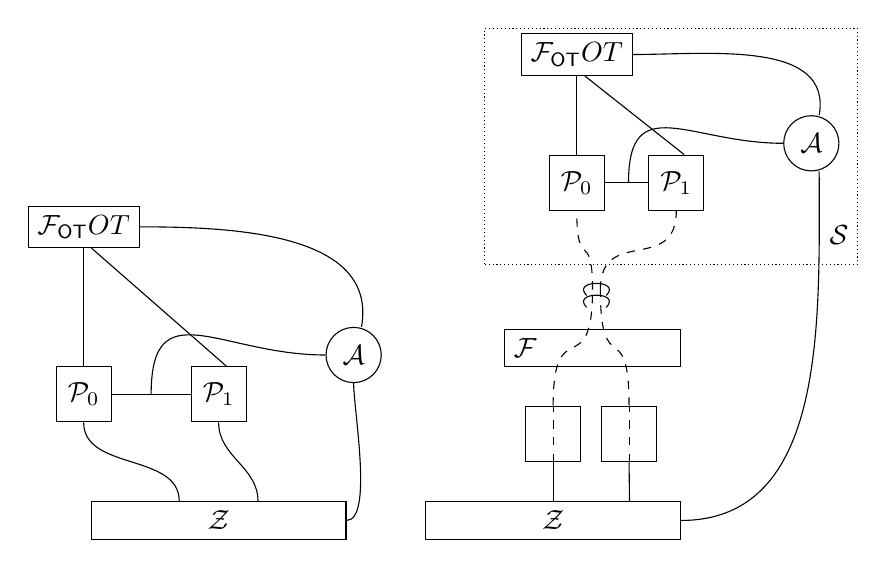
\begin{tikzpicture}[node distance=0.25cm]
  %left picture
  \node[rectangle,draw,fill=none] (flipake) {$\Fot$};
  \node[rectangle,draw,fill=none,minimum size=0.7cm] (pi) [below=1.5cm of flipake] {$\firstparty$};
  \node[rectangle,draw,fill=none,minimum size=0.7cm] (pj) [right=1cm of pi] {$\secondparty$};
  \node[circle,draw,fill=none] (adv) [right=1cm of pj,yshift=0.5cm] {\AdvA};
  \node[rectangle,draw,fill=none,text width=3cm,text centered] (env) [below=1cm of pj] {\Env};
  % from the parties to the helping functionalities
  \draw[-] (flipake.south) edge (pi.north);
  \draw[-] ([xshift=0.1cm] flipake.south) edge ([xshift=0.1cm] pj.north);
  % between parties
  \draw[-] (pi.east) edge (pj.west);
  % from environment to (honest) parties
  \draw[-] ([xshift=-0.5cm] env.north) edge[out=90,in=270] (pi.south);
  \draw[-] ([xshift=0.5cm] env.north) edge[out=90,in=270] (pj.south);
  % from environment to adversary
  \draw (env.east) edge[out=0,in=270,looseness=0.5] (adv.south);
  % the adversary controlling the channel
  \draw[-] ([xshift=0.5cm] pi.east) edge[out=90,in=180,looseness=1.5] (adv.west);
  % from adversary to helping functionalities
  \draw ([xshift=0.1cm] adv.north) edge[out=80,in=0] (flipake.east);
%   \coordinate (dotsleft) at ($(pi.west)$);
%     \draw [thick,dotted,-] ($(dotsleft)+(-0.2cm,0cm)$) -- ($(dotsleft)+(-0.5cm,0cm)$);
 
  %right picture
  \node[rectangle,draw,fill=none,text width=3cm,text centered] (env1) [right=1cm of env] {$\Env$};
  \node[rectangle,draw,fill=none,minimum size=0.7cm] (dpi) [above=0.5cm of env1] {};
  \node[rectangle,draw,fill=none,minimum size=0.7cm] (dpj) [right=of dpi] {};
  \node[rectangle,draw,fill=none,text width=2cm] (f) [above=1.7cm of env1,xshift=0.5cm] {$\Func$};
  
  %simulator's box
  \node[rectangle,draw,fill=none,densely dotted,minimum width=4.5cm,minimum height=3cm,
   text width=4.5cm,text height=2.5cm,align=right] (sbox) [above=3cm of env1,xshift=1.5cm] {$\Sim$}; %dotted box % \SimYGCRFE
  \node[rectangle,draw,fill=none,minimum size=0.7cm] (spi) [above=1.5cm of f,xshift=-0.2cm] {$\firstparty$};
  \node[rectangle,draw,fill=none,minimum size=0.7cm] (spj) [right=of spi,xshift=0.3cm] {$\secondparty$};
  \node[rectangle,draw,fill=none] (fot) [above=1cm of spi]{$\Fot$}; 
  \node[circle,draw,fill=none] (sadv) [right=1cm of spj,yshift=0.5cm] {$\AdvA$};
  % wires from the parties to the helping functionalities
  \draw[-] (fot.south) edge (spi.north);
  \draw[-] ([xshift=0.1cm] fot.south) edge ([xshift=0.1cm] spj.north);
  % wires between parties
  \draw[-] (spi.east) edge (spj.west);
  % wires from environment to adversary
  \draw[-] ([xshift=0.1cm]sadv.south) edge[out=270,in=0] (env1.east);
  % the adversary controlling the channel
  \draw[-] ([xshift=0.3cm] spi.east) edge[out=90,in=180,looseness=1.5] (sadv.west);
  % wires from adversary to helping functionalities
  \draw ([xshift=0.1cm] sadv.north) edge[out=80,in=0] (fot.east);
  
  % wires outside the simulator
  \draw[-] (dpj.south) edge[dashed] (dpj.north); %inside dummy party Pj
  \draw[-] (dpi.south) edge[dashed] (dpi.north); %inside dummy party Pi
  \node (mergepoint) [above=0.5cm of f] {}; %dummy node for mergepoint
  \draw[-] (dpj.north) edge[dashed,out=90,in=270,looseness=2] ([xshift=0.1cm]mergepoint.south); % the two merged wires, lower part
  \draw[-] (dpi.north) edge[dashed,out=90,in=270,looseness=2] (mergepoint.south);
  \draw[-] ([xshift=0.1cm]mergepoint.south) edge[dashed,out=90,in=270,looseness=1.5] (spj.south); %upper part
  \draw[-] (mergepoint.south) edge[dashed,out=90,in=270,looseness=2] (spi.south);
  \draw[-] ([yshift=-0.2cm,xshift=0.05cm]mergepoint.east) edge[looseness=3] ([yshift=-0.2cm,xshift=0.05cm]mergepoint.west); % the curve tying the wires together
  \draw[-] ([yshift=-0.35cm,xshift=0.05cm]mergepoint.east) edge[looseness=3] ([yshift=-0.35cm,xshift=0.05cm]mergepoint.west);
  \draw[-] (env1.north) edge (dpi.south);
  \draw[-] ([xshift=0.97cm] env1.north) edge (dpj.south);
\end{tikzpicture}
 \caption{Transition from game~\printgame{real} (left) to game~\printgame{layout} (right), showing a setting where both parties are honest.}
 \label{fig:g0g1layout}
\end{figure}

\game{YGCRFEbuildF}
\textbf{Adding $\Func$'s Record-Keeping and $\TestPwd$ Interface}


\textit{Modifications to $\Func$:}
We now allow $\Func$ to do all of the record-keeping described in Figure~\ref{fig:func-RFE}.

$\Func$ still forwards $\NewSession$ queries from the dummy parties in their entirety (including the \password) to $\SimYGCRFE$, but also records them.
Since this is a matter of internal record-keeping only, this does not affect $\AdvA$'s view.

\textit{Modifications to $\SimYGCRFE$:}
$\SimYGCRFE$ creates $\NewKey$ queries for $\Func$ from whatever output the simulated parties produce. 
In this game, $\Func$ still simply forwards the keys it is given to the dummy parties without modifying them, so this does not affect $\AdvA$'s view.
\julia[inline]{Since, technically, modification of $\SimYGCRFE$ might change the output behaviour of $\Func$, you should first change $\Func$ and $\Sim$ and afterwards argue indistinguishability.}
\sophia[inline]{Yeah, we combined two very minor changes into one game, but since they're so superficial I don't think it matters...}

\game{YGCRFEkeyshonestclose}
\textbf{Allowing $\Func$ to Choose Keys For Two Honest Parties With Close \Passwords}

\textit{Modifications to $\Func$:}
We now allow $\Func$ to follow the instructions in Figure~\ref{fig:func-RFE} to choose the key when $\firstparty$ and $\secondparty$ are both honest, and $d(\firstpw, \secondpw) \leq \delta$.

We can use any environment who can distinguish this game from Game~\previousgame to build an adversary $\AdvB$ that can break the garbled output randomness property (Definition~\ref{def:garbledoutputrandomness}, Theorem~\ref{theorem:garbledoutputrandomness}) of our garbling scheme.

\julia[inline]{I do not manage to fully follow the proof of this, that's why instead I just ask a question: in this game, you change \Func such that it either chooses a fresh random key for an honest session with close \passwords OR aligns the key if there already was one for this session. For the second case, the proof of indistinguishability should require the correctness of the protocol. Why don't you need that?}
\sophia[inline]{It only requires the correctness of the protocol in this one case, where both parties are honest and their inputs are close. We use it implicitly - the two outputs will be XORs of the same values.}
Since both parties are honest, in order to use the environment as a distinguisher, the adversary needs to give the environment a transcript of the parties' interactions ($\gfunc_{\firstindex}, \ginp_{\firstindex,\firstindex}, \gfunc_{\secondindex}, \ginp_{\secondindex,\secondindex}$) as well as the parties' output keys.
Because we are in the OT hybrid model, the environment sees neither inputs to the OT nor its outputs.

Our adversary $\AdvB$ executes $\SimYGCRFE$'s simulation of $\firstparty$ with the $\Func$ of Game~\previousgame with some modifications.
First, it finds a \password $\pw$ such that $d(\firstpw, \pw) > \delta$.
(Note that in order for this reduction to work, such a \password must be efficiently computable, which it is by the assumption in the statement of Theorem~\ref{theorem:YGCRFE}.)
Instead of running $\gb$, $\AdvB$ queries the garbled output randomness challenger on $(\func, (\firstpw, \pw))$ to obtain $(\gfunc_{\firstindex}, \ginp_{\firstindex}, \random)$.
Let $\ginp_{\firstindex} = (\ginp_{\firstindex, \firstindex}, \ginp_{\firstindex, \secondindex})$.
Note that $\gfunc_{\firstindex}$ and $\ginp_{\firstindex,\firstindex}$ are generated by the challenger exactly as they would be by $\SimYGCRFE$, so those values do not change. 
($\ginp_{\firstindex,\secondindex}$ is different, since $\pw$ is different from $\secondpw$, but $\ginp_{\firstindex,\secondindex}$ is not visible to the environment.)
Since the adversary used a \password $\pw$ that is dissimilar to $\secondpw$, it uses the value $\random$ --- corresponding to the output label \emph{not} returned by $\ev(\gfunc_{\firstindex}, \ginp_{\firstindex})$ --- as $\key_{\firstindex, correct}$.
($\ev(\gfunc_{\firstindex}, \ginp_{\firstindex})$ would give $\key_{\firstindex, wrong}$.) 
If $b = 0$, the challenger will return the actual $\key_{\firstindex, correct}$ as $\random$, and the environment's view will be that of Game~\previousgame.
If $b = 1$, the challenger will give a random value as $\random$.
If $\random$ is truly random, then so is $\random \oplus \goutp_{\secondindex}$; so, the environment's view will be that of Game~\thisgame.
(Note that we do not change the way in which $\secondparty$ generates $\gfunc_{\secondindex}, \ginp_{\secondindex}$, but we do set $\secondparty$'s output key to be the same as $\firstparty$'s. 
This will be the key that an honest execution of the protocol would produce if $b = 0$, and random otherwise.)
The adversary $\AdvB$ then returns the environment's guess as $b'$.
The advantage of $\AdvB$ in the garbled output randomness game will be exactly the same as that of the environment in distinguishing between Game~\previousgame and Game~\thisgame.

\game{YGCRFEkeyshonestfarone}
\textbf{Allowing $\Func$ to Choose Keys For One of Two Honest Parties With Dissimilar \Passwords}

\textit{Modifications to $\Func$:}
We now allow $\Func$ to follow the instructions in Figure~\ref{fig:func-RFE} to choose the key for $\firstparty$ when $\firstparty$ and $\secondparty$ are both honest, and $d(\firstpw, \secondpw) > \delta$.
\julia[inline]{This includes the case where one party already got a key? Or do you assume that $\firstparty$ always gets the output first?}
\sophia[inline]{Order does not matter here - so, it covers both the case where $\secondparty$ already got their key, and the case where they didn't.}

We can use any environment who can distinguish this game from Game~\previousgame to build an adversary $\AdvB$ that can break the garbled output randomness property (Definition~\ref{def:garbledoutputrandomness}, Theorem~\ref{theorem:garbledoutputrandomness}) of our garbling scheme.

Our adversary $\AdvB$ executes $\SimYGCRFE$'s simulation of $\firstparty$ with the $\Func$ of Game~\previousgame with some modifications.
Instead of running $\gb$, $\AdvB$ queries the garbled output randomness challenger on $(\func, (\firstpw, \secondpw))$ to obtain $(\gfunc_{\firstindex}, \ginp_{\firstindex}, \random)$.
Note that $\gfunc_{\firstindex}$ and $\ginp_{\firstindex}$ are generated by the challenger exactly as they would be by $\SimYGCRFE$, so these values do not change. 
If $b = 0$, the challenger will return the actual $\key_{\firstindex, correct}$ as $\random$, and the environment's view will be that of Game~\previousgame.
If $b = 1$, the challenger will give a random value as $\random$.
If $\random$ is truly random, then so is $\random \oplus \goutp_{\secondindex}$; so, the environment's view will be that of Game~\thisgame.
The adversary $\AdvB$ then returns the environment's guess as $b'$.
The advantage of $\AdvB$ in the garbled output randomness game will be exactly the same as that of the environment in distinguishing between Game~\previousgame and Game~\thisgame.

\game{YGCRFEkeyshonestfartwo}
\textbf{Allowing $\Func$ to Choose Keys For Both Honest Parties With Dissimilar \Passwords}

\textit{Modifications to $\Func$:}
We now allow $\Func$ to follow the instructions in Figure~\ref{fig:func-RFE} to choose the key for $\secondparty$ as well as for $\firstparty$ when $\firstparty$ and $\secondparty$ are both honest, and $d(\firstpw, \secondpw) > \delta$.

We can use any environment who can distinguish this game from Game~\previousgame to build an adversary that can break the garbled output randomness property (Definition~\ref{def:garbledoutputrandomness}, Theorem~\ref{theorem:garbledoutputrandomness}) of our garbling scheme, exactly as we did in the reduction above.

\game{YGCRFEtwohonesthybrid}
\textbf{Simulating $\gfunc, \ginp$ for One of Two Honest Parties}

\textit{Modifications to $\SimYGCRFE$:}
Consider the case when both $\firstparty$ and $\secondparty$ are honest.
In this game, the simulator replaces $\firstparty$'s garbled circuit and input with simulated ones.
$\SimYGCRFE$ does not need to simulate anything relating to the OT, since the environment cannot observe OT functionality inputs or outputs if both participating parties are honest.
$\SimYGCRFE$ uses the obliviousness simulator to generate $\gfunc_{\firstindex}, \ginp_{\firstindex}$ (while continuing to generate $\gfunc_{\secondindex}, \ginp_{\secondindex}$ honestly), and sends the garbled circuits and the appropriate parts of the garbled inputs between the parties.
$\SimYGCRFE$ outputs $\bot$ bot as both parties' keys, since the outputs don't matter - $\Func$ takes care of outputting appropriate keys as of a few games ago (Game~\printgame{YGCRFEkeyshonestclose} if $d(\firstpw, \secondpw) \leq \delta$, and Games~\printgame{YGCRFEkeyshonestfarone},\printgame{YGCRFEkeyshonestfartwo} otherwise), so this change is not observable by the environment.

We can use any environment who can distinguish this game from Game~\previousgame to build an adversary $\AdvB$ that can break the obliviousness property %(Definition~\ref{def:obliviousness}) 
of our garbling scheme.
$\AdvB$ executes $\SimYGCRFE$'s simulation of $\firstparty$ as in Game~\previousgame, but instead of generating $(\gfunc_{\firstindex}, \ginp_{\firstindex})$ and $(\gfunc_{\secondindex}, \ginp_{\secondindex})$ according to the protocol, it queries the obliviousness challenger on $(\func, (\firstpw, \secondpw))$ to obtain $(\gfunc_{\firstindex}, \ginp_{\firstindex})$.
If $b = 0$, the challenger will return actual $(\gfunc_i, \ginp_i)$ values, and the environment's view we will be that of Game~\previousgame.
If $b = 1$, the challenger will return simulated values, and the environment's view will be that of this game.
The adversary $\AdvB$ then returns the environment's guess as $b'$.
The advantage of $\AdvB$ in the obliviousness game will be exactly the same as that of the environment in distinguishing between Game~\previousgame and Game~\thisgame.

\game{YGCRFEtwohonest}
\textbf{Removing \Password Forwarding Always}

\textit{Modifications to $\Func$:}
We now modify $\Func$ to forward only $(\NewSession, \sid, \aparty)$ to $\SimYGCRFE$ (omitting the \password $\apw$) for $\aparty \in \{\firstparty, \secondparty\}$ when $\firstparty$ and $\secondparty$ are both honest. 

\textit{Modifications to $\SimYGCRFE$:}
In Game~\previousgame, $\SimYGCRFE$ started simulating $\firstparty$'s messages without using knowledge of $\firstpw$.
$\SimYGCRFE$ now also simulates $\secondparty$'s messages by using the obliviousness simulator to generate the garbled circuit and input $\gfunc_{\secondindex}, \ginp_{\secondindex}$.

We can use any environment who can distinguish this game from Game~\previousgame to build an adversary $\AdvB$ that can break the obliviousness property %(Definition~\ref{def:obliviousness}) 
of our garbling scheme.
$\AdvB$ executes $\SimYGCRFE$'s simulation of $\secondparty$ as in Game~\previousgame, but instead of generating $(\gfunc_{\secondindex}, \ginp_{\secondindex})$ according to the protocol, it queries the obliviousness challenger on $(\func, (\secondpw, \firstpw))$ to obtain $(\gfunc_{\secondindex}, \ginp_{\secondindex})$.
If $b = 0$, the challenger will return actual $(\gfunc_{\secondindex}, \ginp_{\secondindex})$ values, and the environment's view we will be that of Game~\previousgame.
If $b = 1$, the challenger will return simulated values, and the environment's view will be that of this game.
The adversary $\AdvB$ then returns the environment's guess as $b'$.
The advantage of $\AdvB$ in the obliviousness game will be exactly the same as that of the environment in distinguishing between Game~\previousgame and Game~\thisgame.

\game{YGCRFEresetmaliciousinput}
\textbf{Setting the Malicious Input as in the ``Standard Corruption Model''}

\textit{Modifications to $\SimYGCRFE$:}
In this game, $\SimYGCRFE$ sets a corrupt party $\otherparty$'s $\NewSession$ input according to the standard corruption model~\cite{FOCS:Canetti01}.
It does so as soon as it sees $\otherpw'$, when it is given as an input to the ideal OT functionality. 
Since $\Func$ does not currently use $\otherpw$, this does not affect the environment's view.

\game{YGCRFEkeyscorrupt}
\textbf{Allowing $\Func$ to Choose the Key For An Honest Party With a \Password Dissimilar to Its Corrupt Partners'}

\textit{Modifications to $\Func$:}
We now allow $\Func$ to follow the instructions in Figure~\ref{fig:func-RFE} to choose all keys.
Note that the only remaining scenario this affects is the one where only one party $\aparty \in \{\firstparty, \secondparty\}$ is honest, and $d(\firstpw, \secondpw) > \delta$.
If both parties are corrupt, or if only one party is corrupt and $d(\firstpw, \secondpw) \leq \delta$, $\Func$ still simply forwards the output key.

We can use any environment who can distinguish this game from Game~\previousgame to build an adversary $\AdvB$ that can break the garbled output randomness property (Definition~\ref{def:garbledoutputrandomness}, Theorem~\ref{theorem:garbledoutputrandomness}) of our garbling scheme.
Our adversary $\AdvB$ executes $\SimYGCRFE$'s simulation of $\firstparty$ with the $\Func$ of Game~\previousgame with some modifications.
Instead of running $\gb$ first, it waits to see $\otherparty$'s input $\otherpw'$ to the ideal OT functionality, and then queries the garbled output randomness challenger on $(\func, (\apw, \otherpw'))$ to obtain $(\gfunc_{\aindex}, \ginp_{\aindex}, \random)$.
Note that $\gfunc_{\aindex}$ and $\ginp_{\aindex}$ are generated by the challenger exactly as they would be by $\SimYGCRFE$, so those values do not change. 
The adversary then uses $\random$ as $\key_{\aindex, correct}$.
If $b = 0$, the challenger will return the actual $\key_{\aindex, correct}$ as $\random$, and the environment's view will be that of Game~\previousgame.
If $b = 1$, the challenger will give a random value as $\random$.
If $\random$ is truly random, then so is $\random \oplus \goutp_{\otherindex}$; so, the environment's view will be that of Game~\thisgame.
The adversary $\AdvB$ then returns the environment's guess as $b'$.
The advantage of $\AdvB$ in the garbled output randomness game will be exactly the same as that of the environment in distinguishing between Game~\previousgame and Game~\thisgame.

\game{YGCRFEsimulatedgfuncginp}
\textbf{Simulating Garbled Circuit and Inputs For An Honest Party With a Corrupt Partner}

\textit{Modifications to $\SimYGCRFE$:}
In this game, $\SimYGCRFE$ simulates $\gfunc_{\aindex}$ and $\ginp_{\aindex}$ when $\aparty$ is honest and $\otherparty$ is corrupt. 

In more detail, $\SimYGCRFE$ proceeds as follows on behalf of $\aparty$:

\begin{itemize}
\item
$\SimYGCRFE$ postpones step 1.
\item 
In step 2, $\SimYGCRFE$:
\begin{itemize}
\item Plays an OT sender as follows:
\begin{itemize}
\item Waits for $\otherparty$ to provide their select bits to the OT.
As a result, $\SimYGCRFE$ learns the \password used by $\otherparty$, $\otherpw'$.
\item If $d(\apw, \otherpw') \leq \delta$ sets $\outp = 1$, and sets $\outp = 0$ otherwise.
\item Uses the privacy simulator for the garbling scheme to generate \linebreak $(\gfunc_{\aindex}, \ginp_{\aindex}, \deinp_{\aindex}) \gets \simulator(1^{\secparam}, \func, \outp)$.
\item Parses $(\ginp_{\aindex,\aindex}, \ginp_{\aindex,\otherindex}) \gets \ginp_{\aindex}$.
\item Sends $\ginp_{\aindex,\otherindex}$ to $\otherparty$ as the OT output.
\end{itemize}
\item Plays an OT receiver honestly.
\end{itemize}
\item 
$\SimYGCRFE$ follows the instructions in Figure~\ref{fig:YGCRFE} for steps 3-8.
\end{itemize}

We can use any environment who can distinguish this game from Game~\previousgame to build an adversary $\AdvB$ that can break the privacy property %(Definition~\ref{def:privacy}) 
of our garbling scheme.
Our adversary $\AdvB$ executes $\SimYGCRFE$'s simulation of $\firstparty$ with some modifications.
Instead of running the privacy simulator $\simulator$, it queries the privacy challenger on $(\func, (\apw, \otherpw'))$ to obtain $(\gfunc_{\aindex}, \ginp_{\aindex}, \deinp_{\aindex})$.
If $b = 0$, the challenger will return actual $(\gfunc_{\aindex}, \ginp_{\aindex}, \deinp_{\aindex})$ values, and the environment's view will be that of Game~\previousgame; if $b = 1$, the challenger return simulated values, and the environment's view will be that of this game.
The adversary $\AdvB$ then returns the environment's guess as $b'$.
The advantage of $\AdvB$ in the privacy game will be exactly the same as that of the environment in distinguishing between Game~\previousgame and Game~\thisgame.

\game{YGCRFEonehonest}
\textbf{Removing \Password Forwarding To An Honest Party With a Corrupt Partner}

\textit{Modifications to $\Func$:}
%We now modify $\Func$ as follows: 
\begin{itemize}
\item
If $\aparty$ is honest and $\otherparty$ is corrupt, then, upon receiving a $\NewSession$ query, $\Func$ forwards only $(\NewSession, \allowbreak \sid, \aparty)$ to $\SimYGCRFE$ (omitting the \password $\apw$).
\item
$\Func$ now processes $\TestPwd$ queries (which were not issued in any prior game) according to the instructions in Figure~\ref{fig:func-RFE}. 
Given a $(\TestPwd, \sid, \aparty)$ query ($\aparty \in \{\firstparty, \secondparty\}$),
if $d(\firstpw, \secondpw) \leq \delta$, $\Func$ sends $\apw$ to $\SimYGCRFE$.
%(We do not consider $\delta \leq d(\firstpw, \secondpw) < \gamma$, since this construction has $\delta = \gamma$.)
\end{itemize}

\textit{Modifications to $\SimYGCRFE$:}
Now that $\SimYGCRFE$ does not know $\aparty$'s \password, it must simulate the honest party's messages without that knowledge.

In more detail, $\SimYGCRFE$ proceeds as follows on behalf of $\aparty$:

\begin{itemize}
\item
$\SimYGCRFE$ postpones step 1.
\item 
In step 2, $\SimYGCRFE$:
\begin{itemize}
\item Plays an OT sender as follows:
\begin{itemize}
\item As in Game~\printgame{YGCRFEsimulatedgfuncginp}, waits for $\otherparty$ to provide their select bits to the OT.
As a result, $\SimYGCRFE$ learns the \password used by $\otherparty$, $\otherpw'$.
\item Makes a $(\TestPwd, \sid, \Party_i)$ query to $\Func$. 
If $d(\apw, \otherpw') \leq \delta$ (that is, the adversary has approximately guessed $\aparty$'s \password), $\SimYGCRFE$ learns $\apw$, and sets $\apw' = \apw$.
Otherwise, it sets $\apw'$ at random such that $d(\apw', \otherpw') > \delta$, and uses $\apw'$ in place of $\apw$ in the rest of the simulation.
\item As in Game~\printgame{YGCRFEsimulatedgfuncginp}, If $d(\apw, \otherpw') \leq \delta$ sets $\outp = 1$, and sets $\outp = 0$ otherwise.
\item As in Game~\printgame{YGCRFEsimulatedgfuncginp}, uses the privacy simulator for the garbling scheme to generate $(\gfunc_{\aindex}, \ginp_{\aindex}, \deinp_{\aindex}) \gets \simulator(1^{\secparam}, \func, \outp)$.
\item As in Game~\printgame{YGCRFEsimulatedgfuncginp}, parses $(\ginp_{\aindex,\aindex}, \ginp_{\aindex,\otherindex}) \gets \ginp_{\aindex}$.
\item As in Game~\printgame{YGCRFEsimulatedgfuncginp}, sends $\ginp_{\aindex,\otherindex}$ to $\otherparty$ as the OT output.
\end{itemize}
\item Plays an OT receiver honestly with $\apw'$.
\end{itemize}
\item 
$\SimYGCRFE$ follows the instructions in Figure~\ref{fig:YGCRFE} for steps 3-8.
\end{itemize}

%\begin{itemize}
%\item 
%$\SimYGCRFE$ makes a $(\TestPwd, \sid, \Party_i)$ query to $\Func$. 
%If $d(\pw_i, \pw_j') < \delta$ (that is, the adversary has approximately guessed $\Party_i$'s \password), $\SimYGCRFE$ learns $\pw_i$, and sets $\pw_i' = \pw_i$.
%Otherwise, it sets $\pw_i'$ at random such that $d(\pw_i', \pw_j') \geq \delta$, and uses $\pw_i'$ in place of $\pw_i$ in the rest of the simulation.
%\item
%$\SimYGCRFE$ executes the rest of the simulation as in Game~\previousgame.
%Note that thanks to its query to $\TestPwd$, $\SimYGCRFE$ knows everything it needs to in order to play the OT sender as described in Game~\previousgame.
%\end{itemize}

Nothing could have changed from the point of view of \Env.
If $d(\apw, \otherpw') \leq \delta$, this game is identical to Game~\previousgame.
If $d(\apw, \otherpw') > \delta$, a random $\apw'$ is used instead of $\apw$.
However, $\apw'$ only affects the OT execution with $\aparty$ as receiver, where $\otherparty$ does not receive any outputs anyway.
In this case, $\aparty$'s output key gets set randomly by $\Func$ as of Game~\printgame{YGCRFEkeyscorrupt}, so that does not change.

\end{games}

In Figure~\ref{fig:SimulatorYGCRFE}, we show the simulator $\SimYGCRFE$ for $\Prfe$.

\begin{figure}[!ht]
\noindent
\scriptsize
\fbox{\begin{minipage}{\linewidth-10pt}
\begin{itemize}
\item 
Upon receiving $(\NewSession, \sid, \aparty)$ from $\Frfe^{P}$ for honest party $\aparty$ when $\otherparty$ is also honest, $\SimYGCRFE$ generates $\gfunc_{\aindex}, \ginp_{\otherindex}$ using the obliviousness simulator for the garbling scheme, and sends those to $\otherparty$.
\item 
Upon receiving $(\NewSession, \sid, \aparty)$ from $\Frfe^{P}$ for honest party $\aparty$ when $\otherparty$ is corrupt, $\SimYGCRFE$ does the following:
\begin{itemize}
\item
$\SimYGCRFE$ postpones step 1.
\item 
In step 2, $\SimYGCRFE$:
\begin{itemize}
\item Plays an OT sender as follows:
\begin{itemize}
\item Waits for $\otherparty$ to provide their select bits to the OT.
As a result, $\SimYGCRFE$ learns the \password used by $\otherparty$, $\otherpw'$.
%\item Sends $\otherpw'$ to $\Func$ as $\otherparty$'s updated $\NewSession$ input, as part of the ``standard corruption'' model.
\item Makes a $(\TestPwd, \sid, \Party_i)$ query to $\Func$. 
If $d(\apw, \otherpw') \leq \delta$ (that is, the adversary has approximately guessed $\aparty$'s \password), $\SimYGCRFE$ learns $\apw$, and sets $\apw' = \apw$.
Otherwise, it sets $\apw'$ at random such that $d(\apw', \otherpw') > \delta$, and uses $\apw'$ in place of $\apw$ in the rest of the simulation.
\item If $d(\apw, \otherpw') \leq \delta$ sets $\outp = 1$, and sets $\outp = 0$ otherwise.
\item Uses the privacy simulator for the garbling scheme to generate $(\gfunc_{\aindex}, \ginp_{\aindex}, \deinp_{\aindex}) \gets \simulator(1^{\secparam}, \func, \outp)$.
\item Parses $(\ginp_{\aindex,\aindex}, \ginp_{\aindex,\otherindex}) \gets \ginp_{\aindex}$.
\item Sends $\ginp_{\aindex,\otherindex}$ to $\otherparty$ as the OT output.
\end{itemize}
\item Plays an OT receiver honestly with $\apw'$.
\end{itemize}
\item 
$\SimYGCRFE$ follows the instructions in Figure~\ref{fig:YGCRFE} for steps 3-8 with $\pw_i'$.
\end{itemize}
\end{itemize}
Additionally, $\SimYGCRFE$ forwards all other instructions from \Env to \AdvA and reports all output of \AdvA towards \Env. Instructions of corrupting a player are only obeyed if they are received before the protocol started, i.e., before \Sim received any \NewSession query from $\Frfe^{P}$.
\end{minipage}}
\caption{Simulator $\SimYGCRFE$ for $\Prfe$} 
\label{fig:SimulatorYGCRFE}
\end{figure}

% !TEX root = ../main.tex
% !TEX spellcheck = en-US

\section{Proof that $\Fsrfe^{P}$ is Enough to Realize $\FFAKE^{P}$}
\label{sec:ygcfakeproof}

In Figure~\ref{fig:YGCFAKE}, we describe a protocol $\PfakeYGC$ which trivially realizes $\FFAKE^{P}$ in the $\Fsrfe^{P}$-hybrid model.
\leo[inline]{Out of curiousity (and to help the reader), would be correct to say  ``$\Fsrfe^{P}$ is essentially the same as $\FFAKE^{P}$, and any protocol that realizes one also realizes the other?''}

\julia[inline]{$\PfakeYGC$ has nothing to do with YGC, so the name is a bit misleading. If someone later references the theorem this might be confusing.}

\begin{figure}[htbp]
  \centering
  \begin{fboxenv}
    \begin{minipage}{0.95\textwidth}
    	Upon receiving the input $(\sid, \apw)$, $\aparty \in \{\firstparty, \secondparty\}$ does the following:
	\begin{itemize}
	\item Sends $(\Init, \sid)$ to $\Fsrfe^{P}$;
	\item Sends $(\NewSession, \sid, \apw)$ to $\Fsrfe^{P}$;
	\item Waits for $\key$ from $\Fsrfe^{P}$, and 
	\item Outputs $\key$.
	\end{itemize}
    \end{minipage}
  \end{fboxenv}
  \caption{Protocol $\PfakeYGC$ realizing $\FFAKE^{P}$ in the $\Fsrfe^{P}$-hybrid model.}
  \label{fig:YGCFAKE}
\end{figure}

\begin{theorem}
Protocol $\PfakeYGC$ realizes $\FFAKE^{P}$ in the $\Fsrfe^{P}$-hybrid model.
\end{theorem}

\expl{Canetti~\etal~\cite{PKC:CDVW12} make a similar claim but only defend it in a ``full" version that is not available online.}

\begin{proof}
For every efficient adversary $\AdvA$, we describe a simulator $\SimYGCFAKE$ in Figure~\ref{fig:SimulatorYGCFAKE} such that no efficient environment can distinguish an execution with the real protocol $\PfakeYGC$ and $\AdvA$ from an execution with the ideal functionality $\FFAKE^{P}$ and $\SimYGCFAKE$.
Since the environment does not get any information about the honest parties except their output, all the simulator needs to do is respond to queries to $\Fsrfe^{P}$.
%$\SimYGCFAKE$ controls the ideal functionality $\Fsrfe^{P}$, so it can see all the adversarial inputs to that ideal functionality, but the adversary cannot see honest parties' inputs or outputs.
Since the honest party does nothing except query the ideal functionality $\Fsrfe^{P}$, and its output gets replaced by values chosen by $\FFAKE^{P}$, there is nothing to simulate.

\begin{figure}[htbp]
  \centering
  \begin{fboxenv}
    \begin{minipage}{0.95\textwidth}
    $\SimYGCFAKE$ responds to queries to $\Fsrfe^{P}$ as follows:
	\begin{itemize}
	\item Upon getting $(\Init, \sid)$ from $\AdvA$ on behalf of corrupt party $\otherparty \in \{\firstparty, \secondparty\}$, $\SimYGCFAKE$ 
	does nothing.
	%executes the code in Figure~\ref{fig:func-SRFE}.
	\item Upon getting $(\Init, \sid, \aparty, H, \sid_{H})$ from $\AdvA$, $\SimYGCFAKE$ 
	does nothing.
	%executes the code in Figure~\ref{fig:func-SRFE}.
	\item Upon getting $(\NewSession, \sid, \apw)$ from $\AdvA$ on behalf of honest party $\aparty \in \{\firstparty, \secondparty\}$, $\SimYGCFAKE$ does nothing.
	\item Upon getting $(\NewSession, \sid, \otherpw')$ from $\AdvA$ on behalf of corrupt party $\otherparty \in \{\firstparty, \secondparty\}$, $\SimYGCFAKE$:
	\begin{itemize}
	%\item Executes the code in Figure~\ref{fig:func-SRFE};
	\item Records $\otherpw'$;
	\item Sends $(\TestPwd, \sid, \aparty, \otherpw')$ to $\FFAKE^{P}$;
	\item If $d(\apw, \otherpw') \leq \delta$, $\SimYGCFAKE$ learns $\apw$.
	\end{itemize}
	\item Upon getting a $(\TestPwd, \sid, \aparty)$ query from $\AdvA$, 
	$\SimYGCFAKE$ responds with the output of the $\TestPwd$ query above.
	\item Upon getting a $(\NewKey, \sid, \aparty, \akey)$ query from $\AdvA$, 
	if $\aparty$ is corrupt, $\SimYGCFAKE$ outputs $\akey$ to $\aparty$.
	In any case, $\SimYGCFAKE$ forwards $(\NewKey, \sid, \aparty, \akey)$ to $\FFAKE^{P}$.
	\end{itemize}
	Additionally, $\SimYGCFAKE$ forwards all other instructions from \Env to \AdvA and reports all output of \AdvA towards \Env. Instructions of corrupting a player are only obeyed if they are received before the protocol started, i.e., before \Sim received any \NewKey query from $\FFAKE^{P}$.
    \end{minipage}
  \end{fboxenv}
  \caption{Simulator $\SimYGCFAKE$ for $\PfakeYGC$.}
  \label{fig:SimulatorYGCFAKE}
\end{figure}

All that remains to show is that the values produced by $\FFAKE^{P}$ and by $\Fsrfe^{P}$ are identically distributed.
We describe the outputs of $\FFAKE^{P}$ and $\Fsrfe^{P}$ in Figure~\ref{fig:outputtables}.
The table enumerates all possible cases in the functionalities. 
Cases in $\Fsrfe^{P}$ are described in terms of the distances between \passwords: between the honest parties' \passwords if no man in the middle attack occurred, and between adversarial and honest \passwords if it did.
(If the adversary engaged one party but not the other, only one of the distances is filled in.)
Cases in $\FFAKE^{P}$ are described in terms of record markings (``fresh'', ``compromised'' or ``interrupted'').
There is a one-to-one mapping between the cases in $\Fsrfe^{P}$ and $\FFAKE^{P}$ such that the outputs for the parties, whether they are honest or corrupt, are identically distributed.
Those outputs are described in the last three columns of the table, as tuples of values the first of which is output to $\firstparty$, and the second of which is output to $\secondparty$.
$a, b$ are adversarially chosen values (which may or may not be distinct).
$r, s$ are independent, uniformly random values.

%``(g, g)'' denotes the case where both parties are good; ``(g, b)'' denotes the case where $\Party_i$ is good and $\Party_j$ is bad; ``(b, g)'' denotes the reverse; and ``(b, b)'' denotes the case where both parties are bad.
%Outputs within the table are written as tuples of random and adversarially chosen values, where the first value is output to $\Party_i$, and the second to $\Party_j$.
%$a, b$ are adversarially chosen values (which may or may not be distinct).
%$r, s$ are independent, uniformly random values.
%``Close'' denotes the case where $d(\pw_i, \pw_j) \leq \delta$, and ``far'' denotes the case where $d(\pw_i, \pw_j) > \delta$.
%The first two rows represent the case where the two parties are not split up by a man in the middle (so, only one indicator of closeness is necessary), and the last eight rows represent the cases where they are. 
%``Close'' indicates that the the \passwords in the relevant session were sufficiently similar; ``far'' indicates that they were not.
%In the case where the adversary split the two parties, $\bot$ indicates the adversary failed to engage in one of the two sessions.
%``(Close, close)'' then denotes the case that the man in the middle guessed sufficiently close \passwords in both sessions, and so on.

\begin{figure}
\centering

\scriptsize

%\begin{tabular}{|c||c|c|c|c|}
%\hline
%$\Frfe^{P}$ & (g, g) & (g, b) & (b, g) & (b, b) \\ \hline \hline
%close & r, r & a, b & a, b & a, b \\ \hline
%far & r, s & r, b & a, s & a, b  \\ \hline
%\end{tabular}

%\begin{tabular}{|c||c|c|c|c|}
%\hline
%$\Fsrfe^{P} = \FFAKE^{P}$ & (g, g) & (g, b) & (b, g) & (b, b) \\ \hline \hline
%close = (fresh, fresh) & r, r & a, b & a, b & a, b \\ \hline
%far = (fresh, fresh) & r, s & r, b & a, s & a, b  \\ \hline
%($\bot$, close) = (fresh, compromised) & r, b & r, b & a, b & a, b  \\ \hline
%($\bot$, far) = (fresh, interrupted) & r, s & r, b & a, s & a, b  \\ \hline
%(close, close) = (compromised, compromised) & a, b & a, b & a, b & a, b  \\ \hline
%(close, far) = (compromised, interrupted) & a, s & a, b & a, s & a, b  \\ \hline
%(close, $\bot$) = (compromised, fresh) & a, s & a, b & a, s & a, b \\ \hline
%(far, close) = (interrupted, compromised) & r, b & r, b & a, b & a, b  \\ \hline
%(far, far) = (interrupted, interrupted) & r, s & r, b & a, s & a, b  \\ \hline
%(far, $\bot$) = (interrupted, fresh) & r, s & r, b & a, s & a, b  \\ \hline
%\end{tabular}

\begin{tabular}{|C{2cm}|C{2cm}|C{2cm}||C{1.5cm}|C{1.5cm}||C{1cm}|C{1cm}|C{1cm}|}
\hline
\multicolumn{3}{|c||}{$\Fsrfe^{P}$} & \multicolumn{2}{c||}{$\FFAKE^{P}$} & \multicolumn{3}{C{3cm}|}{outputs in both $\Fsrfe^{P}$ and $\FFAKE^{P}$} \\ \hline
distance between $\firstparty$'s \password and $\secondparty$'s \password $d(\firstpw, \secondpw)$, if MITM didn't happen & distance between $\firstparty$'s \password and the adversary's $d(\firstpw, \secondpw')$, if MITM happened & distance between $\secondparty$'s \password and the adversary's $d(\firstpw', \secondpw)$, if MITM happened & $\firstparty$'s record & $\secondparty$'s record & $\firstparty$ and $\secondparty$ honest & $\firstparty$ honest, $\secondparty$ corrupt & $\firstparty$ and $\secondparty$ corrupt \\ \hline \hline
close ($\leq \delta$) & & & fresh & fresh & r, r & a, b & a, b \\ \hline
far ($> \delta$) & & & fresh & fresh & r, s & r, b & a, b \\ \hline \hline
& close ($\leq \delta$) & close ($\leq \delta$) & compromised & compromised & a, b & a, b & a, b  \\ \hline
& close ($\leq \delta$) & far ($> \delta$) & compromised & interrupted & a, s & a, b & a, b  \\ \hline
& close ($\leq \delta$) & & compromised & fresh & a, s & a, b & a, b \\ \hline
& far ($> \delta$) & close ($\leq \delta$) & interrupted & compromised & r, b & r, b & a, b  \\ \hline
& far ($> \delta$) & far ($> \delta$) & interrupted & interrupted & r, s & r, b & a, b  \\ \hline
& far ($> \delta$) & & interrupted & fresh & r, s & r, b & a, b  \\ \hline
& & close ($\leq \delta$) & fresh & compromised & r, b & r, b & a, b  \\ \hline
& & far ($> \delta$) & fresh & interrupted & r, s & r, b & a, b  \\ \hline
\end{tabular}

\caption{Output tables for %$\Frfe^{P}$ and 
$\FFAKE^{P}$ and $\Fsrfe^{P}$. $r, s$ represent random outputs, while $a, b$ represent adversarially chosen outputs.}
\label{fig:outputtables}
\end{figure}

\end{proof}

The transformation of Barak~\etal proceeds in two steps.
First, links are initialized:
\begin{enumerate}
\item
Each party generates a signing and verification key pair, and sends the verification key to its partner. 
\item 
Each party then signs the key it receives and sends the signature back.
\item
Each party verifies the signature it receives on its own verification key using the verification key it received; if the signature does not verify, it aborts.
\end{enumerate}
Second, the parties run the protocol exactly as they would over authenticated channels, signing each message with their signing key, and verifying each signature they receive.

Applying this transformation adds (1) two rounds of communication, and (2) a hash operation and a signature operation for each message, assuming the hash-and-sign paradigm is used.


% !TEX root = ../main.tex
% !TEX spellcheck = en-US

\section{A Concrete OT}

In this section, we recall a concrete UC-secure oblivious transfer protocol due to Chou and Orlandi~\cite{LC:ChoOrl15}.
While they consider the general case of $1$-out-of-$n$ transfer, we only consider $n = 2$.
Say $m$ $1$-out-of-$2$ OTs are performed.
The protocol requires the sender to compute $m +2$ exponentiations, and the receiver to compute $2m$ exponentiations, for a total of $3m + 2$ exponentiations.
\sophia[inline]{The statement in the abstract of Chou and Orlandi~\cite{LC:ChoOrl15} is inconsistent}
Figure~\ref{fig:concreteOT} shows a summary of the protocol.
Note that this construction does require a random oracle.

\begin{figure}
  \centering
   \begin{fboxenv}
     \begin{tabular}{rrcl}
     & Sender $\sender$ &   & Receiver $\receiver$ \\ \hline \\
     & $a \getsr \Z_p$ & & \\
     & $A = g^a$ & $\Rflow{A}$& \\
     & $T = A^a$ & & \\
     \multicolumn{1}{r}{\ldelim\{{7}{15mm}[$m$ times]} & let $M_0, M_1$ be the & & let $c \in \{0, 1\}$ be the \\
     & current messages & & current choice bit \\
     & & & $b \getsr \Z_p$ \\
     & & $\Lflow{B}$ & $B = A^cg^b$ \\
     &$\key_0 = H(A, B, B^a)$ & & $\key_{c} = H(A, B, A^b)$ \\
     &$\key_1 = H(A, B, B^a/T)$ & & \\
     &$e_0 \gets E_{k_0}(M_0)$ & & \\
     &$e_1 \gets E_{k_1}(M_1)$ & & \\
     && $\Rflow{e_0, e_1}{}$ & \\
     && & $M_c = D_{k_R}(e_c)$ \\
    \end{tabular}
   \end{fboxenv}
  \caption{A Concrete OT~\cite{LC:ChoOrl15} to be used in $\Prfe$}
  \label{fig:concreteOT}
\end{figure}

\expl{Note that the last step only seems necessary when specific messages are considered. Can we cut out a message step by using the keys $\key_0$ and $\key_1$ as the garbled circuit labels directly?}


\section{Proof of Theorem~\ref{theorem:lipake}}
\label{app:lipake}
% !TEX root = ../main.tex
% !TEX spellcheck = en-US

% \pad[inline]{This entire section will have to be checked due to major notation change ($\aparty$,$\otherparty$,$\firstparty$,$\secondparty$). Expect typos. Julia: checked.}
% \pad[inline]{Todo: Use $\sk$ and $\ell$ notations consistent with $\aparty$. Julia: done for akey/otherkey, label see below.}
% \julia[inline]{I agree with changing $\sk$ to the akey,otherkey stuff, but not with the labels. we use subscripts with them already, so this will get too complicated.}

\begin{figure}[htbp]
\centering
\begin{fboxenv}
\begin{minipage}{0.95\textwidth}
	The functionality $\FliPAKE$ is parameterized by a security parameter~$\SEC$ and makes use of two initially empty lists $\Lpw$ and $\Ll$, storing \passwords and labels, respectively.
It interacts with an adversary~$\Sx$ and the (dummy) parties $\firstparty$ and $\secondparty$ via the following queries:\\[-1.8em]
\begin{itemize}
	\item
		\textbf{Upon receiving a query
			\mathversion{bold}$(\NewSession,\sid,\apw,\role,\ell)$ from party $\aparty$\mathversion{normal}:}
		\begin{itemize}
			\item Send $(\NewSession,\sid,\aparty,\role,\ell)$ to \Sim;
			\item If one of the following is true, 
			record~$(\aparty,\apw)$ in $\Lpw$ and mark this record \web{fresh}, and
			record~$(\aparty,\ell)$ in \Ll unless there already exists a record~$(\aparty,\cdot)$ in \Ll.
			\begin{itemize}
				\item This is the first \NewSession query %and $\role = \rolesender$
				\item This is the second \NewSession query %, $\role = \rolereceiver$ 
				and there is a record~$(\otherparty,\otherpw)$
			\end{itemize}
%			\item If this is the first \NewSession query,
%				or if this is the second \NewSession query and there is a record~$(\otherparty,\otherpw)$ in \Lpw:
%				\begin{itemize}
%					\item Record~$(\aparty,\apw)$ in $\Lpw$ and mark this record \web{fresh}.
%					\item Unless there exists a record~$(\aparty,\cdot)$, record~$(\aparty,\ell)$ in \Ll.
%				\end{itemize}
		\end{itemize}
		\vspace{3mm}
	\item
		\textbf{Upon receiving a query
			\mathversion{bold}$(\TestPwd,\sid,\aparty,\apw',\ell')$ from \Sim\mathversion{normal}:} \\
		If there is a \web{fresh} record~$(\aparty,\apw)$ in $\Lpw$, then do:
		\begin{itemize}
			\item If $\apw=\apw'$, mark the record \web{compromised}; else mark it \web{interrupted};
			\item Record~$(\otherparty,\ell')$ in $\Ll$, possibly overwriting any existing record $(\otherparty,\cdot)$.
				\expl{This is the if as we don't want to deal with modification of flows before the session is initialized. Also we want that if you want to modify a label, you have to try to guess the \password.}

		\end{itemize}
		\vspace{3mm}
	\item
		\textbf{Upon receiving a query
			\mathversion{bold}$(\NewKey,\sid,\aparty,\sk)$ from \Sim, where $|\sk|=\SEC$:\mathversion{normal} } \\
		If there is a record~$(\otherparty,\ell)$ in $\Ll$, extract $\ell$ from it; otherwise set $\ell\gets\bot$.\\
		If there is a record of the form~$(\aparty,\apw)$ in $\Lpw$, and this is the first \NewKey query for~$\aparty$, then:
				\begin{itemize}
					\item If at least one of the following is true, then output~$(\sid,\ell,\sk)$ to player~$\aparty$:
						\begin{itemize}
							\item The record is \web{compromised}
							\item $\aparty$ is corrupted
							\expl{Will never happen in the static case, since corrupted parties do not get \NewSession queries and thus do not have records in $\Lpw$.}
							\item The record is \web{fresh}, $\otherparty$ is corrupted, and there is a record~$(\otherparty,\otherpw)$ with $\otherpw=\apw$
							\expl{A (statically) corrupted $\otherparty$ does not receive a NewSession, following that it never gets a record not by Func and not by Sim, who never issues NewSessions for (statically) corrupted players. This means that this case is only triggered for adaptively corrupted players.}
						\end{itemize}
					\item If this record is \web{fresh}, both parties are honest, there is a record~$(\otherparty,\otherpw)$ with $\otherpw=\apw$, a key~$\sk'$ was sent to~$\otherparty$,
						and $(\otherparty,\otherpw)$ was \web{fresh} at the time, then output~$(\sid,\ell,\sk')$ to~$\aparty$;
					\item In any other case, pick a new random key~$\sk'$ of length~$\SEC$ and send~$(\sid,\ell,\sk')$ to~$\aparty$.
					\comment{If \otherparty is corrupted with matching key, it gets sk from the adversary, so this case here (implicitly) only triggers for honest sessions.}
				\end{itemize}
			No matter what, mark the record $(\aparty,\apw)$ as \web{completed}.
\end{itemize}
\end{minipage}
\end{fboxenv}
\caption{Functionality $\FliPAKE$}\label{fig:func-liPAKE}
\end{figure}

\begin{figure}[htbp]
  \centering
  \begin{fboxenv}
    \begin{minipage}{0.95\textwidth}
      The parties $\firstparty$ and $\secondparty$ are running with $\Fcrs, \Fro$ and $\Fic$. 
      
      \textbf{Protocol Steps:}
      \begin{enumerate}
      \item
        When a party $\aparty$, $i\in\bits$, receives an input $(\NewSession,\sid,\aparty,\apw,\ell)$ from \Env, it does the following:
          \begin{itemize}
           \item chooses $x\getsr\F_q$
           \item sends $(\sid,\web{crs})$ to \Fcrs and receives $(\sid,(g,q))$ back
           \item sends $(\sid,\Encrypt,\apw||\ell,g^x)$ to $\Fic$ and receives $(\sid,X^*)$ back
           \item sends $(\sid,\ell,X^*)$ to $\otherparty$ and waits for an answer
          \end{itemize}
      \item 
        When $\aparty$, who already obtained an input $(\NewSession,\sid,\aparty,\apw,\ell)$ and thus holds $(x,(g,q),X^*)$, receives a message $(\sid,\ell',Y^*)$ from $\otherparty$, it 
        %NOTE: we do not check validity here, since \Fic only decrypts valid stuff.
        \begin{itemize}
%          \item chooses $y\getsr\F_q$
%          \item sends $(\sid,\web{crs})$ to \Fcrs and receives $(\sid,(g,q))$ back
%          \item sends $(\sid,\Encrypt,\secondpw||\ell',g^y)$ to $\Fic$ and receives $(\sid,Y^*)$ back
%          \item sends $(\sid,\ell',Y^*)$ to $\firstparty$
         \item sends $(\sid,\Decrypt,\apw||\ell,Y^*)$ to \Fic and receives $(\sid,X')$ back
         \item sends $(\sid,X^*,Y^*,X'^y)$ to \Fro and receives $(\sid,\akey)$ back
         \item outputs $(\sid,\ell',\akey)$ towards \Env and terminates the session.
        \end{itemize}
      \end{enumerate}
    \end{minipage}
  \end{fboxenv}
  \caption{A UC Execution of EKE2. We skip the $\role$ tags since they are not needed due to the symmetric layout of the protocol.}\label{fig:UC-EKE2}
\end{figure}

We proceed in a series of games, starting with the real execution of the protocol and ending up with the ideal execution, with a simulator. To abbreviate notation, we skip all $\role$ tags used by $\FliPAKE$ since they are not needed due to the symmetric layout of the protocol.
For convenience, we refer to a query $(\NewKey,\sid,\aparty,\ell',\akey)$ from the adversary~\Sim as \emph{due} when:
\begin{itemize}
	\item $\aparty$ is honest
	\item there is a \web{fresh} record of the form~$(\aparty,\apw)$ in $\Lpw$
	\item this is the first \NewKey query for~$\aparty$
	\item there is a record~$(\otherparty,\otherpw)$ in $\Lpw$ with $\apw=\otherpw$ and $\otherparty$ is honest
	\item a key~$\otherkey$ was sent to the other party, and $(\otherparty,\otherpw)$ was \web{fresh} at the time.
\end{itemize}
\expl{Labels are contained in \NewKey queries only in the first hybrids of the proof.}

\begin{games}
\game{iPAKEreal}
% **************************************************************
%                                                              *
%  Real execution
%                                                              *
% **************************************************************
\textbf{The real protocol execution.}
This is the real execution where the environment \Env runs the EKE2 protocol (see Figure \ref{fig:UC-EKE2}) with parties $\firstparty$ and $\secondparty$, both having access to ideal CRS, RO, and IC functionalities, and an adversary \AdvA that, w.l.o.g., is assumed to be the dummy adversary as shown in \cite[section 4.4.1]{FOCS:Canetti01}.

\begin{figure}[!ht]
 \centering
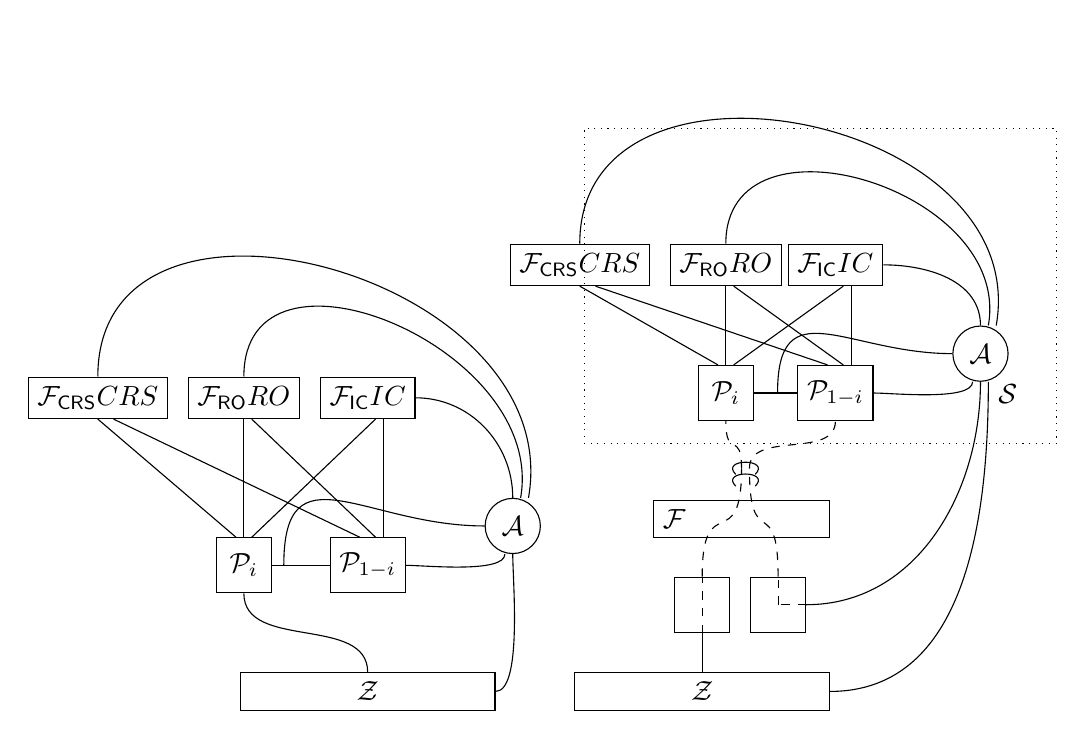
\begin{tikzpicture}[node distance=0.25cm]
  %left picture
  \node[rectangle,draw,fill=none] (fro) {\Fro};
  \node[rectangle,draw,fill=none] (fic) [right=of fro] {\Fic};  
  \node[rectangle,draw,fill=none] (fcrs) [left=of fro] {\Fcrs};
  \node[rectangle,draw,fill=none,minimum size=0.7cm] (pi) [below=1.5cm of fro] {$\aparty$};
  \node[rectangle,draw,fill=none,minimum size=0.7cm] (pj) [below=1.5cm of fic] {$\otherparty$};
  \node[circle,draw,fill=none] (adv) [right=1cm of pj,yshift=0.5cm] {\AdvA};
  \node[rectangle,draw,fill=none,text width=3cm,text centered] (env) [below=1cm of pj] {\Env};
  % from the parties to the helping functionalities
  \draw[-] (fro.south) edge (pi.north);
  \draw[-] ([xshift=0.1cm] fic.south) edge ([xshift=0.1cm] pi.north);
  \draw[-] ([xshift=0.1cm] fro.south) edge ([xshift=0.1cm] pj.north);
  \draw[-] ([xshift=0.2cm] fic.south) edge ([xshift=0.2cm] pj.north);
  \draw[-] ([xshift=0.2cm] fcrs.south) edge ([xshift=-0.1cm] pj.north);
  \draw[-] (fcrs.south) edge ([xshift=-0.1cm] pi.north);
  % between parties
  \draw[-] (pi.east) edge (pj.west);
  % from environment to (honest) parties
  \draw[-] (env.north) edge[out=90,in=270] (pi.south);
  % from environment to adversary
  \draw (env.east) edge[out=0,in=270,looseness=0.5] (adv.south);
  % from adversary to corrupted parties
  \draw[-] ([xshift=-0.1cm] adv.south) edge[out=270,in=0,looseness=0.5] (pj.east);
  % the adversary controlling the channel
  \draw[-] ([xshift=0.15cm] pi.east) edge[out=90,in=180,looseness=1.5] (adv.west);
  % from adversary to helping functionalities
  \draw (adv.north) edge[out=90,in=0] (fic.east);
  \draw ([xshift=0.1cm] adv.north) edge[out=80,in=90,looseness=1.3] (fro.north);
  \draw ([xshift=0.2cm] adv.north) edge[out=80,in=90,looseness=1.3] (fcrs.north);
%   \coordinate (dotsleft) at ($(pi.west)$);
%     \draw [thick,dotted,-] ($(dotsleft)+(-0.2cm,0cm)$) -- ($(dotsleft)+(-0.5cm,0cm)$);
 
  %right picture
  \node[rectangle,draw,fill=none,text width=3cm,text centered] (env1) [right=1cm of env] {\Env};
  \node[rectangle,draw,fill=none,minimum size=0.7cm] (pi1) [above=0.5cm of env1] {};
  \node[rectangle,draw,fill=none,minimum size=0.7cm] (pj1) [right=of pi1] {};
  \node[rectangle,draw,fill=none,text width=2cm] (f) [above=1.7cm of env1,xshift=0.5cm] {\Func};
  
  %simulator's box
  \node[rectangle,draw,fill=none,dotted,minimum width=6cm,minimum height=4cm,
   text width=5cm,text height=3cm,align=right] (sbox) [above=2.9cm of env1,xshift=1.5cm] {\Sim};
  \node[rectangle,draw,fill=none,minimum size=0.7cm] (spi) [above=1cm of f,xshift=-0.2cm] {$\aparty$};
  \node[rectangle,draw,fill=none,minimum size=0.7cm] (spj) [right=of spi,xshift=0.3cm] {$\otherparty$};
  \node[rectangle,draw,fill=none] (sfro) [above=1cm of spi]{\Fro};
  \node[rectangle,draw,fill=none] (sfic) [above=1cm of spj] {\Fic};
  \node[rectangle,draw,fill=none] (sfcrs) [left=of sfro] {\Fcrs};
  \node[circle,draw,fill=none] (sadv) [right=1cm of spj,yshift=0.5cm] {\AdvA};
  % from the parties to the helping functionalities
  \draw[-] (sfro.south) edge (spi.north);
  \draw[-] ([xshift=0.1cm] sfic.south) edge ([xshift=0.1cm] spi.north);
  \draw[-] ([xshift=0.1cm] sfro.south) edge ([xshift=0.1cm] spj.north);
  \draw[-] ([xshift=0.2cm] sfic.south) edge ([xshift=0.2cm] spj.north);
  \draw[-] ([xshift=0.2cm] sfcrs.south) edge ([xshift=-0.1cm] spj.north);
  \draw[-] (sfcrs.south) edge ([xshift=-0.1cm] spi.north);
  % between parties
  \draw[-] (spi.east) edge (spj.west);
  % from environment to adversary
  \draw[-] ([xshift=0.1cm]sadv.south) edge[out=270,in=0] (env1.east);
  % from adversary to corrupted parties
  \draw[-] ([xshift=-0.1cm] sadv.south) edge[out=270,in=0,looseness=0.5] (spj.east);
  % the adversary controlling the channel
  \draw[-] ([xshift=0.3cm] spi.east) edge[out=90,in=180,looseness=1.5] (sadv.west);
  % from adversary to helping functionalities
  \draw (sadv.north) edge[out=90,in=0] (sfic.east);
  \draw ([xshift=0.1cm] sadv.north) edge[out=80,in=90,looseness=1.3] (sfro.north);
  \draw ([xshift=0.2cm] sadv.north) edge[out=80,in=90,looseness=1.3] (sfcrs.north);

  % wires outside the simulator
  \draw[-] (sadv.south) edge[out=270,in=0] (pj1.east); %adversary controlling right party
  \draw[-] (pj1.east) edge[dashed] (pj1.center); %wires inside right party
  \draw[-] (pj1.center) edge[dashed] (pj1.north);
  \node (mergepoint) [above=0.4cm of f] {}; %dummy node for mergepoint
  \draw[-] (pj1.north) edge[dashed,out=90,in=270,looseness=2] ([xshift=0.1cm]mergepoint.south); % the two merged wires, lower part
  \draw[-] (pi1.north) edge[dashed,out=90,in=270,looseness=2] (mergepoint.south);
  \draw[-] ([xshift=0.1cm]mergepoint.south) edge[dashed,out=90,in=270,looseness=1] (spj.south); %upper part
  \draw[-] (mergepoint.south) edge[dashed,out=90,in=270,looseness=2] (spi.south);
  \draw[-] ([yshift=-0.2cm,xshift=0.05cm]mergepoint.east) edge[looseness=3] ([yshift=-0.2cm,xshift=0.05cm]mergepoint.west); % the curve tying the wires together
  \draw[-] ([yshift=-0.35cm,xshift=0.05cm]mergepoint.east) edge[looseness=3] ([yshift=-0.35cm,xshift=0.05cm]mergepoint.west);
  \draw[-] (env1.north) edge (pi1.south); % from Z to left party
  \draw[-] (pi1.south) edge[dashed] (pi1.north); %inside left party
\end{tikzpicture}
 \caption{Transition from game~\printgame{iPAKEreal} (left) to game~\printgame{iPAKElayout} (right), showing a setting where $\otherparty$ is corrupted.}
\end{figure}
  
  
% **************************************************************
%                                                              *
%  Layout
%                                                              *
% **************************************************************
\game{iPAKElayout} 
\textbf{Modeling the ideal layout.}
We first regroup and create new machines, similar to Game 1 in the proof of Theorem~\ref{theorem:fake2}. The new machine \Sim executes the code of the CRS, RO and IC functionalities as depicted in Figures~\ref{functionality:CRS}, \ref{functionality:RO}, and~\ref{functionality:IC}.

% **************************************************************
%                                                              *
%  Birthday
%                                                              *
% **************************************************************
\game{iPAKEbirthday}
\textbf{Simulating the ideal functionalities.}
We modify simulation of \Fro and \Fic as follows. We let \Sim implement Figure~\ref{functionality:IC} by maintaining a list \ListIC with entries of the form $(k,m,\alpha,\Encrypt|\Decrypt,c)$. \Sim handles encryption and decryption queries as follows:
\begin{itemize}
 \item Upon receiving $(\sid,\Encrypt,\key,m)$ (for shortness of notation, we will also write $\Encrypt_\key(m)$ for this query), if $\key\notin \F_\alphabetsize$ or $m\notin \G$ then abort. Else, if there is an entry $(\key,m,*,*,c)$ in \ListIC, \Sim replies with $(\sid,c)$. Else, \Sim chooses $c\getsr \G\setminus\{1\}$. If there already is a record $(*,*,*,*,*,c)$ in \ListIC, \Sim aborts. Else, \Sim adds $(\key,m,\bot,\Encrypt,c)$ to \ListIC and replies with $(\sid,c)$.
 \item Upon receiving $(\sid,\Decrypt,\key,c)$ (or $\Decrypt_\key(c)$, for short), if $\key\notin \F_\alphabetsize$ or $c\notin \G$ then abort. Else, if there is an entry $(\key,m,*,*,c)$ in \ListIC, \Sim replies with $(\sid,m)$. Else, \Sim chooses $\alpha\gets \F_q^*$. If there already is a record $(*,*,g^\alpha,*,*,*)$ in \ListIC, \Sim aborts. Else, \Sim adds $(\key,g^\alpha,\alpha,\Decrypt,c)$ to \ListIC and replies with $(\sid,g^\alpha)$.
\end{itemize} 
Similarly, let \ListRO denote the list that \Sim maintains upon implementing Figure~\ref{functionality:RO}, containing entries of the form $(m,h)$. We let \Sim handle queries to \Fro as follows:
\begin{itemize}
\item Upon receiving $H(m)$, if $m\notin \bits^*\times\bits^*\times\G^3$, then abort.
Else, if there is an entry $(m,h)$ in \ListRO, \Sim replies with $(\sid,h)$. Else, \Sim chooses $h\getsr \bits^k$.
If there already is a record $(*,*,h)$ in \ListRO, \Sim aborts. Else, \Sim adds $(m,h)$ to \ListRO and replies with $(\sid,h)$.
\end{itemize}
%NOTE: H is globally collision resistant since the check does not depend on \sid.

These modifications later allow \Sim to extract unique inputs from values obtained from the two functionalities. Especially, note that \ListIC will never contain $(*,\akey,*,*,\Encrypt,c)$, $(*,\otherkey,*,*,\Encrypt,c)$ with $\akey\neq \otherkey$. The entry $\alpha$ serves \Sim as a trapdoor for solving discrete-log type problems.

Since $q$ is greater than $2^\SEC$, if the oracles are only queried a polynomial number of times, the birthday problem states that game~\previousgame and game~\thisgame are indistinguishable with probability overwhelming in $\SEC$.

% **************************************************************
%                                                              *
%  build layout of F
%                                                              *
% **************************************************************
\game{iPAKEbuildF} 
\textbf{Building $\FiPAKE$.} In this game, we start modeling $\FliPAKE$.
First, we let \Func maintain two initially empty lists: $\Lpw$, a list of tuples of the form $(\aparty,\apw)$ and $\Ll$, a list of tuples of the form $(\aparty,\ell)$. Upon receiving a query $(\NewSession,\sid,\apw,\ell)$ from (dummy) party $\aparty$, if this is the first \NewSession query, or if this is the second \NewSession query and there is a record~$(\otherparty,\otherpw,\ell')$, then \Func records~$(\aparty,\apw)$ in $\Lpw$ and marks this record  as \web{fresh}.
If $\Ll$ does not contain any record $(\aparty,\cdot)$ so far, \Func also records $(\aparty,\ell)$ in $\Ll$. Then, \Func relays the query $(\NewSession,\sid,\apw,\ell)$ to \Sim. Now that \Func knows about \passwords and labels, we can add a \TestPwd interface to \Func as described in Figure~\ref{fig:func-iPAKE}.
We let \Sim parse outputs $(\sid,\ell',\akey)$ towards \Func to be of the form $(\NewKey,\sid,\aparty,\ell',\akey)$ by adding the \NewKey tag and the name of the party who produced the output.
\expl{The labels will be in the \NewKey queries only for the following hybrids, and they are removed in a later game when \Func is fully build.}
Additionally, we let \Func translate this back to $(\sid,\ell',\akey)$ and send it to \Env via the dummy party $\aparty$, marking the corresponding record as \web{completed}.

None of these modifications changes the output towards \Env compared to the previous game~\previousgame. 
\expl{Two possibilities now: 1) remove label from NewKeys step by step or 2) remove then now altogether. In any case, the proof has to show: if not attacked, the labels are not modified. this means we cannot remove them now, since labels cannot be overwritten in \Func yet (no testpwd by sim so far) but they can be in the real execution, so there the label might change! thus 2) is not an option and we do 1).}

% **************************************************************
%                                                              *
%  random session key for interrupted session
%                                                              *
% **************************************************************
\game{iPAKEinterrupted}
\textbf{\Func generates a random session key for an honest, interrupted session.}
Upon receiving a query $(\NewKey,\sid,\aparty,\akey)$ from \Sim, if $\aparty$ is not corrupted and there is a record of the form~$(\aparty,\apw)$ that is marked as \web{interrupted}, and this is the first \NewKey query for~$\aparty$, we let \Func choose a random session key $\key^*$ of length $\SEC$. Additionally, \Func derives the label as follows: if there is a record $(\otherparty,\ell^*)$ in $\Ll$, extract $\ell^*$ from it; otherwise, set $\ell^*\gets\bot$. Then, \Func outputs $(\sid,\ell^*,\key^*)$ to $P$.

If there is no such interrupted record, \Func continues to relay $\akey$ and $\ell'$.
% \sophia[inline]{This is still exactly the idea functionality, right?}

Since the simulators described in game~\previousgame and game~\thisgame do not make use of the \TestPwd interface, none of the records of \Func are marked as \web{interrupted} and thus the output towards \Env is equally distributed in both games.

% **************************************************************
%                                                              *
%  Dictionnary attacks against \aparty (using m-i-t-m or corruption)
%                                                              *
% **************************************************************
\game{iPAKEdictPi}
\textbf{\Sim handles dictionary attacks against the client $\firstparty$ using the \TestPwd interface.}
\expl{We cannot define \Sim in a way that a private $H'$ is only used for interrupted session as in the ACCP08 proof, since \Sim does not know. If we do change it, $H'$ also is used for compromised, which is detectable  since \Env might know the exponent of the element $g^x_\Env$ from its \password guess. I.e., \Env can reproduce an honest parties input to \Fro if he guesses successfully. In the $\Pr[BAD]=negl$ Lemma, we thus take a different approach of letting the CDH attacker decide whether to use $H'$ or not (in fact, since no $H'$ output is affecting anything, we just send $\sk=\bot$ and let \Func replace that with a random key later).}
In this game, we will only change the simulation. First note that the client, the initiator of the protocol, is intended to send the first message, and we call him $\firstparty$. If both $\firstparty$ and $\secondparty$ are honest, $\firstparty$ obtained input and \Env advises \AdvA to substitute $(\sid,\ell',Y^*)$ with $(\sid,\ell_\Env,Y^*_\Env)$, or if $\secondparty$ is corrupted and produces $(\sid,\ell_\Env,Y^*_\Env)$ as first flow, then \Sim will proceed simulation of $\firstparty$ using $\ell_\Env$ and $Y^*_\Env$.
\expl{Note that this includes the attack where \Env *just* changes the label and keeps the rest (i.e.,$Y^*$ or $X^*$) as it was. This should result in a \TestPwd query, since you should not be able to substitute the label (authenticated information) without knowing the \password.}
In this situation, we modify \Sim as follows:
upon receiving $(\sid,\ell_\Env,Y^*_\Env)$, if there is an entry $(\pw_\Env||\hat\ell,*,*,\Encrypt,Y^*_\Env)$ for any $\hat\ell\in\mathcal{L}$ in \ListIC\footnote{This entry is unique due to simulation of \Fic as described in game~\printgame{iPAKEbirthday}.}, the simulator asks a \TestPwd query $(\TestPwd,\sid,\firstparty,\pw_\Env,\ell_\Env)$ to \Func. \Sim then proceeds the simulation using $\pw_\Env$ and $\ell_\Env$ instead of $\firstpw$ and $\ell'$\footnote{Note that, since \Func does not leak any information at this point, \Sim cannot depend on the outcome of a \TestPwd query.}. If there is no entry $(\pw_\Env||\hat\ell,*,*,\Encrypt,Y^*_\Env)$ in \ListIC, \Sim sends $(\TestPwd,\sid,\firstparty,\firstpw,\ell_\Env)$ to \Func\footnote{Letting \Sim guess a \password that he actually knows seems a little artificial. Indeed, the simulation in this case will be changed in game~\printgame{iPAKEpw_honestPi} when \Sim becomes oblivious of $\firstparty$'s \password.}.
%NOTE: this makes it complicated later, but it seems not to be very clean to just submit a random \password to \TestPwd.
%\pad{Maybe we could send a dummy \password at this point, instead of in game~\printgame{iPAKEpw_honestPi}}
%\julia[inline]{We could, but the whole layout of the proof is 1. switch to random session keys and 2. switch to simulated \passwords. So I'd rather change the \passwords later.}

Regarding the label, observe that \Sim's \NewKey query will contain $\ell_\Env$ which was contained in the output of the honest $\firstparty$ (cf. Figure~\ref{fig:UC-EKE2}). Since \TestPwd queries overwrite any existing labels, there will be an entry $(\secondparty,\ell_\Env)$ in $\Ll$ and thus, regarding the label, the output towards \Env does not change compared to the previous game. Regarding the session key, we have to analyze different cases depending on whether $Y^*_\Env$ was generated using \Fic or not. However, observe that the only changes of session keys between this and the previous game occur whenever a \TestPwd query of \Sim causes a record to be marked as \web{interrupted}.

\begin{itemize}
 \item There is an entry $(\pw_\Env||\hat\ell,*,*,\Encrypt,Y^*_\Env)$ in \ListIC: if $\pw_\Env=\firstpw$, the record is marked \web{compromised} and the session key is not changed by \Func. If $\pw_\Env\neq\firstpw$, on the other hand, the record is marked \web{interrupted} and \Func hands out a random session key, as opposed to game~\previousgame. 
	 %Furthermore, the rest of the transcript (i.e., $Y^*$) is produced using $\pw_\Env$ instead of $\otherpw$.
	 However, since the session key is distributed as before, \Env can only detect this by reproducing $\firstparty$'s input $(\sid,X^*,Y^*_\Env,\CDH(\Decrypt_{\firstpw||\ell}(X^*)$, $\Decrypt_{\firstpw||\ell_\Env}(Y^*_\Env))$ to \Fro. 
 %check effect of generating Y with a different \password. Analyze w.r.t. \ListIC entries. Should be no problem since Y is the only leakage of the randomness used by \otherparty in an interrupted session. Checked.
 \expl{It might seem stupid of \Env to add a different label, but it still can do this. However, if the \password is not correct, the resulting key is random anyway. If it is correct, the simulated session key will get through, which will be random due to \Fro/\Fic when there is no record with key $\apw||\ell_\Env$ yet. So no problem here.}
Lemma~\ref{lemma:BAD1} (see below) shows indistinguishability of game~\previousgame and game~\thisgame.
 \item There is no entry $(*,*,*,\Encrypt,Y^*_\Env)$ in \ListIC: since the \TestPwd query will result in a compromised record, the modified simulation has no impact on the output towards \Env in this case.
%NOTE: this is easy now but will be complicated later when we substitute \pw' by \pw_\Sim. We will have to analyze w.r.t. entries (...\Decrypt...) and might make use of \alpha in these entries.
\end{itemize}

The following lemma bounds the probability that an unsuccessful dictionary attack leads to a non-random looking session key. Since in this case the labels do not play any role (the encryption keys of the form $\password||label$ will not match regardless of the labels), we ignore them for the sake of simplicity.
\begin{lemma}\label{lemma:BAD1}
If \CDH holds in $\G$, then $\forall \firstpw,Y^*_\Env\gets\Env$, where $Y^*_\Env$ is a ciphertext generated through \Fic with some key $\pw_\Env\neq\firstpw$, $\firstpw\in\F_\alphabetsize$, it holds that 
 \[
  \Pr_{\thisgame}[\CDH(\Decrypt_{\firstpw}(X^*),\Decrypt_{\firstpw}(Y^*_\Env))\gets\Env(X^*)]=negl(\SEC).
 \]
\end{lemma}
\begin{proof}
 We create an attacker \BCDH given a \CDH instance $(g,A = g^a,B = g^b)$.
\BCDH runs \Env simulating game~\thisgame as follows:
\BCDH internally runs all of the participating machines, i.e. \Sim, \Func and the dummy parties as in game~\thisgame, but with some modifications.
First, \BCDH computes $X^*\gets\Encrypt_{\firstpw}(A)$ and updates \ListIC accordingly, aborting if there already was an entry $(\firstpw,A,*,\Encrypt,*)$.
Upon receiving a query $\Decrypt_{\firstpw}(Y^*_\Env)$, \BCDH again aborts if there already is an entry $(\firstpw,*,*,\Encrypt,Y^*_\Env)$.
Otherwise, it draws $\beta\getsr\F_q$ and sets the answer to this query to be $B g^\beta$.
This can happen multiple times (for different $Y^*_\Env$), and \BCDH keeps track of the pairs $(\beta,Y^*_\Env)$ in a list \ListCDH.
The last modification concerns the part of the simulator's code of game~\thisgame where a value $Z\gets\Decrypt_{\firstpw}(Y^*)^a$ needs to be computed, but note that \BCDH does not know $a$.
Instead, \BCDH just sets $Z\gets\bot$.
%Observe that in the honest case $Z'$ is computable by \Sim since $\otherparty$ uses $Y^*$ where \Sim knows $y$.

Finally, \BCDH picks a random entry from \ListRO asked by the environment, parses it as $((\firstpw,X^*,Y^*_\Env,Z),h)$, looks for an entry $(\beta,Y^*_\Env)$ in \ListCDH and outputs $Z/(g^a)^\beta$ as a \CDH solution.

First, note that if \BCDH does not abort, it perfectly emulates \Env's view in game~\thisgame, since $A,B g^{\beta}$ are random in $\G$ and the record for $\firstparty$ will be interrupted, which means that \Func will output a random session key for $\firstparty$, overwriting $\bot$. Second, \BCDH only has to abort if there is a collision upon choosing random values from $\G$.

Assume that \Env outputs $\CDH(\Decrypt_{\firstpw}(X^*),\Decrypt_{\firstpw}(Y^*_\Env))$ with non-negligible probability. This is only possible if \Env asked  both corresponding decryption queries. Existence of $(\pw_\Env,*,*,\Encrypt,Y^*_\Env)$ with $\pw_\Env\neq\firstpw$ in \ListIC ensures that the answer to $\Decrypt_{\firstpw}(Y^*_\Env)$ can be chosen by \BCDH as described above. Thus, \BCDH finds a correct \CDH solution with non-negligible probability $1/q_\Env$, where $q_\Env$ is the number of hash queries issued by \Env.
\end{proof}
 
% **************************************************************
%                                                              *
%  Dictionnary attack against \otherparty (using m-i-t-m or corruption)
%                                                              *
% **************************************************************
\game{iPAKEdictPj}
\textbf{\Sim handles dictionary attacks against the server $\secondparty$ using the \TestPwd interface.}
Again, in this game we only change the simulation. Analogously to game~\previousgame, we let \Sim use the \TestPwd interface upon receiving adversarially generated $X^*_\Env,\ell_\Env$ upon simulating $\secondparty$. Observe that the only difference is due to the order of flows: if \Sim extracts an incorrect \password, he produces $Y^*$ using this wrong \password. However, $Y^*$ will be distributed as before and again, \Env can only detect the change by reproducing $\secondparty$'s input to \Fro, namely $(\sid,X^*_\Env,Y^*,\CDH(\Decrypt_{\secondpw||\ell_\Env}(X^*_\Env)$, $\Decrypt_{\secondpw||\ell'}(Y^*))$.

Using an analogous argument to Lemma~\ref{lemma:BAD1}, indistinguishability from game~\previousgame follows from the hardness of \CDH in $\G$.

% **************************************************************
%                                                              *
%  F aligns session keys
%                                                              *
% **************************************************************
\game{iPAKEalignSK} 
\textbf{\Func aligns session keys.}
Upon receiving a query $(\NewKey,\sid,\aparty,\ell',\akey)$ from \Sim for a session, if this query is \emph{due} then output~$(\sid,\ell^*,\key^*)$ to~$\aparty$ where $\key^*$ is the session key that was formerly sent to the other party and the label $\ell^*$ is derived as usual: if there is a record $(\otherparty,\ell^*)$ in $\Ll$, extract $\ell^*$ from it; otherwise, set $\ell^*\gets\bot$. 
% \expl{We have to add ``where none of the players is corrupted'' here although it is not written like this in $\FliPAKE$. The reason is that in case of $\otherparty$ corrupted with matching key, $\FliPAKE$ lets the adversary determine the key and this triggers *before* the alignment bullet can trigger. Since during the game hops we only modify \Func to *not* relay keys in specific cases, we have to exclude everything manually. Note that ``compromised'' and ``$\aparty$ corrupted'' is automatically excluded for a due record. Update: deprecated since we now have due=honest session.}
 
We now analyze distinguishability of this game from game~\previousgame.
% NOTE: the following was removed upon modifying iPAKE so that a corrupted \otherparty with a matching \password receives sk from the adversary. 
% First, we consider the case where the other party is corrupted. Since in this case the simulation ensures that the record $(P,*,\pw)$ is either compromised or interrupted (cf. description of the simulator in games~\printgame{iPAKEdictPi} and~\printgame{iPAKEdictPj}), the modifications have no effect since they only concern fresh records. 
If \Env tampered with the transcript, any player that received a modified message will not have a fresh record anymore (cf. simulation described in games~\printgame{iPAKEdictPi} and~\printgame{iPAKEdictPj}) and the output of this player towards \Env is not changed in this game.
On the other hand, if \Env does not advise \AdvA to tamper with any message, \Func did not overwrite any labels and thus $\ell^*=\ell'$. Additionally, perfect correctness of the EKE2 protocol ensures that, in case of a due record, $\akey=\key^*$.

Note that \Func still differs from the functionality $\FliPAKE$ described in Figure~\ref{fig:func-iPAKE} in some aspects. First, it does not output randomly generated session keys towards \Env for honest sessions. Furthermore, it reports all \passwords to \Sim. We will take care of these remaining differences in the next games.



% **************************************************************
%                                                              *
%  F generates random sk if other party is corrupted with non-matching pw
%                                                              *
% **************************************************************
\game{iPAKEdummy}
\textbf{In some cases, \Func generates a random session key when the other party is corrupted.}
Upon receiving a \NewKey query $(\NewKey,\sid,\aparty,\ell',\akey)$ from \Sim, if there is a fresh record of the form~$(\aparty,\apw)$ in $\Lpw$, and this is the first \NewKey query for~$\aparty$, $\aparty$ is honest and $\otherparty$ corrupted and there is a record $(\otherparty,\otherpw)$ in $\Lpw$ with $\apw\neq\otherpw$, we let \Func pick a new random key~$\key^*$ of length~$\SEC$ and send~$(\sid,\ell^*,\key^*)$ to~$\aparty$, where $\ell^*$, as usual, is taken from the list $\Ll$ or set to be $\bot$. 

The simulation ensures that the record $(\aparty,\apw)$ is either compromised or interrupted (cf. description of the simulator in games~\printgame{iPAKEdictPi} and~\printgame{iPAKEdictPj}). Thus, the modification has no effect since it only concerns fresh records. 
\expl{This game handles the only case where a session with a corrupted player might get a random session key from \Func. The argument will get more complicated when there are adaptive corruptions.}

% **************************************************************
%                                                              *
%  F generates random sk for honest session
%                                                              *
% **************************************************************
\game{iPAKErandomSK}
\textbf{\Func generates a random session key for an honest session.}
Upon receiving a \NewKey query $(\NewKey,\sid,\aparty,\ell',\akey)$ from \Sim, if there is a fresh record of the form~$(\aparty,\apw)$ in $\Lpw$, and this is the first \NewKey query for~$\aparty$, both parties are honest and the \NewKey query is not \emph{due}, we let \Func pick a new random key~$\key^*$ of length~$k$ and send~$(\sid,\ell^*,\key^*)$ to~$\aparty$, where $\ell^*$, as usual, is taken from the list $\Ll$ or set to be $\bot$.  

In other words, \Func now generates a random session key upon a first \NewKey query for an honest party $\aparty$ with fresh record $(\aparty,\apw)$ where the other party is also honest, if (at least) one of the following events happens:
\begin{enumerate}
 \item There is a record $(\otherparty,\otherpw)$ in $\Lpw$ with $\apw\neq\otherpw$;
 \item No output was sent to the other party yet;
 \item If there was output to the other party, the record $(\otherparty,\otherpw)$ in $\Lpw$ was not fresh and thus interrupted or compromised at that time
\end{enumerate} 
 In all of these cases, \Sim chose a fresh $\akey$ following a uniform distribution and $\ell'$ was contained in the \NewSession query of $\aparty$'s partner, thus $\ell'=\ell^*$. Regarding the session key, \Env can only notice a difference if it reproduces $\akey$ by computing $\aparty$'s input $(\sid,X^\ast,Y^\ast,\CDH(\Decrypt_{\apw||\ell}(X^*),\Decrypt_{\apw||\ell'}(Y^*))$ to \Fro and sending it to \Fro via the adversary \AdvA.
 
The following lemma bounds the probability that a session key of an unattacked session does not look random.
\begin{lemma}\label{lemma:BAD2} 
 If \CDH holds in $\G$, then $\forall \pw,\ell,\ell'\gets\Env$ with $\pw\in\F_\alphabetsize$ and $\ell,\ell'\in\mathcal{L}$ it holds that 
 \[
  \Pr_{\thisgame}[\CDH(\Decrypt_{\pw||\ell}(X^*),\Decrypt_{\pw||\ell'}(Y^*))\gets\Env(X^*,Y^*)]=negl(\SEC).
 \] 
\end{lemma}
\begin{proof}
 We only sketch the proof since it is similar to the proof of Lemma~\ref{lemma:BAD1}. Namely, the strategy of embedding (randomized versions of) a \CDH challenge into the simulation of game~\printgame{iPAKErandomSK} is done by just encrypting both \CDH challenge elements to obtain $X^*$ and $Y^*$. For the final argument, note that $\bot$ is not seen by \Env since it is either replaced using a random session key or a previously computed key. 
\end{proof}
It follows that game~\previousgame and game~\thisgame are indistinguishable.

% **************************************************************
%                                                              *
%  remove labels from \NewKey
%                                                              *
% **************************************************************
\game{iPAKElabels}
\textbf{\Func always takes all labels from the list $\Ll$.}
We modify \Func as follows: if \Func outputs $(\sid,\ell',\akey)$ towards $\aparty$ where $\ell',\akey$ are taken from a query $(\NewKey,\sid,\aparty,\ell',\akey)$ from \Sim, \Func extracts $\ell^*$ from a record $(\otherparty,\ell^*)$ in $\Ll$ or sets $\ell^*\gets\bot$ if such a record does not exist. \Func then outputs $(\sid,\ell^*,\akey)$ towards $\aparty$. We additionally modify \Sim to remove the labels from the \NewKey queries altogether.

First observe that we can remove the labels from the \NewKey queries because, in this and the past games, we ensured that \Func now does not access this label anymore. However, we still have to argue indistinguishability of the current and the previous game. The cases where $\akey$ of \Sim is relayed by \Func towards $\aparty$ are the following:
\julia[inline]{The label is taken from the label list by \Func in any case, not only in case of a relayed session key. Don't we have to argue indistinguishability of the due/align and other/random case as well?}
\begin{itemize}
 \item $\aparty$ has a compromised record
 \item $\aparty$ is corrupted
 \item $\aparty$ has a fresh record, its partner is corrupted and has a record with a matching \password
\end{itemize}
In the first case, we have that $\ell'=\ell^*$ since the label $\ell'$ outputted by $\aparty$ was also contained in a \TestPwd query by \Sim and overwrote any existing label send by $\aparty$'s partner. For the second case, observe that since we restrict to static corruption, corrupted players will not have records in $\Lpw$ and thus this case will never happen. 
\expl{This argument for corrupted players getting \NewKey queries needs to be more sophisticated when we consider adaptive corruption!}
In the third case, corruption of the partner ensures that \Sim issued a \TestPwd query which overwrote any existing label with $\ell'$, so $\ell'=\ell^*$ as well.

Observe that now \Func acts like $\FliPAKE$ regarding the output of session keys and labels. The only remaining difference is that the \NewSession queries still contain the \passwords of the parties. In the next games, we will make the simulation independent of these \passwords.

% **************************************************************
%                                                              *
%  remove \password of corrupted party
%                                                              *
% **************************************************************
% %wlog, we say that a corrupted party does not receive a NewSession query from Z. Thus, this part is removed.
% \game{iPAKEpw_Picorrupted}
% \textbf{Simulate without $\pw$ for corrupted parties.}
% In case of receiving a $(\NewSession,\sid,P,*,\pw)$ from a corrupted $P$, we modify \Func by forwarding only $(\NewSession,\sid,P,*)$ to \Sim.
% However, in the byzantine corruption model \cite[Section 6.1]{FOCS:Canetti01}, as $P$ is corrupted, the original \NewSession query was seen by \Sim \emph{before} it was seen by \Func, and thus \Sim still knows $\pw$ and can proceed with the exact same simulation as in game~\previousgame.
% 
% Obviously, the output towards \Env is not affected by this modification and thus game~\previousgame and game~\thisgame are perfectly indistinguishable for \Env.

% **************************************************************
%                                                              *
%  remove \password of honest Pj
%                                                              *
% **************************************************************
\game{iPAKEpw_honestPj}
\textbf{Simulate without $\secondpw$ if server $\secondparty$ is honest.}
In case of receiving a $(\NewSession,\sid,\secondpw,\ell')$ from an honest $\secondparty$ playing the role of a server, we modify \Func by forwarding only $(\NewSession,\sid,\secondparty,\ell')$ to \Sim. We now have to modify \Sim to proceed simulation without knowing $\secondpw$.
Upon receiving $(\NewSession,\sid,\secondparty,\ell')$ from \Func for an honest $\secondparty$, we let \Sim draw uniformly at random a ``dummy'' \password $\pw_\Sim$ and proceed the simulation of $\secondparty$ using $\pw_\Sim$ as a \password.

We first note that, if at any time \Sim sends a \NewKey query to \Func containing a session key $\secondkey$ for $\secondparty$, this session key is only seen by \Env if $\secondparty$'s record is compromised. Otherwise, we thus only have to argue indistinguishability of the transcripts of game~\previousgame and game~\thisgame. 

\begin{itemize}
 \item \Env sends $\ell_\Env,X^*_\Env$, there is a record $(\pw_\Env||\hat\ell,X,*,\Encrypt,X^*)$ in \ListIC for some $\hat\ell\in\mathcal{L}$ and $\pw_\Env=\secondpw$: since \Sim will issue a \TestPwd query that will result in a compromised record (cf. simulation described in game~\printgame{iPAKEdictPj}), nothing is changed since $\pw_\Sim$ was never used, and $Y^*$ is generated using the correct \password $\pw_\Env$.
 \item \Env sends $\ell_\Env,X^*_\Env$ , there is a record $(\pw_\Env||\hat\ell,X,*,\Encrypt,X^*)$ in \ListIC for some $\hat\ell\in\mathcal{L}$ and $\pw_\Env\neq\secondpw$: since $\secondparty$ will receive a random session key from \Func in this case (the record will be marked \web{interrupted}), we only have to argue indistinguishability of $Y^*$ generated with $\pw_\Env||\ell'$ instead of $\secondpw||\ell'$. Simulation of $\Fic$ ensures that $Y^*$ is distributed uniformly random as before. Observe that here it is crucial that even for a corrupted session, an interrupted record lets the functionality hand out a random session key, since \Sim has no means to decide whether it has to output a session key for $\secondparty$ that matches the session key that \Env can compute on behalf of $\firstparty$ from the message $(\ell',Y^*)$.
 \expl{Reason for changing the functionality regarding corrupted session: assume \Env mounts a dictionary attack by corrupting one player. In case of a \password match, \Sim has to make sure that the session key outputted by the honest party and the one that \Env can compute from the honest party's message match. In case of a wrong \password, \Sim has to make sure that they both look random. Now note that \Sim has no means to get information from \FliPAKE. To ensure matching session keys, \Sim has to proceed the honest party's simulation with the extracted \password. Now if the functionality always relays the session key computed by \Sim to \Env, this would always result in matching keys, no matter if the extracted \password matches the honest party's \password or not. \Sim needs help from the functionality, which has more information in this case and rescues \Sim by handing out a random session key in case of an unsuccessul dictionary attempt in a corrupted session.}
 \item \Env sends $\ell_\Env,X^*_\Env$ and no $\Encrypt$ record: the simulation described in game~\printgame{iPAKEdictPj}~tells \Sim to issue a \TestPwd query, but now using $\pw_\Sim$ instead of $\secondpw$. If, coincidentally, $\secondpw=\pw_\Sim$, nothing changes. On the other hand, if $\secondpw\neq\pw_\Sim$, $\secondparty$ obtains a random session key from \Func as opposed to the game before and $Y^*$ is created using $\pw_\Sim||\ell'$ instead of $\secondpw||\ell'$. This can only be detected if \Env reproduces $\secondparty$'s input to $\Fro$ from game~\previousgame, which happens only with negligible probability according to Lemma~\ref{lemma:BAD3} (see below). 
%  before: Y* with pw', session key with pw'
%  now: Y* with pw_j, random session key 
 \item both parties honest and no injections: $\secondparty$ will obtain a uniformly random session key from \Func in this case, and thus the only difference is that $Y^*$ was created using $\pw_\Sim||\ell'$ instead of $\secondpw||\ell'$. Again, this is indistinguishable since $Y^*$ is distributed exactly as before.
\end{itemize}

The following lemma bounds the probability that an injected $X^*$ that was not obtained using encryption leads to a non-random looking session key.
\begin{lemma}\label{lemma:BAD3}
 If \CDH holds in $\G$, then $\forall \secondpw,\ell',\ell_\Env,X^*_\Env\gets\Env$, where $X^*_\Env$ was not generated using \Fic, $\ell',\ell_\Env\in\mathcal{L}$ and $\secondpw\in\F_\alphabetsize$, it holds that 
 \[
  \Pr_{\thisgame}[\CDH(\Decrypt_{\secondpw||\ell_\Env}(X^*_\Env),\Decrypt_{\secondpw||\ell'}(Y^*))\gets\Env(Y^*)]=negl(\SEC).
 \] 
\end{lemma}
\begin{proof}
 Note that the only difference to Lemma~\ref{lemma:BAD1} is that this time, no record $(*,*,*,\Encrypt,X^*_\Env)$ exists so the fact that \BCDH is able to embed an element of its \CDH challenge into $\Decrypt_{\secondpw}(X^*_\Env)$ is even more obvious. The rest of the proof is analogously to Lemma~\ref{lemma:BAD1}.
\end{proof}

% **************************************************************
%                                                              *
%  remove \password of honest Pi
%                                                              *
% **************************************************************
\game{iPAKEpw_honestPi}
\textbf{Simulate without $\firstpw$ if client $\firstparty$ is honest.}
In a similar fashion, we now let \Func cut the \password from \NewSession queries to an honest $\firstparty$. We again have to modify \Sim to proceed simulation without knowing $\firstpw$. Upon receiving $(\NewSession,\sid,\firstparty,\ell)$ from \Func for an honest $\firstparty$, we let \Sim draw uniformly at random a ``dummy'' \password $\pw_\Sim$. \Sim proceeds the simulation of $\firstparty$ using $\pw_\Sim$ as a \password. 

Additionally, we further change \Sim in case of a dictionary attack against client $\firstparty$, i.e., upon receiving $\ell_\Env,Y^*_\Env$ from \Env. After submitting a \TestPwd query with an extracted $\pw_\Env$, we let \Sim now choose $x'\getsr\F_P$ and add $(\pw_\Env||\ell,g^{x'},x',\bot,X^*)$ to \ListIC and proceed the simulation of $\firstparty$ using $x'$ instead of $x$. 
% NOTE: \Sim needs to ``restart'' here by choosing x' and then setting \Decrypt_{\pw_\Env}(X^*):=g^x' to be able to compute a session key afterwards. This does not affect \Sim's output, it only lets \Sim fix it's random coins later on. This can not be detected if we only allow static corruption.

\begin{itemize}
 \item \Env sends $\ell_\Env,Y^*_\Env$, there is a record $(\pw_\Env||\hat\ell,Y,*,\Encrypt,Y^*)$ in \ListIC for some $\hat\ell\in\mathcal{L}$ and $\pw_\Env=\firstpw$: \Sim will issue a \TestPwd query that will result in a compromised record (cf. simulation described in game~\printgame{iPAKEdictPi}), resulting in a session key that is computed using $\pw_\Env$ instead of $\pw_\Sim$. Additionally, $X^*$ is generated using the incorrect \password $\pw_\Sim$. However, adjusting \ListIC as described above still allows \Sim to know the exponent of $\Decrypt_{\pw_\Env||\ell}(X^*)$ and continue the simulation, making it look like $\pw_\Env$ was used from the beginning. \Env's view is distributed exactly as before since $x',x$ are both uniformly random in $\F_P$.
 \item \Env sends $\ell_\Env,Y^*_\Env$ , there is a record $(\pw_\Env||\hat\ell,Y,*,\Encrypt,Y^*)$ in \ListIC for some $\hat\ell\in\mathcal{L}$ and $\pw_\Env\neq\firstpw$: since $\firstparty$ will receive a random session key from \Func in this case (the record will be interrupted), we only have to argue indistinguishability of $X^*$ generated with $\pw_\Sim|\ell$ instead of $\firstpw||\ell$. Simulation of $\Fic$ ensures that $Y^*$ is distributed uniformly random as before. Again, it is crucial here that \Func helps \Sim by randomizing the session key if needed.
 \item \Env sends $\ell_\Env,Y^*_\Env$ and no $\Encrypt$ record: the simulation described in game~\printgame{iPAKEdictPi}~tells \Sim to issue a \TestPwd query, but now using $\pw_\Sim||\ell$ instead of $\firstpw||\ell$. If, coincidentally, $\firstpw=\pw_\Sim$, nothing changes. On the other hand, if $\firstpw\neq\pw_\Sim$, $\firstparty$ obtains a random session key from \Func as opposed to the game before and $X^*$ was created using $\pw_\Sim||\ell$ instead of $\firstpw||\ell$. This can only be detected if \Env reproduces $\firstparty$'s input to $\Fro$ from game~\previousgame, which happens only with negligible probability using an argument very similar to Lemma~\ref{lemma:BAD3}. 
 \item both parties honest and no injections: $\firstparty$ will obtain a uniformly random session key from \Func in this case, and thus the only difference is that $X^*$ was created using $\pw_\Sim||\ell$ instead of $\firstpw||\ell$. Again, this is indistinguishable since $X^*$ is distributed exactly as before.
\end{itemize}
 
Observe that in game~\printgame{iPAKEpw_honestPi}, $\Func=\FliPAKE$\footnote{We note that we can, w.l.o.g, assume that there are no \NewSession queries from \Env to corrupted parties. Thus, it is enough to remove the \passwords from the \NewSession queries given as input from \Env to honest parties.}, and thus the theorem follows. The complete description of the simulator of game~\printgame{iPAKEpw_honestPi} interacting with $\FliPAKE$ and \Env is given in Figure~\ref{fig:sim-iPAKE}.
\end{games}

\begin{figure}[ht!]
  \centering
  \begin{fboxenv}
    \begin{minipage}{0.95\textwidth}
      The simulator \Sim, initialized with a security parameter \SEC, first runs a group generation algorithm using \SEC to obtain a cyclic group $\G$ with generator $g$ of order $q$ with $\log_2(q) \geq \SEC$. 
      Then, \Sim initializes the dummy adversary \AdvA.     
      \Sim then interacts with an ideal functionality $\FliPAKE$ and an environment \Env via the following queries:\\[-1.8em]
      \begin{itemize}
      \item
        \textbf{Upon receiving a query
        \mathversion{bold}$(\NewSession,\sid,\aparty,\ell)$ from $\FliPAKE$\mathversion{normal}:}
        \begin{itemize}
          \item initialize a party $\aparty$, connect it to \AdvA and proceed the UC protocol execution described in Figure~\ref{fig:UC-EKE2} using $\pw_{\Sim}\getsr\F_\alphabetsize$ as \password and \Sim's random coins. (Cf. games~\printgame{iPAKEreal},\printgame{iPAKEpw_honestPj}~and~\printgame{iPAKEpw_honestPi}.)
        \end{itemize}
      \item
        \textbf{Upon receiving a query
        \mathversion{bold}$(\sid,m)$ from any entity\mathversion{normal}:} (Cf. games~\printgame{iPAKElayout}~and~\printgame{iPAKEbirthday}.)\\
        If $m\notin \langle g\rangle^3$, then abort. Else:
        \begin{itemize}
          \item if there is an entry $(m,h)$ then reply with $(\sid,h)$. 
          \item else, choose $h\getsr\F_q$ and abort if there already is an entry $(*,*,h)$ in \ListRO. Else, reply with $(\sid,h)$.
        \end{itemize}
      \item
        \textbf{If an internally simulated party $\aparty$ produces an output 
        \mathversion{bold}$(\sid,\ell',\akey)$\mathversion{normal}:}\\
        Send $(\NewKey,\sid,\aparty,\akey)$ to $\FliPAKE$. (Cf. game~\printgame{iPAKElayout}.)
      \item
        \textbf{If \Env sends $(\sid,\ell_\Env,Z^*_\Env)$ to an honest party $\aparty$:}
        \begin{itemize}
         \item if $(\pw_\Env||\hat\ell,*,*,\Encrypt,Z^*_\Env)\in\ListIC$ for any $\hat\ell\in\mathcal{L}$, then send $(\TestPwd,\sid,\aparty,\pw_\Env,\ell_\Env)$ to $\FliPAKE$ and proceed the simulation of $\aparty$ with $\pw_\Env$. (Cf. games~\printgame{iPAKEdictPi}~and~\printgame{iPAKEdictPj}.)
         \item if $(*,*,*,\Encrypt,Z^*_\Env)\notin\ListIC$, then send $(\TestPwd,\sid,\aparty,\pw_\Sim,\ell_\Env)$ to $\FliPAKE$. (Cf. games~\printgame{iPAKEdictPi}~and~\printgame{iPAKEdictPj}.)
         \item if $\aparty$ was started with input $(\NewSession,\sid,\aparty,\ell)$, choose $x'\getsr\F_P$, add $(\pw_\Env||\ell,g^{x'},x',\bot,Z^*)$ to \ListIC and proceed as if $x'$ was the value drawn uniformly random from $\F_q$ at the beginning of the simulation of $\aparty$. (Cf. game~\printgame{iPAKEpw_honestPi}.)
        \end{itemize}

      \item
        \textbf{Upon receiving a query
        \mathversion{bold}$(\sid,\web{Encrypt},k,m)$ from any entity\mathversion{normal}:} (Cf. games~\printgame{iPAKElayout}~and~\printgame{iPAKEbirthday}.)\\
        If $k\notin\F_\alphabetsize$ or $m\notin\G$ then abort. Else:
        \begin{itemize}
          \item if there is an entry $(k,m,*,*,c)$ in \ListIC, reply with $(\sid,c)$
          \item else, choose $c\getsr\G\setminus\{1\}$. If there already is a record $(*,*,*,*,c)$ then abort. Else, add $(k,m,\bot,\Encrypt,c)$ to \ListIC and reply with $(\sid,c)$.
        \end{itemize}
      \item
        \textbf{Upon receiving a query
        \mathversion{bold}$(\sid,\web{Decrypt},k,c)$ from any entity\mathversion{normal}:} (Cf. games~\printgame{iPAKElayout}~and~\printgame{iPAKEbirthday}.)\\
        If $k\notin\F_\alphabetsize$ or $c\notin\G$ then abort. Else:
        \begin{itemize}
          \item if there is an entry $(k,m,*,*,c)$ in \ListIC, reply with $(\sid,m)$.
          \item else, choose $\alpha\getsr\F_\alphabetsize^*$. If there already is a record $(*,g^\alpha,*,*,*)$ then abort. Else, add $(k,g^\alpha,\alpha,\Decrypt,c)$ to \ListIC and reply with $(\sid,g^\alpha)$.
        \end{itemize}
      \item
        \textbf{Upon receiving a query
        \mathversion{bold}$(\sid,\web{crs})$ from any entity\mathversion{normal}: (Cf. game~\printgame{iPAKElayout}.)}
        \begin{itemize}
          \item reply with $(\sid,(g,q))$.
        \end{itemize}
      \end{itemize}
      Additionally, \Sim forwards all other instructions from \Env to \AdvA and reports all output of \AdvA towards \Env. Instructions of corrupting a player are only obeyed if they are received before the protocol started, i.e., before \Sim received any \NewSession query from $\FliPAKE$.
    \end{minipage}
  \end{fboxenv}
  \caption{The Simulator $\Sx$ for the EKE2 Protocol}\label{fig:sim-iPAKE}
\end{figure}


\section{Proof of Theorem~\ref{theorem:fake2}}
\label{sec:proofFake2}
% % !TEX root = ../main.tex


\begin{games}
% **************************************************************
%                                                              *
%  Real execution
%                                                              *
% **************************************************************
\game{real}
\textbf{The real protocol execution.}
This is the real execution of $\PfakeRSS$ where the environment \Env runs the protocol (cf. Figure \ref{fig:FAKERSS}) with parties $\firstparty$ and $\secondparty$, both having access to an ideal \liPAKE functionality $\FliPAKE$, and an adversary \AdvA that, w.l.o.g., can be assumed to be the dummy adversary as shown in \cite[section 4.4.1]{FOCS:Canetti01}.

% **************************************************************
%                                                              *
%  Layout
%                                                              *
% **************************************************************
\game{layout} 
\textbf{Modeling the ideal layout.}
We first make some purely conceptual changes that do not modify the input/output interfaces of \Env. We add one relay (also referred to as \emph{dummy party}) on each of the wires between \Env and a party. We also add one relay covering all the wires between the dummy parties and real parties and call it \Func (and let \Func relay messages according to the original wires). We group all the formerly existing instances except for \Env into one machine and call it \Sim. Note that this implies that \Sim executes the code of the \liPAKE functionality $\FliPAKE$. The differences are depicted in Figure~\ref{fig:g0g1layout} with $\Fot$ replaced by $\FliPAKE$.
%\julia[inline]{To David: the reference should actually go to the functionality in the appendix, where the code of \liPAKE is shown.}

% \begin{figure}[!ht]
%  \centering
% \begin{tikzpicture}[node distance=0.25cm]
%   %left picture
%   \node[rectangle,draw,fill=none] (flipake) {$\FliPAKE$};
%   \node[rectangle,draw,fill=none,minimum size=0.7cm] (pi) [below=1.5cm of flipake] {$\firstparty$};
%   \node[rectangle,draw,fill=none,minimum size=0.7cm] (pj) [right=1cm of pi] {$\secondparty$};
%   \node[circle,draw,fill=none] (adv) [right=1cm of pj,yshift=0.5cm] {\AdvA};
%   \node[rectangle,draw,fill=none,text width=3cm,text centered] (env) [below=1cm of pj] {\Env};
%   % from the parties to the helping functionalities
%   \draw[-] (flipake.south) edge (pi.north);
%   \draw[-] ([xshift=0.1cm] flipake.south) edge ([xshift=0.1cm] pj.north);
%   % between parties
%   \draw[-] (pi.east) edge (pj.west);
%   % from environment to (honest) parties
%   \draw[-] ([xshift=-0.5cm] env.north) edge[out=90,in=270] (pi.south);
%   \draw[-] ([xshift=0.5cm] env.north) edge[out=90,in=270] (pj.south);
%   % from environment to adversary
%   \draw (env.east) edge[out=0,in=270,looseness=0.5] (adv.south);
%   % the adversary controlling the channel
%   \draw[-] ([xshift=0.5cm] pi.east) edge[out=90,in=180,looseness=1.5] (adv.west);
%   % from adversary to helping functionalities
%   \draw ([xshift=0.1cm] adv.north) edge[out=80,in=0] (flipake.east);
% %   \coordinate (dotsleft) at ($(pi.west)$);
% %     \draw [thick,dotted,-] ($(dotsleft)+(-0.2cm,0cm)$) -- ($(dotsleft)+(-0.5cm,0cm)$);
%  
%   %right picture
%   \node[rectangle,draw,fill=none,text width=3cm,text centered] (env1) [right=1cm of env] {\Env};
%   \node[rectangle,draw,fill=none,minimum size=0.7cm] (dpi) [above=0.5cm of env1] {};
%   \node[rectangle,draw,fill=none,minimum size=0.7cm] (dpj) [right=of dpi] {};
%   \node[rectangle,draw,fill=none,text width=2cm] (f) [above=1.7cm of env1,xshift=0.5cm] {\Func};
%   
%   %simulator's box
%   \node[rectangle,draw,fill=none,densely dotted,minimum width=4.5cm,minimum height=3cm,
%    text width=4.5cm,text height=2.5cm,align=right] (sbox) [above=3cm of env1,xshift=1.5cm] {\Sim}; %dotted box
%   \node[rectangle,draw,fill=none,minimum size=0.7cm] (spi) [above=1.5cm of f,xshift=-0.2cm] {$\firstparty$};
%   \node[rectangle,draw,fill=none,minimum size=0.7cm] (spj) [right=of spi,xshift=0.3cm] {$\secondparty$};
%   \node[rectangle,draw,fill=none] (sfipake) [above=1cm of spi]{$\FliPAKE$}; 
%   \node[circle,draw,fill=none] (sadv) [right=1cm of spj,yshift=0.5cm] {\AdvA};
%   % wires from the parties to the helping functionalities
%   \draw[-] (sfipake.south) edge (spi.north);
%   \draw[-] ([xshift=0.1cm] sfipake.south) edge ([xshift=0.1cm] spj.north);
%   % wires between parties
%   \draw[-] (spi.east) edge (spj.west);
%   % wires from environment to adversary
%   \draw[-] ([xshift=0.1cm]sadv.south) edge[out=270,in=0] (env1.east);
%   % the adversary controlling the channel
%   \draw[-] ([xshift=0.3cm] spi.east) edge[out=90,in=180,looseness=1.5] (sadv.west);
%   % wires from adversary to helping functionalities
%   \draw ([xshift=0.1cm] sadv.north) edge[out=80,in=0] (sfipake.east);
%   
%   % wires outside the simulator
%   \draw[-] (dpj.south) edge[dashed] (dpj.north); %inside dummy party Pj
%   \draw[-] (dpi.south) edge[dashed] (dpi.north); %inside dummy party Pi
%   \node (mergepoint) [above=0.5cm of f] {}; %dummy node for mergepoint
%   \draw[-] (dpj.north) edge[dashed,out=90,in=270,looseness=2] ([xshift=0.1cm]mergepoint.south); % the two merged wires, lower part
%   \draw[-] (dpi.north) edge[dashed,out=90,in=270,looseness=2] (mergepoint.south);
%   \draw[-] ([xshift=0.1cm]mergepoint.south) edge[dashed,out=90,in=270,looseness=1.5] (spj.south); %upper part
%   \draw[-] (mergepoint.south) edge[dashed,out=90,in=270,looseness=2] (spi.south);
%   \draw[-] ([yshift=-0.2cm,xshift=0.05cm]mergepoint.east) edge[looseness=3] ([yshift=-0.2cm,xshift=0.05cm]mergepoint.west); % the curve tying the wires together
%   \draw[-] ([yshift=-0.35cm,xshift=0.05cm]mergepoint.east) edge[looseness=3] ([yshift=-0.35cm,xshift=0.05cm]mergepoint.west);
%   \draw[-] (env1.north) edge (dpi.south);
%   \draw[-] ([xshift=0.97cm] env1.north) edge (dpj.south);
% \end{tikzpicture}
%  \caption{Transition from game~\printgame{real} (left) to game~\printgame{layout} (right), showing a setting where both parties are honest.\label{fig:layout}}
% \end{figure}

% **************************************************************
%                                                              *
%  build layout of F
%                                                              *
% **************************************************************
\game{buildF} 
\textbf{Building $\FFAKE^M$.} In this game, we start modeling $\FFAKE^M$.
First, we let \Func maintain a list of tuples of the form $(\aparty,\apw)$.
Upon receiving a query $(\NewSession,\sid,\apw)$ from party $\aparty$, if this is the first \NewSession-query, or if this is the second \NewSession-query and there is a record~$(\otherparty,\otherpw)$, then \Func records~$(\aparty,\apw)$ and marks this record  as \web{fresh}. In any case the query $(\NewSession,\sid,\aparty,\apw)$ is relayed to \Sim. Now that \Func knows about passwords, we can add a \TestPwd interface to \Func as described in Figure~\ref{fig:func-UC-FAKE-testpwd}, using leakage functions $\leakageclose^M, \leakagemiddle^M$ and $\leakagefar^M$. We let \Sim parse outputs towards \Func to be of the form $(\NewKey,\sid,\aparty,\akey)$ by adding the \NewKey tag and the name of the party who produced the output. Additionally, we let \Func translate this back to $(\sid,\akey)$, send it to \Env via $\aparty$ and mark the corresponding record as \web{completed}.

None of these modifications changes the output towards \Env compared to the previous game~\previousgame.

% **************************************************************
%                                                              *
%  random session key for interrupted session
%                                                              *
% **************************************************************
\game{interrupted}
\textbf{\Func generates a random session key for an interrupted session.}
Upon receiving a query $(\NewKey,\sid,\aparty,\akey)$ from \Sim, if there is a record of the form~$(\aparty,\apw)$ that is marked as \web{interrupted}, and this is the first \NewKey query for~$\aparty$, we let \Func output a random session key of length $\SEC$ to $\aparty$.
Otherwise, it continues to relay $\akey$.

Since the simulators described in game~\previousgame and game~\thisgame do not make use of the \TestPwd interface, none of the records of \Func are marked as \web{interrupted} and thus the output towards \Env is equally distributed in both games.

% **************************************************************
%                                                              *
%  Dictionnary attacks against P (using corruption)
%                                                              *
% **************************************************************
\game{dict} 
\textbf{\Sim handles dictionary attacks using the \TestPwd interface.}
In this game, we only change the simulation. Consider the following setting: $\aparty$ obtained input $(\NewSession,\sid,\apw)$ and $\otherparty$ is corrupted and already provided its inputs to $\Flipake$.
In this situation, \Sim will proceed simulation of $\aparty$ as follows:

\Sim assembles $\pw_\Env\in\F_\alphabetsize^\pwlen$ from the queries to $\Flipake$ that $\otherparty$ issued. \Sim sends $(\TestPwd,\sid,\aparty,\pw_\Env)$ to \Func, obtaining either ``wrong guess'', ``correct guess'' and perhaps also a mask $M\subseteq [\pwlen]$ from \Func. If \Sim does not receive a mask, \Sim is not modified further.
Else, let $I:=[\pwlen]\setminus M$ the set of mismatching indices, and $d:=|I|<\gamma$ their number.
\Sim sets up $\pwlen$ pairs of keys $(K,L)$ with $(K_t,L_t)=(K'_t,L'_t)_t \getsr \F_q^2$ for the matching indices $t\in M$
and independent $(K_t,L_t)\getsr\F_\alphabetsize^2$ and $(K'_t,L'_t)\getsr\F_\alphabetsize^2$ for the mismatching indices $t\in I$, where $(K',L')$ denotes the output of $\Flipake$ towards $\otherparty$. \Sim now continues the simulation of $\aparty$ using $(K,L)$ as output of $\Flipake$. 

We have to analyze different cases depending on the different outcomes of \TestPwd. 
However, note that the modifications only have an impact on the output $\akey$ of $\aparty$ if the record gets \web{interrupted}, and only affect the transcript if the answer to the \TestPwd query contains a mask. Considering the case where \TestPwd
\begin{itemize}
	\item outputs $\vec{m}$ and sets the record \web{compromised}, i.e. $d<\delta$: since the distribution of $K,K',L,L'$ only depends on the mask of the passwords, the view of \Env is identically distributed in game~\thisgame and game~\previousgame;
\item outputs ``wrong guess'' and sets the record \web{interrupted}, i.e. $d\geq \gamma$: $\aparty$ will now obtain a randomly chosen session key from \Func, substituting the key $\akey$ computed by \Sim.
	However, in this case, observe that the privacy property implies that nothing is learned about the secret $V'$. Hence, $\akey$ looks random.
	We formally show this in Lemma~\ref{lemma:falsepositive}, namely, that the probability that \Env outputs an $F$ that lets $\aparty$ output a non-randomly chosen session key is negligible;
\item outputs $\vec{m}$ and sets the record \web{interrupted}, i.e. $\delta \leq d<\gamma$: Again, \Func will produce a random session key for $\aparty$ now. Additionally, \Sim produces keys $(K,L)$ from $\vec{m}$.
	However, observe that $\akey$ is also uniformly random if $\Reconstruct$ outputs $\bot$.
	We likewise show in Lemma~\ref{lemma:falsepositive} that this happens with overwhelming probability.
\end{itemize}
 
\begin{lemma}\label{lemma:falsepositive}
 Consider an honest party $\aparty$, holding an adversarially determined password $\apw$, running the protocol with the adversary holding a password $\otherpw$ with $d:=d(\apw,\otherpw)\geq \delta$. Then the probability that $\aparty$ outputs a non-randomly chosen session key is negligible in $\SEC$.
\end{lemma}
\begin{proof}
We split into two cases, namely $d\geq\gamma$ and $\delta\leq d<\gamma$.

\textbf{If $d\geq\gamma$:}
$d$ $\Flipake$ executions have used different passwords, hence with high probability ($1-\gamma/q-o(1/q)$), at least $\gamma$ keys are such that $K_t \neq K'_t$.
The privacy property of the \WRSS then implies that nothing can be learned about $V'$ from $F$.
Since $\akey\gets U' + V'$ is a one-time pad, with $V'$ uniformly random, $\akey$ is indistinguishable from random.

\textbf{If $\delta\leq d < \gamma$:}
$d$ $\Flipake$ executions have used different passwords, hence with high probability ($1-\delta/q-o(1/q)$), at least $\delta$ but less than $\gamma$ keys are such that $K_t \neq K'_t$.
The separability property of the \WRSS then implies that the honest party will set $V = \bot$.
Thus, per protocol, $\akey$ is uniformly random.
\end{proof}

% **************************************************************
%                                                              *
%  m-i-t-m attack
%                                                              *
% **************************************************************
\game{mitm}
\textbf{Excluding man-in-the-middle attacks.}
\expl{Here we actually need authentication. Reason: let's assume we do not have authenticated messages. What if only one component of $M_\Env$ differs from $E$? \Env, knowing the error positions of the passwords, puts less than $\delta$ errors and then disturbs one of the encoded error positions. This is a different injected message, but should result in both parties performing successful distance checks in the real protocol. But since \Sim does not know whether an error position was disturbed or a matching position, and thus does not know whether the distance is now close enough or in the grey zone, this is not simulatable.}
Again, in this game, we only change the simulation. We now consider the case where \Env injects a message into a session where both parties are honest. We modify \Sim as follows: upon receiving an adversarially generated $(\sid,M_\Env,\sigma_\Env,\vk_\Env)$ from \Env intended for party $\aparty$, $\Sim$ aborts.

Observe that the simulation is only changed compared to the previous game if it is not aborted due to protocol instructions. This means that both games are equal unless all checks pass, especially $\Vfy(\vk_\Env,\sigma_\Env,M_\Env)=1$. Any distinguisher between game~\thisgame and game~\previousgame can thus be turned into a forger of a valid message w.r.t the verification key of an honest party. Indinstinguishability thus follows from the security of the one-time signature scheme.

% **************************************************************
%                                                              *
%  F aligns session keys
%                                                              *
% **************************************************************
\game{alignSK} 
\textbf{\Func aligns session keys.}
Upon receiving a query $(\NewKey,\sid,\aparty,\akey)$ from \Sim, if this query is \emph{due} then output~$(\sid,\otherkey)$ to~$\aparty$ where $\otherkey$ is the session key that was formerly sent to the other party. 
% \expl{We have to add ``where none of the players is corrupted'' here although it is not written like this in $\FFAKE^M$. The reason is that in case of $\otherparty$ corrupted with matching key, $\FFAKE^M$ lets the adversary determine the key (1st bullet) and this triggers *before* the alignment bullet (2nd) can trigger. Since during the game hops we only modify F from first relaying everything to *not* relay keys in specific cases, we have to exclude every condition of the 1st bullet (which says when to relay) manually. Note that \web{compromised} and ``$P_i$ corrupted'' (the two other sub-bullets of the 1st bullet) are excluded by the due property. Update: deprecated since we now have due=honest session.}
 
We now analyze distinguishability of this game from game~\previousgame.
If \Env tampered with the transcript, the simulation in game~\printgame{mitm} ensures that the simulation aborts and there is thus no \NewKey query for $\aparty$. On the other hand, if \Env does not advise \AdvA to tamper with any message, perfect correctness of $\PfakeRSS$ protocol ensures that, in case of a due record where the parties hold close passwords $\apw,\otherpw$ with $d(\apw,\otherpw)\leq \pwlen-r$, the output of \Func towards \Env is the same as in the previous game~\previousgame. Observe that perfect correctness directly follows from the perfect correctness of $\FliPAKE$ and the $r$-robustness of the secret sharing, which is \emph{always} able to correct up to $\pwlen-r$ errors.

Note that \Func still differs from the functionality $\FFAKE^M$ in some aspects. First, it does not output randomly generated session keys towards \Env for honest sessions. Furthermore, it reports all passwords to \Sim. We will take care of these remaining differences in the next games.

% **************************************************************
%                                                              *
%  F generates random sk if other party is corrupted with non-matching pw
%                                                              *
% **************************************************************
\game{dummy}
\textbf{In some cases, \Func generates a random session key when the other party is corrupted.}
Upon receiving a \NewKey query $(\NewKey,\sid,\aparty,\akey)$ from \Sim, if there is a fresh record of the form~$(\aparty,\apw)$, and this is the first \NewKey query for~$\aparty$, $\aparty$ is honest and $\otherparty$ corrupted and there is a record $(\otherparty,\otherpw)$ with $d(\apw,\otherpw)\geq\delta$, we let \Func pick a new random key~$\key$ from $\F_q$ and send~$(\sid,\key)$ to~$\aparty$. 
\expl{Game \thisgame and game \printgame{randomSK} implement the ``in any other case, output a random session key'' aspect of \Func. For this, observe that the only untreated case regarding corruption is when only the other player is corrupted but the third sub-bullet of the 1st bullet does not trigger. Thus, we manually set the session key to be random in this game. All other untreated cases concern honest sessions, which will be handled in the next game.}

The simulation ensures that the record $(\aparty,\apw)$ is either compromised or interrupted (cf. description of the simulator in game~\printgame{dict}). Thus, the modification has no effect since it only concerns fresh records.
\expl{This argument will be more complicated if we consider adaptive corruptions!}

% **************************************************************
%                                                              *
%  F generates random sk for honest session
%                                                              *
% **************************************************************
\game{randomSK}
\textbf{\Func generates a random session key for an honest session.}
Upon receiving a \NewKey query $(\NewKey,\sid,\aparty,\akey)$ from \Sim, if there is a fresh record of the form~$(\aparty,\apw)$, and this is the first \NewKey query for~$\aparty$, both parties are honest and the \NewKey query is not \emph{due}, we let \Func pick a new random key~$\key$ from $\F_q$ and send~$(\sid,\key)$ to~$\aparty$. 

In other words, \Func now generates a random session key upon a first \NewKey query for an honest party $\aparty$ with fresh record $(\aparty,\apw)$ where $\otherparty$ is also honest, if (at least) one of the following events happen:
\begin{enumerate}
 \item There is a record $(\otherparty,\otherpw)$ with $d(\apw,\otherpw)\geq\delta$; then, the probability that $\akey$ was already random in game~\previousgame is overwhelming according to Lemma~\ref{lemma:falsepositive}.
 \item No session key was sent to $\otherparty$ yet; we just have to consider the case where there is a record $(\otherparty,\otherpw)$ with $d(\apw,\otherpw)<\delta$ since we already dealt with the other case in the first event. Then, the session key in the previous game was $U+V$, which is distributed uniformly random in $\F_q$ since $U,V$ are chosen uniformly random from $\F_q$.
 \item If there was a session key sent to $\otherparty$, the record $(\otherparty,\otherpw)$ was not fresh and thus interrupted or compromised at that time; since our simulation never issues \TestPwd queries for honest sessions (in fact, game~\printgame{mitm} states that \Sim aborts upon man-in-the-middle attacks with overwhelming probability), this event can not happen in our simulation. %interrupted: random anyway by \Func. interrupted or compromised: cannot happen due to unforgeability
\end{enumerate} 

% **************************************************************
%                                                              *
%  remove pw of honest session
%                                                              *
% **************************************************************
\game{pw_honest}
\textbf{Simulating without password if both parties are honest.}
In case of receiving a $(\NewSession,\sid,\apw)$ from an honest $\aparty$, we modify \Func by forwarding only $(\NewSession,\sid,\aparty)$ to \Sim. We now have to modify \Sim to proceed simulation without knowing $\pw$. Upon receiving $(\NewSession,\sid,\aparty)$ from \Func for an honest $\aparty$, we let \Sim draw uniformly at random a ``dummy'' password $\pw_\Sim$ and proceed the simulation of $\aparty$ using $\pw_\Sim$ as a password.

We first observe that \Env is oblivious of $\akey$ contained in the $(\NewKey,\sid,\aparty,\akey)$ query that \Sim will eventually send to \Func during the simulation (since \Func never lets the simulator determine $\akey$ for an honest session). This means that, informally, we have to show that \Env, knowing $\apw,\otherpw$ and seeing two transcripts, cannot tell which one  was generated using $\apw,\otherpw$ and which one was generated using  $\pw_\Sim,\otherpw$ with a random $\pw_\Sim$ unknown to \Env. But this is trivial since the distribution of the values $U,V',K,L'$ does not depend on the passwords: $U$ and $V'$ are randomly chosen from $\F_q$. For $K$ and $L'$, $\FliPAKE$ ensures that they are both randomly chosen from $\F_q^\pwlen$. 
\expl{Note that we do not have $K,K'\getsr(\F_q^2)^\pwlen$ since there the mask matters. The simple argument in this game crucially relies on the fact that the \Env does not get any leakage about $K'$ and $L$.}

% **************************************************************
%                                                              *
%  remove pw when partner is corrupted
%                                                              *
% **************************************************************
\game{pw_corrupted}
\textbf{Simulating without password if someone is corrupted.}
Upon receiving $(\NewSession,\sid,\apw)$ from $\aparty$ where $\otherparty$ is corrupted, we modify \Func to only relay $(\NewSession,\sid,\aparty)$ to \Sim. Additionally, we let \Sim draw uniformly at random a ``dummy'' password $\pw_\Sim$ and proceed the simulation of $\aparty$ using $\pw_\Sim$ as a password. Note that due to the simulation described in game~\printgame{dict}, \Sim will ask a \TestPwd query, and after this query the simulation described in that game is already independent of $\apw$ except when \Func's reply does not contain a mask. In this case, we now let \Sim set the output of $\FliPAKE$ for $\aparty$ to be a random pair $(K,L)$. 
\expl{This is to have a one-time-pad. Since, if no mask was received, the record will get interrupted, the random password is never used anywhere and $\FliPAKE$ hands out a randomly chosen key to \Env.}

Regarding indistinguishability, first note that in any case the input of $\aparty$ to $\FliPAKE$ does not impact any values and thus we only have to argue further in case \Sim is modified. Then, it holds that $d(\apw,\otherpw)\geq \gamma$. Thus, $\aparty$'s record will get interrupted and $\aparty$ will obtain a uniformly random session key from \Func, meaning that we only have to argue indistinguishability of $E,\sigma_E,\vk$ (or $F,\sigma_F,\vk'$, respectively) generated with either $K,L$ depending on $\apw$ (as in the previous game) or $K,L\getsr\F_q^\pwlen$ (as in the current game). Opposed to the situation in game~\previousgame, note that now \Env knows $K'$ and $L'$. 

Since $d(\apw,\otherpw)\geq\gamma = \pwlen-t$, at most $t$ components of $K'$ are the same as $K$ in \previousgame with large probability $1-\frac{\pwlen-t}{q}$, and thus w.h.p. $\Env$ learns at most $t$ components of $C$. Therefore, the $t$-privacy of the Secret Sharing scheme states that nothing is leaked about $U$.
Hence the transcript of the current and previous games are indistinguishable.

Observe that now \Func is equal to $\FFAKE^M$ and \Sim is equal to the simulator described in Figure~\ref{fig:sim-FAKERSS}. The theorem thus follows.
\end{games}

\begin{figure}[ht!]
  \centering
  \begin{fboxenv}
    \begin{minipage}{0.95\textwidth}
      The simulator \Sim, initialized with a security parameter \SEC, initializes the dummy adversary \AdvA. \Sim emulates an ideal labeled $\iPAKE$ functionality $\FliPAKE$ as depicted in Figre~\ref{fig:func-liPAKE} for all calling entities in the system\footnote{An entity is any internally simulated ITM such as parties or the real-world-adversary as well as ITMs ouside \Sim such as the distinguisher \Env.}. Additionally, \Sim interacts with an ideal functionality $\FFAKE^M$ and a distinguisher, the environment \Env, via the following queries:\\[-1.8em]
      \begin{itemize}
      \item
        \textbf{Upon receiving a query
        \mathversion{bold}$(\NewSession,\sid,\aparty)$ from $\FFAKE^M$\mathversion{normal}:}
        initialize a party $\aparty$ and connect it to \AdvA. 
        \begin{itemize}
         \item If $\otherparty$ is honest, \Sim proceeds the UC protocol execution as described in Figure~\ref{fig:UC-FAKERSS} using $\pw_{\Sim}\getsr\F_\alphabetsize$ as password for $\aparty$ and \Sim's random coins. (Cf. game~\printgame{pw_honest}.)
         \item If $\otherparty$ is corrupted, then \Sim waits until $\otherparty$ submitted $\pwlen$ queries to $\FliPAKE$ and then assembles $\pw_\Env\in\F_\alphabetsize^\pwlen$ from them. \Sim sends $(\TestPwd,\sid,\aparty,\pw_\Env)$ to $\FFAKE^M$. If \Sim receives back a mask $M$, let $I:=[\pwlen]\setminus M$, and \Sim sets up $\pwlen$ $\F_q^2$-keys $(K,L)$ with $(K,L)_t=(K',L')_t~\forall t\in I$ and $(K,L)_t\getsr\F_\alphabetsize\neq (K',L')_t~\forall t\in M$, where $(K',L')$ denotes the output of $\FliPAKE$ towards $\otherparty$. \Sim now continues the simulation of $\aparty$ using $(K,L)$ as outputs of $\FliPAKE$. (Cf. game~\printgame{dict}.) If \Sim does not receive a mask, it sets the output of $\FliPAKE$ for $\aparty$ to be $K,L\getsr\F_q^\pwlen$. (Cf. game~\printgame{pw_corrupted}.)
      \end{itemize}
      \item
        \textbf{If an internally simulated party $\aparty$ produces an output 
        \mathversion{bold}$(\sid,\akey)$\mathversion{normal}:}\\
        Send $(\NewKey,\sid,\aparty,\akey)$ to $\FFAKE^M$.
      \item
        \textbf{If \Env sends $(\sid,M_\Env,\sigma_\Env,\vk_\Env)$ to an honest party $\aparty$:} if $\otherparty$ is honest, \Sim aborts after the $\Vfy$ step in the protocol, regardless of its outcome. (Cf. game~\printgame{mitm}.)
        
      \end{itemize}
      Additionally, \Sim forwards all other instructions from \Env to \AdvA and reports all output of \AdvA towards \Env. Instructions of corrupting a player are only obeyed if they are received before the protocol started, i.e., before \Sim received any \NewSession query from $\FFAKE^M$.
    \end{minipage}
  \end{fboxenv}
  \caption{The Simulator \Sim for $\PfakeRSS$}\label{fig:sim-FAKERSS}
\end{figure}

% !TEX root = ../main.tex
% !TEX spellcheck = en-US

For the proof, we describe an honest execution of the protocol $\PfakeRSS$ in the UC framework in Figure~\ref{fig:UC-FAKERSS}. See \cite{SCN:FreHesHof14} for a detailed description on how to execute protocols within the UC framework. This real protocol execution will be the starting point for our proof. We then proceed in a series of games, to end up with the ideal execution running with only dummy parties, a simulator and the ideal functionality $\FFAKE^M$. For convenience, we refer to a received protocol message as \emph{adversarially generated} if it was not produced by either $\firstparty$ or $\secondparty$.
	We also refer to a query 
	$(\NewKey,\sid,\aparty,\akey)$ from the adversary~\Sim with an honest party $\aparty$ as \emph{due} if
	\begin{itemize}
		\item there is a \web{fresh} record of the form~$(\aparty,\apw)$
		\item this is the first \NewKey query for~$\aparty$
		\item there is a record~$(\otherparty,\otherpw)$ with $d(\apw,\otherpw) \leq \delta$ and $\otherparty$ is honest
		\item a key~$\otherkey$ was sent to the other party while $(\otherparty,\otherpw)$ was \web{fresh} at the time.
	\end{itemize}
We also define a masking function that reveals the positions of the identical bits:
$$\msk{\pw}{\pw'}:=\left\{i | \pw_i = \pw'_i , i \in [n]\right\}$$


\begin{figure}[htbp]
  \centering
  \begin{fboxenv}
    \begin{minipage}{0.95\textwidth}
      The parties $\firstparty, \secondparty$ are running with \FliPAKE.  \\
      \textbf{Protocol Steps:}
      \begin{enumerate}
      \item
        When a party $\aparty$, $i\in\{0,1\}$, receives an input $(\NewSession,\sid,\apw,\texttt{sender})$ from \Env, it does the following:  
        \begin{itemize}
         \item compute $(\vk,\sk)\getsr\SigGen(1^\SEC)$
         \item query $\pwlen$ times $\FliPAKE$ with $(\NewSession,\sid,(\apw)_t,\vk)$, $t=1,...,\pwlen$, receiving back $(\sid,\ell_t,K_t)$ as answer
         \item choose $U\getsr \F_q$ 
         \item compute $C\gets\Share(U)$
         \item compute $E\gets C+(K_t)_{t=1}^\pwlen$ 
         \item compute $\sigma_E\gets\Sign(\vk,E)$
         \item send $(\sid,E,\sigma_E,\vk)$ to $\otherparty$ 
         \item set $\key\gets U$
         \item send $(\sid,\key)$ towards \Env and terminate the session.
        \end{itemize}
      \item 
       When a party $\aparty$, $i\in\{0,1\}$, receives an input $(\NewSession,\sid,\apw,\texttt{receiver})$ from \Env, it does the following:
       \begin{itemize}
         \item query $\pwlen$ times $\FliPAKE$ with $(\NewSession,\sid,(\apw)_t,\varepsilon)$, $t=1,...,\pwlen$, receiving back $(\sid,\ell_t,K'_t)$ as answer
         \item if not all $\ell_t$ are equal or $\ell_1\neq\mathcal{VK}$, then abort
       \end{itemize}
      \item 
        When $\aparty$, who already obtained an input $(\NewSession,\sid,\apw,\texttt{receiver})$ and thus holds a vector $(\sid,\ell_t,K'_t)$ obtained from $\FliPAKE$, receives a message $(\sid,E,\sigma_E,\vk)$ from $\otherparty$, it does the following:
        \begin{itemize}
         \item set $K':=(K'_t)_{t\in[n]}$
         \item abort if $\vk\neq\ell_1$
         \item abort if $\Vfy(\vk,\sigma_E,E)=0$
         \item compute $U'\gets \Reconstruct(E-K')$
         \item set $\key\gets U'$
         \item send $(\sid,\key)$ towards \Env and terminate the session.
        \end{itemize}
       \end{enumerate}
    \end{minipage}
  \end{fboxenv}
  \caption{A UC Execution of $\PfakeRSS$}\label{fig:UC-FAKERSS}
\end{figure}

\begin{games}
% **************************************************************
%                                                              *
%  Real execution
%                                                              *
% **************************************************************
\game{real}
\textbf{The real protocol execution.}
This is the real execution of $\PfakeRSS$ where the environment \Env runs the protocol (cf. Figure \ref{fig:FAKERSS}) with parties $\firstparty$ and $\secondparty$, both having access to an ideal \liPAKE functionality $\FliPAKE$, and an adversary \AdvA that, w.l.o.g., can be assumed to be the dummy adversary as shown in \cite[section 4.4.1]{FOCS:Canetti01}.

% **************************************************************
%                                                              *
%  Layout
%                                                              *
% **************************************************************
\game{layout} 
\textbf{Modeling the ideal layout.}
We first make some purely conceptual changes that do not modify the input/output interfaces of \Env. We add one relay (also referred to as \emph{dummy party}) on each of the wires between \Env and a party. We also add one relay covering all the wires between the dummy parties and real parties and call it \Func (and let \Func relay messages according to the original wires). We group all the formerly existing instances except for \Env into one machine and call it \Sim. Note that this implies that \Sim executes the code of the \liPAKE functionality $\FliPAKE$. The differences are depicted in Figure~\ref{fig:g0g1layout} with $\Fot$ replaced by $\FliPAKE$.
%\julia[inline]{To David: the reference should actually go to the functionality in the appendix, where the code of \liPAKE is shown.}

% \begin{figure}[!ht]
%  \centering
% \begin{tikzpicture}[node distance=0.25cm]
%   %left picture
%   \node[rectangle,draw,fill=none] (flipake) {$\FliPAKE$};
%   \node[rectangle,draw,fill=none,minimum size=0.7cm] (pi) [below=1.5cm of flipake] {$\firstparty$};
%   \node[rectangle,draw,fill=none,minimum size=0.7cm] (pj) [right=1cm of pi] {$\secondparty$};
%   \node[circle,draw,fill=none] (adv) [right=1cm of pj,yshift=0.5cm] {\AdvA};
%   \node[rectangle,draw,fill=none,text width=3cm,text centered] (env) [below=1cm of pj] {\Env};
%   % from the parties to the helping functionalities
%   \draw[-] (flipake.south) edge (pi.north);
%   \draw[-] ([xshift=0.1cm] flipake.south) edge ([xshift=0.1cm] pj.north);
%   % between parties
%   \draw[-] (pi.east) edge (pj.west);
%   % from environment to (honest) parties
%   \draw[-] ([xshift=-0.5cm] env.north) edge[out=90,in=270] (pi.south);
%   \draw[-] ([xshift=0.5cm] env.north) edge[out=90,in=270] (pj.south);
%   % from environment to adversary
%   \draw (env.east) edge[out=0,in=270,looseness=0.5] (adv.south);
%   % the adversary controlling the channel
%   \draw[-] ([xshift=0.5cm] pi.east) edge[out=90,in=180,looseness=1.5] (adv.west);
%   % from adversary to helping functionalities
%   \draw ([xshift=0.1cm] adv.north) edge[out=80,in=0] (flipake.east);
% %   \coordinate (dotsleft) at ($(pi.west)$);
% %     \draw [thick,dotted,-] ($(dotsleft)+(-0.2cm,0cm)$) -- ($(dotsleft)+(-0.5cm,0cm)$);
%  
%   %right picture
%   \node[rectangle,draw,fill=none,text width=3cm,text centered] (env1) [right=1cm of env] {\Env};
%   \node[rectangle,draw,fill=none,minimum size=0.7cm] (dpi) [above=0.5cm of env1] {};
%   \node[rectangle,draw,fill=none,minimum size=0.7cm] (dpj) [right=of dpi] {};
%   \node[rectangle,draw,fill=none,text width=2cm] (f) [above=1.7cm of env1,xshift=0.5cm] {\Func};
%   
%   %simulator's box
%   \node[rectangle,draw,fill=none,densely dotted,minimum width=4.5cm,minimum height=3cm,
%    text width=4.5cm,text height=2.5cm,align=right] (sbox) [above=3cm of env1,xshift=1.5cm] {\Sim}; %dotted box
%   \node[rectangle,draw,fill=none,minimum size=0.7cm] (spi) [above=1.5cm of f,xshift=-0.2cm] {$\firstparty$};
%   \node[rectangle,draw,fill=none,minimum size=0.7cm] (spj) [right=of spi,xshift=0.3cm] {$\secondparty$};
%   \node[rectangle,draw,fill=none] (sfipake) [above=1cm of spi]{$\FliPAKE$}; 
%   \node[circle,draw,fill=none] (sadv) [right=1cm of spj,yshift=0.5cm] {\AdvA};
%   % wires from the parties to the helping functionalities
%   \draw[-] (sfipake.south) edge (spi.north);
%   \draw[-] ([xshift=0.1cm] sfipake.south) edge ([xshift=0.1cm] spj.north);
%   % wires between parties
%   \draw[-] (spi.east) edge (spj.west);
%   % wires from environment to adversary
%   \draw[-] ([xshift=0.1cm]sadv.south) edge[out=270,in=0] (env1.east);
%   % the adversary controlling the channel
%   \draw[-] ([xshift=0.3cm] spi.east) edge[out=90,in=180,looseness=1.5] (sadv.west);
%   % wires from adversary to helping functionalities
%   \draw ([xshift=0.1cm] sadv.north) edge[out=80,in=0] (sfipake.east);
%   
%   % wires outside the simulator
%   \draw[-] (dpj.south) edge[dashed] (dpj.north); %inside dummy party Pj
%   \draw[-] (dpi.south) edge[dashed] (dpi.north); %inside dummy party Pi
%   \node (mergepoint) [above=0.5cm of f] {}; %dummy node for mergepoint
%   \draw[-] (dpj.north) edge[dashed,out=90,in=270,looseness=2] ([xshift=0.1cm]mergepoint.south); % the two merged wires, lower part
%   \draw[-] (dpi.north) edge[dashed,out=90,in=270,looseness=2] (mergepoint.south);
%   \draw[-] ([xshift=0.1cm]mergepoint.south) edge[dashed,out=90,in=270,looseness=1.5] (spj.south); %upper part
%   \draw[-] (mergepoint.south) edge[dashed,out=90,in=270,looseness=2] (spi.south);
%   \draw[-] ([yshift=-0.2cm,xshift=0.05cm]mergepoint.east) edge[looseness=3] ([yshift=-0.2cm,xshift=0.05cm]mergepoint.west); % the curve tying the wires together
%   \draw[-] ([yshift=-0.35cm,xshift=0.05cm]mergepoint.east) edge[looseness=3] ([yshift=-0.35cm,xshift=0.05cm]mergepoint.west);
%   \draw[-] (env1.north) edge (dpi.south);
%   \draw[-] ([xshift=0.97cm] env1.north) edge (dpj.south);
% \end{tikzpicture}
%  \caption{Transition from game~\printgame{real} (left) to game~\printgame{layout} (right), showing a setting where both parties are honest.\label{fig:layout}}
% \end{figure}

% **************************************************************
%                                                              *
%  build layout of F
%                                                              *
% **************************************************************
\game{buildF} 
\textbf{Building $\FFAKE^M$.} In this game, we start modeling $\FFAKE^M$.
First, we let \Func maintain a list of tuples of the form $(\aparty,\apw)$.
Upon receiving a query of the form $(\NewSession,\sid,\apw,\role)$ from party $\aparty$, if this is the first \NewSession-query, or if this is the second \NewSession-query and there is a record~$(\otherparty,\otherpw)$, then \Func records~$(\aparty,\apw)$ and marks this record  as \web{fresh}. In any case the query $(\NewSession,\sid,\aparty,\apw,\role)$ is relayed to \Sim. Now that \Func knows about \passwords, we can add a \TestPwd interface to \Func as described in Figure~\ref{fig:func-UC-FAKE-testpwd}, using leakage functions $\leakageclose^M, \leakagemiddle^M$ and $\leakagefar^M$. We let \Sim parse outputs towards \Func as $(\NewKey,\sid,\aparty,\akey)$ by adding the \NewKey tag and the name of the party who produced the output. Additionally, we let \Func translate this back to $(\sid,\akey)$, send it to \Env via $\aparty$ and mark the corresponding record as \web{completed}.

None of these modifications changes the output towards \Env compared to the previous game~\previousgame.

% **************************************************************
%                                                              *
%  random session key for interrupted session
%                                                              *
% **************************************************************
\game{interrupted}
\textbf{\Func generates a random session key for an interrupted session.}
Upon receiving a query $(\NewKey,\sid,\aparty,\akey)$ from \Sim, if there is a record of the form~$(\aparty,\apw)$ that is marked as \web{interrupted}, and this is the first \NewKey query for~$\aparty$, we let \Func output a random session key of length $\SEC$ to $\aparty$.
Otherwise, it continues to relay $\akey$.

Since the simulators described in game~\previousgame and game~\thisgame do not make use of the \TestPwd interface, none of the records of \Func are marked as \web{interrupted} and thus the output towards \Env is equally distributed in both games.

% **************************************************************
%                                                              *
%  Dictionnary attacks against P (using corruption)
%                                                              *
% **************************************************************
\game{dict} 
\textbf{\Sim handles dictionary attacks using the \TestPwd interface.}
In this game, we only change the simulation. Consider the following setting: $\aparty$ obtained input $(\NewSession,\sid,\apw,\role)$ and $\otherparty$ is corrupted and already provided its inputs to $\Flipake$.
In this situation, \Sim will proceed simulation of $\aparty$ as follows:

\Sim assembles $\pw_\Env\in\F_\alphabetsize^\pwlen$ from the queries to $\Flipake$ that $\otherparty$ issued. \Sim sends $(\TestPwd,\sid,\aparty,\pw_\Env)$ to \Func, obtaining either ``wrong guess'', ``correct guess'' and perhaps also a mask $M\subseteq [\pwlen]$ from \Func. If \Sim does not receive a mask, \Sim is not modified further.
Else, let $I:=[\pwlen]\setminus M$ the set of mismatching indices, and $d:=|I|\leq\gamma$ their number.
\Sim sets up keys $K, K'\in\F_q^\pwlen$ with $K_t=K'_t \getsr \F_q$ for the matching indices $t\in M$
and $K_t,K'_t\getsr\F_\alphabetsize^2$ for the mismatching indices $t\in I$, where $K'$ denotes the $\Flipake$ output of $\otherparty$. \Sim now continues the simulation of $\aparty$ using $K$ as output of $\Flipake$. 

We have to analyze different cases depending on the different outcomes of \TestPwd. 
However, note that the modifications only have an impact on the output $\akey$ of $\aparty$ if the record gets \web{interrupted}, and only affect the transcript if the answer to the \TestPwd query contains a mask. Considering the case where \TestPwd
\begin{itemize}
	\item outputs $\vec{m}$ and sets the record \web{compromised}, i.e. $d\leq\gamma$ since the distribution of $K,K'$ only depends on the mask of the \passwords, the view of \Env is identically distributed in game~\thisgame and game~\previousgame;
\item outputs ``wrong guess'' and sets the record \web{interrupted}, i.e. $d> \gamma$: $\aparty$ will now obtain a randomly chosen session key from \Func, substituting the key $\akey$ computed by \Sim. If $\aparty$ obtained $\role=\rolesender$, the output in game~\thisgame and game~\previousgame is equally distributed since the honest sender outputs a random $\F_q$ value according to the protocol description. If $\aparty$ obtained $\role=\rolereceiver$, both outputs are indistinguishable with overwhelming probability due to the smoothness of the RSS, since in game~\previousgame at least $\gamma +1 $ shares are random.
\end{itemize}
 
% **************************************************************
%                                                              *
%  m-i-t-m attack
%                                                              *
% **************************************************************
\game{mitm}
\textbf{Excluding man-in-the-middle attacks.}
\expl{Here we actually need authentication. Reason: let's assume we do not have authenticated messages. What if only one component of $M_\Env$ differs from $E$? \Env, knowing the error positions of the \passwords, puts less than $\delta$ errors and then disturbs one of the encoded error positions. This is a different injected message, but should result in both parties performing successful distance checks in the real protocol. But since \Sim does not know whether an error position was disturbed or a matching position, and thus does not know whether the distance is now close enough or in the gray zone, this is not simulatable.}
Again, in this game, we only change the simulation. We now consider the case where \Env injects a message into a session where both parties are honest. We modify \Sim as follows: upon receiving an adversarially generated $(\sid,M_\Env,\sigma_\Env,\vk_\Env)$ from \Env intended for party $\aparty$, $\Sim$ aborts.

Observe that the simulation is only changed compared to the previous game if it is not aborted due to protocol instructions. This means that both games are equal unless all checks pass, especially $\Vfy(\vk_\Env,\sigma_\Env,M_\Env)=1$. Any distinguisher between game~\thisgame and game~\previousgame can thus be turned into a forger of a valid message w.r.t the verification key of an honest party. Indinstinguishability thus follows from the security of the one-time signature scheme.

% **************************************************************
%                                                              *
%  F aligns session keys
%                                                              *
% **************************************************************
\game{alignSK} 
\textbf{\Func aligns session keys.}
Upon receiving a query $(\NewKey,\sid,\aparty,\akey)$ from \Sim, if this query is \emph{due} then output~$(\sid,\otherkey)$ to~$\aparty$ where $\otherkey$ is the session key that was formerly sent to the other party. 
% \expl{We have to add ``where none of the players is corrupted'' here although it is not written like this in $\FFAKE^M$. The reason is that in case of $\otherparty$ corrupted with matching key, $\FFAKE^M$ lets the adversary determine the key (1st bullet) and this triggers *before* the alignment bullet (2nd) can trigger. Since during the game hops we only modify F from first relaying everything to *not* relay keys in specific cases, we have to exclude every condition of the 1st bullet (which says when to relay) manually. Note that \web{compromised} and ``$P_i$ corrupted'' (the two other sub-bullets of the 1st bullet) are excluded by the due property. Update: deprecated since we now have due=honest session.}
 
We now analyze distinguishability of this game from game~\previousgame.
If \Env tampered with the transcript, the simulation in game~\printgame{mitm} ensures that the simulation aborts and there is thus no \NewKey query for $\aparty$. On the other hand, if \Env does not advise \AdvA to tamper with any message, perfect correctness of $\PfakeRSS$ protocol ensures that, in case of a due record where the parties hold close \passwords $\apw,\otherpw$ with $d(\apw,\otherpw)\leq \pwlen-r$, the output of \Func towards \Env is the same as in the previous game~\previousgame. Observe that perfect correctness directly follows from the perfect correctness of $\FliPAKE$ and the $r$-robustness of the secret sharing, which is \emph{always} able to correct up to $\pwlen-r$ errors.

Note that \Func still differs from the functionality $\FFAKE^M$ in some aspects. First, it does not output randomly generated session keys towards \Env for honest sessions. Furthermore, it reports all \passwords to \Sim. We will take care of these remaining differences in the next games.

% **************************************************************
%                                                              *
%  F generates random sk if other party is corrupted with non-matching pw
%                                                              *
% **************************************************************
\game{dummy}
\textbf{In some cases, \Func generates a random session key when the other party is corrupted.}
Upon receiving a \NewKey query $(\NewKey,\sid,\aparty,\akey)$ from \Sim, if there is a fresh record of the form~$(\aparty,\apw)$, and this is the first \NewKey query for~$\aparty$, $\aparty$ is honest and $\otherparty$ corrupted and there is a record $(\otherparty,\otherpw)$ with $d(\apw,\otherpw) > \delta$, we let \Func pick a new random key~$\key$ from $\F_q$ and send~$(\sid,\key)$ to~$\aparty$. 
\expl{Game \thisgame and game \printgame{randomSK} implement the ``in any other case, output a random session key'' aspect of \Func. For this, observe that the only untreated case regarding corruption is when only the other player is corrupted but the third sub-bullet of the 1st bullet does not trigger. Thus, we manually set the session key to be random in this game. All other untreated cases concern honest sessions, which will be handled in the next game.}

The simulation ensures that the record $(\aparty,\apw)$ is either compromised or interrupted (cf. description of the simulator in game~\printgame{dict}). Thus, the modification has no effect since it only concerns fresh records.
\expl{This argument will be more complicated if we consider adaptive corruptions!}

% **************************************************************
%                                                              *
%  F generates random sk for honest session
%                                                              *
% **************************************************************
\game{randomSK}
\textbf{\Func generates a random session key for an honest session.}
Upon receiving a \NewKey query $(\NewKey,\sid,\aparty,\akey)$ from \Sim, if there is a fresh record of the form~$(\aparty,\apw)$, and this is the first \NewKey query for~$\aparty$, both parties are honest and the \NewKey query is not \emph{due}, we let \Func pick a new random key~$\key$ from $\F_q$ and send~$(\sid,\key)$ to~$\aparty$. 

In other words, \Func now generates a random session key upon a first \NewKey query for an honest party $\aparty$ with fresh record $(\aparty,\apw)$ where $\otherparty$ is also honest, if (at least) one of the following events happen:
\begin{enumerate}
 \item There is a record $(\otherparty,\otherpw)$ with $d(\apw,\otherpw) > \delta$; then, the probability that $\akey$ was already random in game~\previousgame is overwhelming due to the $r-1$-smoothness of the \RSS on random secrets. Note that to apply this property it is crucial that both parties are honest and thus the value $U$ is randomly chosen.
 \item No session key was sent to $\otherparty$ yet; we just have to consider the case where there is a record $(\otherparty,\otherpw)$ with $d(\apw,\otherpw) \leq \delta$ since we already dealt with the other case in the first event. Due to the $r$-robustness of the \RSS, the session key in the previous game was $U$, which is distributed uniformly random in $\F_q$.
 \item If there was a session key sent to $\otherparty$, the record $(\otherparty,\otherpw)$ was not fresh and thus interrupted or compromised at that time; since our simulation never issues \TestPwd queries for honest sessions (in fact, game~\printgame{mitm} states that \Sim aborts upon man-in-the-middle attacks with overwhelming probability), this event can not happen in our simulation. %interrupted: random anyway by \Func. interrupted or compromised: cannot happen due to unforgeability
\end{enumerate} 

% **************************************************************
%                                                              *
%  remove pw of honest session
%                                                              *
% **************************************************************
\game{pw_honest}
\textbf{Simulating without \password if both parties are honest.}
In case of receiving a $(\NewSession,\sid,\apw,\role)$ from an honest $\aparty$, we modify \Func by forwarding only $(\NewSession,\sid,\aparty,\role)$ to \Sim. We now have to modify \Sim to proceed simulation without knowing $\pw$. Upon receiving $(\NewSession,\sid,\aparty,\role)$ from \Func for an honest $\aparty$, we let \Sim draw uniformly at random a ``dummy'' \password $\pw_\Sim$ and proceed the simulation of $\aparty$ using $\pw_\Sim$ as a \password.

We first observe that \Env is oblivious of $\akey$ contained in the $(\NewKey,\sid,\aparty,\akey)$ query that \Sim will eventually send to \Func during the simulation (since \Func never lets the simulator determine $\akey$ for an honest session). We thus only have to consider the case where $\aparty$ has $\role=\texttt{sender}$. We show that \Env, knowing $\apw,\otherpw$ and seeing two transcripts, cannot tell which one  was generated using $\apw,\otherpw$ and which one was generated using  $\pw_\Sim,\otherpw$ with a random $\pw_\Sim$ unknown to \Env. But this is trivial since the distribution of the values $U,K$ does not depend on the \passwords: $U$ is randomly chosen from $\F_q$. $\FliPAKE$ ensures that $K$ is randomly chosen from $\F_q^\pwlen$. 
\expl{Note that we do not have $K,K'\getsr(\F_q)^\pwlen$ since there the mask matters. The simple argument in this game crucially relies on the fact that the \Env does not get any leakage about $K'$.}

% **************************************************************
%                                                              *
%  remove pw when partner is corrupted
%                                                              *
% **************************************************************
\game{pw_corrupted}
\textbf{Simulating without \password if someone is corrupted.}
Upon receiving $(\NewSession,\sid,\apw,\role)$ from $\aparty$ where $\otherparty$ is corrupted, we modify \Func to only relay $(\NewSession,\sid,\aparty,\role)$ to \Sim. Additionally, we let \Sim draw uniformly at random a ``dummy'' \password $\pw_\Sim$ and proceed the simulation of $\aparty$ using $\pw_\Sim$ as a \password. Note that due to the simulation described in game~\printgame{dict}, \Sim will ask a \TestPwd query, and after this query the simulation described in that game is already independent of $\apw$ except when \Func's reply does not contain a mask, i.e., $d(\apw,\otherpw)> \gamma$. In this case, we now let \Sim set the output of $\FliPAKE$ towards $\aparty$ to be a random $K\getsr\F_q^\pwlen$. 
%OTP since it works (using a dummy password as input to FliPAKE is possible but more tedious.

Regarding indistinguishability, first note that in any case the input of $\aparty$ to $\FliPAKE$ does not impact any values and thus we only have to argue further in case \Sim is modified. Thus, $\aparty$'s record will get interrupted and $\aparty$ will obtain a uniformly random session key from \Func, meaning that we only have to consider the case where $\aparty$ has $\role=\texttt{sender}$ and argue indistinguishability of $E,\sigma_E,\vk$ generated with either $K$ depending on $\apw$ (as in the previous game) or $K\getsr\F_q^\pwlen$ (as in the current game). Opposed to the situation in game~\previousgame, note that now \Env knows $K'$. 

Since $d(\apw,\otherpw)>\gamma = \pwlen-t-1$, at most $t$ components of $K'$ are the same as $K$ in \previousgame with large probability $1-\frac{\pwlen-t}{q}$, and thus w.h.p. $\Env$ learns at most $t$ components of $C$. Hence the transcript of the current and previous games are indistinguishable due to the strong $t$-privacy of the \RSS.

Observe that now \Func is equal to $\FFAKE^M$ and \Sim is equal to the simulator described in Figure~\ref{fig:sim-FAKERSS}. The theorem thus follows.
\end{games}

\begin{figure}[ht!]
  \centering
  \begin{fboxenv}
    \begin{minipage}{0.95\textwidth}
      The simulator \Sim, initialized with a security parameter \SEC, initializes the dummy adversary \AdvA. \Sim emulates an ideal labeled $\iPAKE$ functionality $\FliPAKE$ as depicted in Figure~\ref{fig:func-liPAKE} for all calling entities in the system\footnote{An entity is any internally simulated ITM such as parties or the real-world adversary as well as ITMs outside \Sim such as the distinguisher \Env.}. Additionally, \Sim interacts with an ideal functionality $\FFAKE^M$ and a distinguisher, the environment \Env, via the following queries:\\[-1.8em]
      \begin{itemize}
      \item
        \textbf{Upon receiving a query
        \mathversion{bold}$(\NewSession,\sid,\aparty,\role)$ from $\FFAKE^M$\mathversion{normal}:}
        initialize a party $\aparty$ and connect it to \AdvA. 
        \begin{itemize}
         \item If $\otherparty$ is honest, \Sim proceeds the UC protocol execution as described in Figure~\ref{fig:UC-FAKERSS} using $\pw_{\Sim}\getsr\F_\alphabetsize$ as \password for $\aparty$. (Cf. game~\printgame{pw_honest}.)
         \item If $\otherparty$ is corrupted, then \Sim waits until $\otherparty$ submitted $\pwlen$ queries to $\FliPAKE$ and then assembles $\pw_\Env\in\F_\alphabetsize^\pwlen$ from them. \Sim sends $(\TestPwd,\sid,\aparty,\pw_\Env)$ to $\FFAKE^M$. If \Sim receives back a mask $M$, let $I:=[\pwlen]\setminus M$, and \Sim sets up $\pwlen$ $\F_q$-keys $K$ with $K_t=K'_t~\forall t\in I$ and $K_t\getsr\F_\alphabetsize\neq K'_t~\forall t\in M$, where $K'$ denotes the output of $\FliPAKE$ towards $\otherparty$. \Sim now continues the simulation of $\aparty$ using $K$ as outputs of $\FliPAKE$. (Cf. game~\printgame{dict}.) If \Sim does not receive a mask, \Sim sets the output of $\FliPAKE$ towards $\aparty$ to be $K\getsr\F_q^\pwlen$. (Cf. game~\printgame{pw_corrupted}.)
      \end{itemize}
      \item
        \textbf{If an internally simulated party $\aparty$ produces an output 
        \mathversion{bold}$(\sid,\akey)$\mathversion{normal}:}\\
        Send $(\NewKey,\sid,\aparty,\akey)$ to $\FFAKE^M$.
      \item
        \textbf{If \Env sends $(\sid,M_\Env,\sigma_\Env,\vk_\Env)$ to an honest party $\aparty$:} if $\otherparty$ is honest, \Sim aborts after the $\Vfy$ step in the protocol, regardless of its outcome. (Cf. game~\printgame{mitm}.)
        
      \end{itemize}
      Additionally, \Sim forwards all other instructions from \Env to \AdvA and reports all output of \AdvA towards \Env. Instructions of corrupting a player are only obeyed if they are received before the protocol started, i.e., before \Sim received any \NewSession query from $\FFAKE^M$.
    \end{minipage}
  \end{fboxenv}
  \caption{The Simulator \Sim for $\PfakeRSS$}\label{fig:sim-FAKERSS}
\end{figure}


\section{A Natural (But Failed) Approach to \FAKE}
\label{sec:sketch}
% !TeX root = ../main.tex
% !TEX root = ../main.tex
% !TEX spellcheck = en-US

A natural idea for building a \FAKE is the use of a fuzzy extractor~\cite{EC:DodReySmi04, CCS:Boyen04}, that allows to extract a common secret from two strings close enough, and to compose it with a regular \PAKE. This approach was introduced in~\cite{EC:BDKOS05} (Section 4). Their protocol uses the code-offset construction of a fuzzy sketch~\cite{EC:DodReySmi04}, a.k.a. fuzzy commitment~\cite{CCS:JueWat99}, to implement a fuzzy-extractor as a two-party primitive. It is presented in Figure~\ref{fig:FuzzySketch}.

\begin{figure}[tb]
  \centering
  \begin{fboxenv}
	  \begin{tabu}{rcl}
     \firstparty$(\pw\in\F_q^n)$ &   & \secondparty$(\pw'\in\F_q^n)$ \\ \hline \\
	 $w \getsr \F_q^k, c\gets \Share(w) \in \F_q^n$ & & \\
	 $s \gets c + \pw$ & $\Rflow{s}$ & $c' \gets s + \pw'$ \\
	 & & $w' \gets \Reconstruct(c')$ \\
	 $K$ & $\LRflow{}{\PAKE(w,w')}$ & $K'$ \\
	 $\sk \gets K$ & & $\sk'\gets K'$
    \end{tabu}
  \end{fboxenv}
  \caption{A First Natural Construction (with code-offset fuzzy sketch and \PAKE)}\label{fig:FuzzySketch}
\end{figure}

\begin{theorem}
 The construction from Figure~\ref{fig:FuzzySketch} cannot securely realize $\FFAKE^{P}$.
\end{theorem}
\begin{proof}
Consider the following attack by \Env. \Env sends a randomly chosen $\pw$ as input to an honest $\firstparty$ and obtains a sketch $s$ from \AdvA. It then computes $c\gets s-\pw$ and outputs $1$ if $c$ is in the image of $\Share$. In the real world, this happens with probability $1$. Now assume there is a simulator \Sim outputting a simulated sketch $\tilde{s}$ in the ideal world. Since \Sim does not get to learn $\pw$ unless it succeeds at a \TestPwd query, observe that this output may not depend on $\pw$ except with some small (but non-negligible) probability $p$, namely the probability of guessing a \password that makes $\FFAKE^{P}$ output $\pw$. Thus, with probability $1-p\approx 1$, $\tilde{c}:=\tilde{s}-\pw$ is randomly distributed in $\F_q^n$ and lies in the image of $\Share$ only with probability $1/q^{mn-l}$. More formally, the probability that \Env outputs $1$ in the ideal world is
 \begin{align*}
  \Pr[\tilde{c}\in Im(\Share)]&=\Pr[\tilde{c}\in Im(\Share) | \Sim \text{ depends on } \pw]\cdot p\\
  &+ \Pr[\tilde{c}\in Im(\Share)|\Sim \text{ does not depend on } \pw]\cdot (1-p)\\
  &\leq p + 1/q^{mn-l}(1-p)\approx p.
 \end{align*}
\end{proof}

}

\end{document}
